\section{Forward-Backward Multiplicity Correlations}
\label{chapter:fbcorr}

\subsection{Introduction}

Heavy-ion collisions at RHIC and LHC have two defining characteristics which are the focus of many studies:
\begin{itemize}
\item large density fluctuations in the initial state of the collisions that vary event to event;
\item the rapid formation of a strongly coupled quark gluon plasma that expands hydrodynamically with very low specific viscosity.
\end{itemize}
The latter characteristic leads to a very efficient transfer of the initial density fluctuations into the final-state collective flow correlations in momentum space. Conversely, experimental measurements of these correlations provide a window into the space-time picture of the collective expansion as well as the medium properties that drive the expansion. The measurement of harmonic flow coefficients $v_n$~\cite{Adare:2014kci, ALICE:2011ab, ATLAS:2012at, Chatrchyan:2013kba} and their event-by-event (EbyE) fluctuations~\cite{Aad:2013xma, Aad:2014fla, Aad:2015lwa} has placed important constraints on the shear viscosity and density fluctuations in the initial state~\cite{Luzum:2013yya, Gale:2013da, Heinz:2013th, Jia:2014jca}, which are discussed in details in Section~\ref{chapter:subcumu} and Section~\ref{chapter:centfluc}.



\subsubsection{Forward-backward multiplicity correlations}

Recently, similar ideas have been proposed to study the initial-state density fluctuations in the longitudinal direction~\cite{Bozek:2010vz, Bzdak:2012tp, Jia:2014ysa, Bhalerao:2014mua}. These longitudinal fluctuations directly seed the entropy production at very early time of the collisions, well before the onset of the collective flow, and appear as correlations of the multiplicity of produced particles separated in rapidity. For example, EbyE difference between the number of nucleon participants in the target and the projectile, $\Nf$ and $\Nb$, may result in a long-range asymmetry of the fireball~\cite{Bzdak:2012tp, Jia:2014ysa, Bialas:2011bz}; the fluctuation of emission profile among participants may lead to higher-order shape fluctuations in rapidity~\cite{Bzdak:2012tp, Jia:2014vja} (assuming that the emission sources for particle production can be associated with individual wounded nucleons). To be more specific, the multiplicity as a function of $\eta$ can be decomposed into:
\begin{equation}
N(\eta) = f_+(\eta) \Nf + f_-(\eta) \Nb
\end{equation}
where $f_+$ and $f_-$ represent the forward and backward emission functions respectively, shown in Figure~\ref{fig:fbcorr_cartoon_fb}. This simplified model is named as independence wounded nucleon model, and we will validate it using HIJING~\cite{Gyulassy:1994ew} and AMPT~\cite{Lin:2004en} MC models in Section~\ref{sec:hijing_and_ampt_models}.
\begin{figure}[H]
\centering
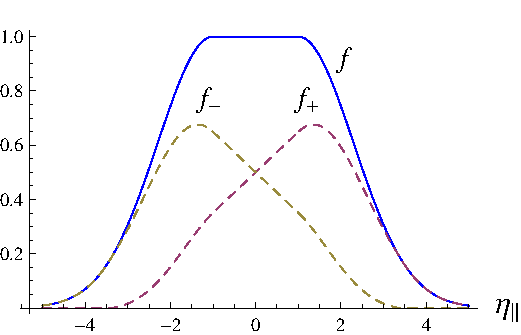
\includegraphics[width=.75\linewidth]{figs/chapter_fbcorr/cartoon_fb.pdf}
\caption{Cartoon showing particle production as a function of $\eta$. $f_+$ and $f_-$ correspond to the forward and backward emission functions respectively.}
\label{fig:fbcorr_cartoon_fb}
\end{figure}

On the other hand, short-range correlations can also be generated dynamically including resonance decay, jet fragmentation, and Bose-Einstein correlations. These correlations are typically localized over a smaller range of the $\eta$ and can be sensitive to final state effects. We will discuss the influences of short-range correlations in the ATLAS data analysis (see Section~\ref{sec:fb_atlas_data}).



\subsubsection{Previous studies and their limitations}

Most previous studies of the longitudinal multiplicity correlation are limited to two rapidity windows symmetric around the center-of-mass of the collision, commonly known as the forward-backward (FB) correlations~\cite{Bialas:2010zb}. The correlation strength is defined by the dependence of the average charged particle multiplicity in the backward hemisphere, $\lr{N_b}$, on the event multiplicity in the forward hemisphere, $N_f$, such that $\lr{N_b} = a + b N_f$, where $a$ is a constant and $b$ measures the correlation strength:
\begin{equation}
b = \frac{\lr{N_f N_b} - \lr{N_f}\lr{N_b}}{\lr{N_f^2} - \lr{N_f}^2} = \frac{D_{bf}^2}{D_{ff}^2}
\end{equation}
where $D_{bf}^2$ (covariance) and $D_{ff}^2$ (variance) are the backward-forward and forward-forward dispersions, respectively~\cite{Abelev:2009ag}. Since $N_f$ and $N_b$ are taken from two symmetric $\eta$ windows at $(\eta, -\eta)$, $\Delta\eta$ is used to quantify the separation of two windows. Correlation strength and similar observables have been measured experimentally in $e^+ e^-$~\cite{Braunschweig:1989bp}, $pp$~\cite{Uhlig:1977dc, ATLAS:2012as, Adam:2015mya}, $p\bar{p}$~\cite{Ansorge:1988fg, Alexopoulos:1995ft} and $A+A$~\cite{Abelev:2009ag} collisions where significant FB asymmetric component has been identified.

Figure~\ref{fig:fbcorr_star_fb} shows the FB correlation strength $b$ as a function of $\Delta\eta$ for $pp$ and centrality selected Au+Au collisions. It is observed that the magnitude of the FB correlation strength decreases with the decrease in centrality. The FB correlation strength evolves from a nearly flat function for $0-10\%$ to a sharply decreasing function with $\Delta\eta$ for the $40-50\%$ and $50-80\%$ centrality bins. Figure~\ref{fig:fbcorr_star_fb} also shows that the dependence of the FB correlation strength with $\Delta\eta$ is quite different in central Au+Au compared to $pp$ collisions.

\begin{figure}[H]
\centering
\includegraphics[width=.7\linewidth]{figs/chapter_fbcorr/star_fb.pdf}
\caption{(b) FB correlation strength for $10-20$, $20-30$, $30-40$, $40-50$ and $50-80\%$ Au+Au and (c) for $pp$ collisions as function of $\Delta\eta$ at $\sqrt{s_\text{NN}}=200$ GeV. The error bars represent the systematic point-to-point error. The boxes show the correlated systematic errors. This figure is taken from Ref.~\cite{Abelev:2009ag}.}
\label{fig:fbcorr_star_fb}
\end{figure}

However, there are few puzzles associated with these measurements, e.g., why correlation strength is stronger in central collisions, where the wounded nucleon fluctuations are smaller? How the short-range correlations affect the results? These questions reflect the limitations of previous correlation strength measurements:
\begin{itemize}
\item Correlation strength $b$ only measures multiplicity correlations in symmetric $\eta$ windows, hence lack of important information such as correlation between mid-rapidity and forward-rapidity;
\item Correlation strength $b$ is diluted by the variance in the denominator. This might explain the observed centrality dependence of the signal: peripheral events have larger tracking efficiency and statistical fluctuation, which leads to smaller $b$;
\item Short-range correlations usually extend to $\Delta\eta \sim 1$, and observed $\Delta\eta$-dependence for $\Delta\eta < 1$ might be due to the residual short-range correlations.
\end{itemize}

Recently, to address all of the limitations above, the forward-backward multiplicity correlation studies are extended by decomposing $N(\eta)$ into Chebyshev polynomials~\cite{Bzdak:2012tp} or into principle components~\cite{Bhalerao:2014mua}, with each mode representing the different components of the measured FB correlation. In our studies, we further extend the existing method by proposing a single-particle method that obtains these shape components directly from each event, as well as a two-particle correlation method that gives the ensemble RMS average of these shape components. We apply the method to HIJING and AMPT models and successfully extract the different shape components of the multiplicity fluctuation. The first component is found to be found to be directly related to the long-range asymmetry of the fireball, while the higher-order components are more related to the short-range correlations. The extracted components are also found to be dampened by the final-state interactions. To suppress the short-range correlations, the newly proposed correlators are measured with same and opposite changed particles separately, and this suppression technique is applied to the ATLAS data, as well as the QCD-inspired models such as PYTHIA~\cite{Sjostrand:2007gs} and EPOS~\cite{Pierog:2013ria}, to reveal the longitudinal multiplicity fluctuations in $pp$, $p$+Pb and Pb+Pb collision systems.



\subsection{Methodology}

\subsubsection{Observables}

\paragraph{Single-particle method}

Following previous notations, in a single event, the number of charged particles (multiplicity) in a given $\eta$ window is denoted as $N(\eta)$. To get rid of the average multiplicity, we define a normalized quantity $\rho(\eta)$:
\begin{equation}
\rho(\eta) \equiv \frac{N(\eta)}{\lr{N(\eta)}},
\end{equation}
where $\lr{N(\eta)}$ is the average distribution for a given event-multiplicity class. Legendre polynomials $P_n(x)$:
\begin{equation}
\begin{split}
P_0(x) &= 1 \\
P_1(x) &= x \\
P_2(x) &= \frac{1}{2}(3x^2 - 1)
\end{split}
\end{equation}
are used to quantify the shape of longitudinal multiplicity fluctuation. The particle density $\rho(\eta)$ in the interval $[-Y, Y]$ is then written in terms of Legendre polynomials:
\begin{equation}
\begin{split}
\rho(\eta) &\propto 1 + \sum a_n T_n(\eta) \\
T_n(\eta) &\equiv \sqrt{\frac{2n+1}{3}} Y P_n(\frac{\eta}{Y})
\end{split}
\end{equation}
where $a_n$ is the coefficient to be measured and the scaling factor $\sqrt{\frac{2n+1}{3}}$ is chosen such that $T_1(\eta)=\eta$.



\paragraph{Two-particle correlation method}

Single particle density $\rho(\eta)$ cannot be measured as an average over many similar events, due to $\lr{\rho(\eta)} = 1$. Thus the two-particle correlation function in $\eta$ is defined as:
\begin{equation}
C(\eta_1, \eta_2) \equiv \frac{\lr{N(\eta_1)N(\eta_2)}}{\lr{N(\eta_1)}\lr{N(\eta_2)}} = \lr{\rho(\eta_1)\rho(\eta_2)},
\end{equation}
where again the $N(\eta)$ is the multiplicity density distribution in a single event and $\lr{N(\eta)}$ is the average distribution for a given event-multiplicity class. The correlation function is directly related to a single-particle quantity $\rho(\eta)$, which characterizes the fluctuation of multiplicity in a single event relative to the average shape of the event class.

Compared with the correlation strength $b$, $C(\eta_1, \eta_2)$ has two advantages:
\begin{itemize}
\item $\eta_1$ and $\eta_2$ are not necessarily symmetric about zero, which makes $C(\eta_1, \eta_2)$ measures all possible correlated pairs in the full $\eta$ ranges $[-Y, Y]$;
\item The denominator of $C(\eta_1, \eta_2)$ is no longer a variance, thus tracking efficiency and statistical fluctuations have no influences on this new observable. 
\end{itemize}

In the single particle method, by construction, $\lr{a_n} = 0$. In the two-particle correlation method, we are going to measure $\lr{a_n a_m}$. Plug the $\rho(\eta)$ into the definition of $C(\eta_1, \eta_2)$ and we have:
\begin{equation}
C(\eta_1, \eta_2) = 1 + \sum \lr{a_n a_m} T_n(\eta_1) T_m(\eta_2)
\end{equation}
where $\lr{a_n a_m} \neq 0$, and this is one of the reasons why two particle correlation method is introduced. The shapes of the first two bases $T_n(\eta_1)T_m(\eta_2)$ are shown in Figure~\ref{fig:fbcorr_Legendre_base_2D}.

\begin{figure}[H]
\centering
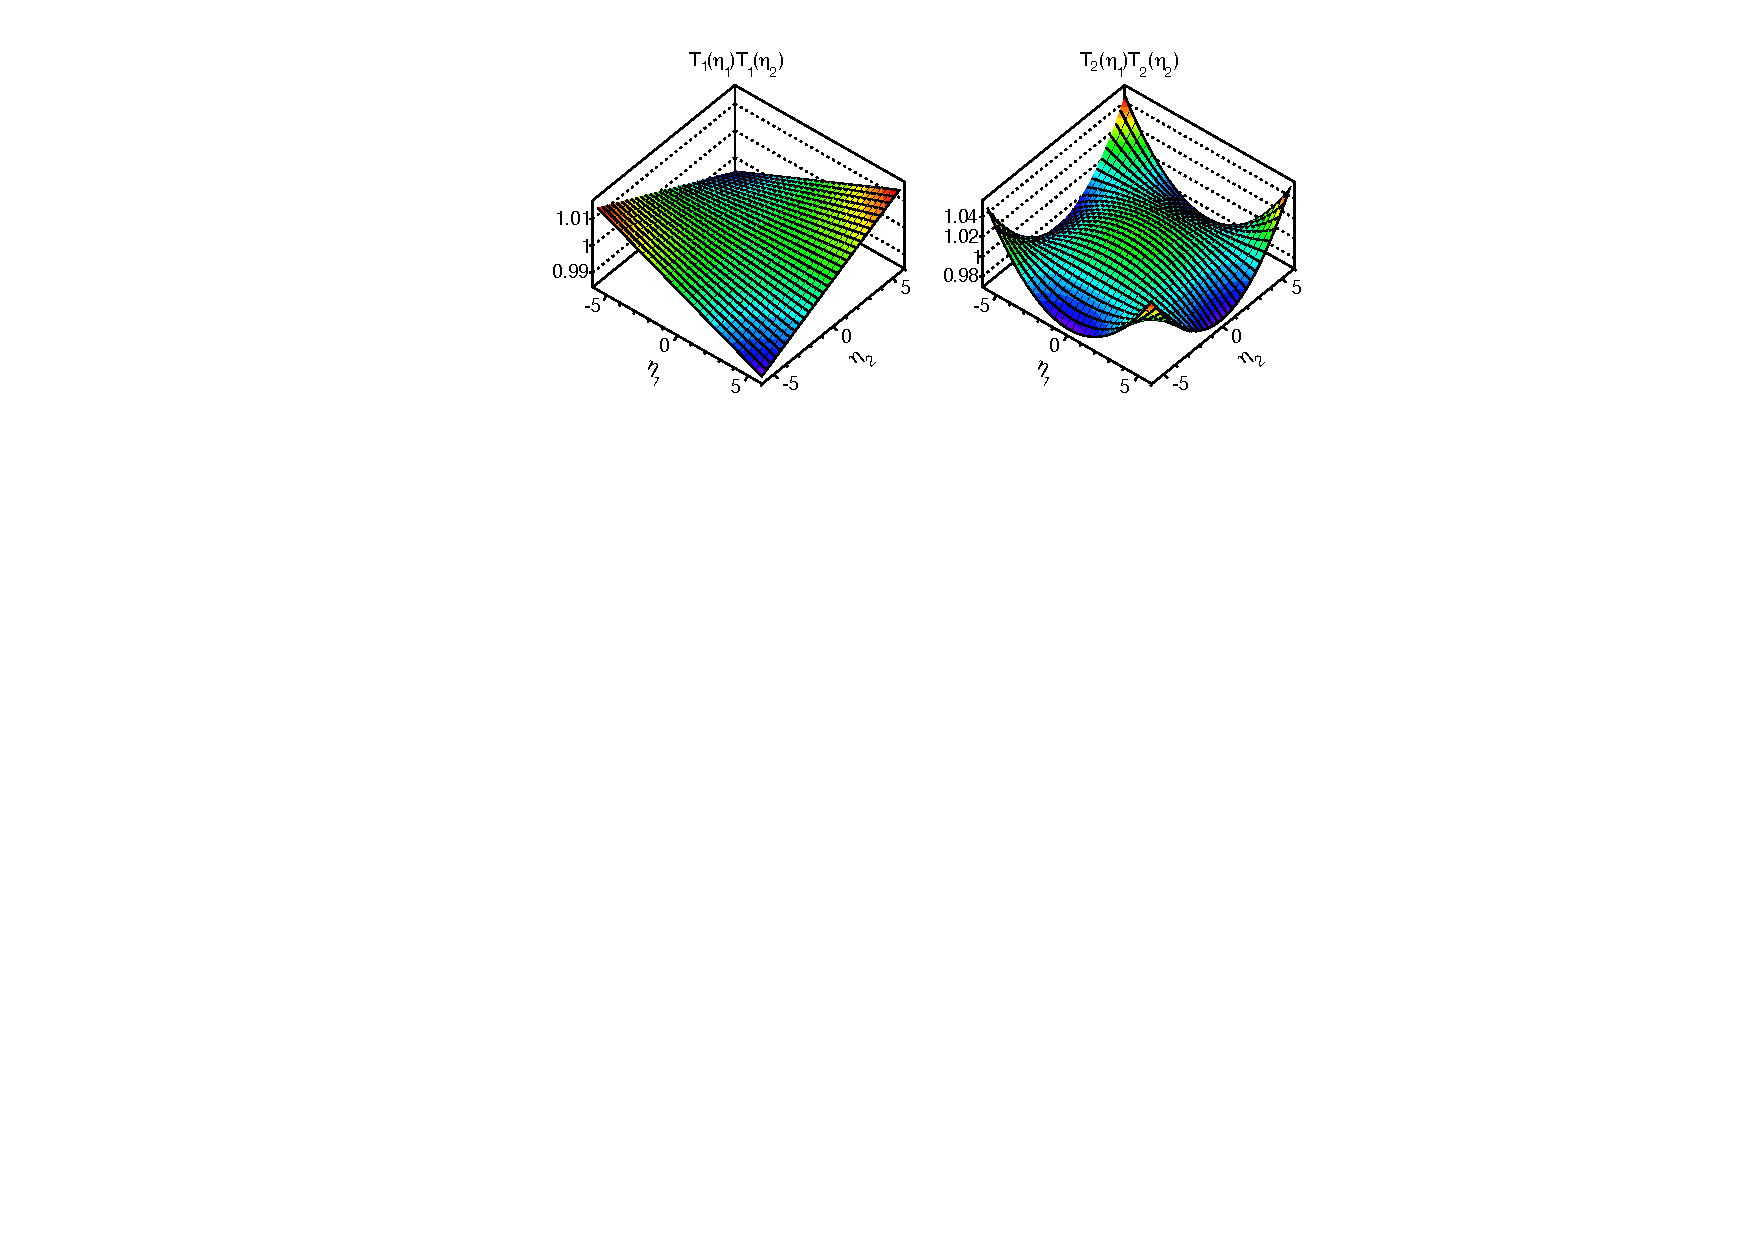
\includegraphics[width=.95\linewidth]{figs/chapter_fbcorr/Legendre_base_2D.pdf}
\caption{The shape of the first two bases associated with $\lr{a_n a_m}$ in the two-particle correlation function. They are plotted assuming $\lr{a_n a_m}=0.01$.}
\label{fig:fbcorr_Legendre_base_2D}
\end{figure}

Using the orthogonal relations of the Legendre polynomials:
\begin{equation}
\begin{split}
\int_{-Y}^Y T_n(\eta) d\eta &= 0 \\
\int_{-Y}^Y T_n(\eta) T_m(\eta) d\eta &= \frac{2Y^2}{3}\delta_{nm}
\end{split}
\end{equation}
where factor $\frac{2Y^2}{3}$ remains because of the scaling factor $\sqrt{\frac{2n+1}{3}}$ in the definition of $T_n(\eta)$, one could calculate the two-particle Legendre coefficients directly:
\begin{equation}
\lr{a_n a_m} = (\frac{3}{2Y^3})^2 \int_{-Y}^Y C(\eta_1, \eta_2) T_n(\eta_1) T_m(\eta_2) d\eta_1 d\eta_2
\end{equation}
One of the reasons we prefer Legendre polynomials to Chebyshev polynomials~\cite{Bzdak:2012tp} is that in the orthogonal relation of Legendre polynomials, there is no additional weight as a function of $\eta$. The two-particle correlation method measures, in effect, the RMS values of the EbyE $a_n$, $\sqrt{\lr{a_n^2}}$, or the cross correlation between $a_n$ and $a_m$, $\lr{a_n a_m}$. The correlation functions satisfy the symmetric condition $C(\eta_1, \eta_2) = C(\eta_2, \eta_1)$.

Among all the terms of $\lr{a_n a_m}$, terms such as $\lr{a_0 a_n}$ involve the correlation between shape fluctuation $a_n$ and the overall multiplicity fluctuation $a_0$. Provided all deviations from one are small, the terms involving $\lr{a_0 a_n}$ can be removed. We define normalized two-particle correlation $C_N(\eta_1, \eta_2)$:
\begin{equation}
\begin{split}
C_N(\eta_1, \eta_2) &= \frac{C(\eta_1, \eta_2)}{C_p(\eta_1) C_p(\eta_2)} \\
C_p(\eta_1) &= \frac{\int_{-Y}^Y C(\eta_1, \eta_2) d\eta_2}{2Y} \\
C_p(\eta_2) &= \frac{\int_{-Y}^Y C(\eta_1, \eta_2) d\eta_1}{2Y}
\end{split}
\end{equation}
where the quantities $C_p(\eta_1)$ and $C_p(\eta_2)$ are referred to as the single-particle modes. The $\lr{a_0 a_0}$ term can be removed by renormalizing average value in the $\eta_1$, $\eta_2$ phase space to be one.



\subsubsection{Removal of short-range correlation}

\paragraph{Outline}

The aim of our studies is to measure and parametrize the long-range correlation (LRC), which requires the separation and subtraction of the short-range correlation (SRC). The separation of SRC and LRC is quite involved and so is briefly summarized here, with details left to the sections below.

The core of the separation method is to exploit the difference between the correlations for opposite-charge and same-charge pairs, $C^{+-}(\eta_1, \eta_2)$ and $C^{\pm\pm}(\eta_1, \eta_2)$, respectively. The SRC component centered around $\eta_- \equiv \eta_1 - \eta_2 \sim 0$ is found to be much stronger for opposite-charge pairs, primarily due to local charge conservation, while the LRC and single-particle modes are expected to be independent of the charge combination. With this assumption, the ratio $R(\eta_1, \eta_2)$ can be approximated by:
\begin{equation}
\begin{split}
R(\eta_1, \eta_2) &= \frac{C^{+-}(\eta_1, \eta_2)}{C^{\pm\pm}(\eta_1, \eta_2)} \\
&= \frac{1 + C_\text{LRC}^{+-}(\eta_1, \eta_2) + \dSo(\eta_1, \eta_2)}{1 + C_\text{LRC}^{\pm\pm}(\eta_1, \eta_2) + \dSs(\eta_1, \eta_2)} \\
&\approx 1 + \dSo(\eta_1, \eta_2) - \dSs(\eta_1, \eta_2)
\end{split}
\end{equation}
where $C_\text{LRC}(\eta_1, \eta_2)$ and $\delta_\text{SRC}(\eta_1, \eta_2)$ represent the correlations for LRC and SRC separately. The results can be approximated because both LRC and SRC are significantly smaller than one.

Our studies further assume that the dependence of $\delta_\text{SRC}$ on $\eta_-$ and $\eta_+ \equiv \eta_1 + \eta_2$ factorizes and that the dependence on $\eta_+$ is independent of the charge combinations
\begin{equation}
\begin{split}
\dSo(\eta_+, \eta_-) &= f(\eta_+)g^{+-}(\eta_-) \\
\dSs(\eta_+, \eta_-) &= f(\eta_+) g^{\pm\pm}(\eta_-)
\end{split}
\end{equation}
where $g^{+-}(\eta_-)$ and $g^{\pm\pm}(\eta_-)$ are allowed to differ in both shape and magnitude. The validity of these various assumptions is confirmed in the data from the extracted $\delta_{SRC}^{+-}(\eta_+, \eta_-)$ and $\delta_{SRC}^{\pm\pm}(\eta_+, \eta_-)$ after applying the separation procedure. With these assumptions, $f(\eta_+)$ can be determined from $R$ by suitable integration over $\eta_-$, as described in Section~\ref{sec:probing_the_src_via_the_same_charge_and_opposite_charge_correlations}.

To complete the determination of $\dSs$, the quantity $g^{\pm\pm}$ is determined and parameterized from suitable projections of $C_N^{\pm\pm}(\eta_+, \eta_-)$ in the $\eta_-$ direction, as described in Section~\ref{sec:separation_of_the_src_and_the_lrc}. The use of $C_N^{\pm\pm}$ rather than $C^{\pm\pm}$ is because the former does not contain the single-particle modes. The procedure to obtain a correlation function with the SRC subtracted is also described in Section~\ref{sec:separation_of_the_src_and_the_lrc}. With $\dSs$ determined, $\dSo$ can be obtained directly. The $\dSs$ and $\dSo$ are then averaged to obtain the SRC for all charge combinations, $\delta_\text{SRC}$.

This SRC estimation technique is mainly applied to the ATLAS data, and briefly tested on PYTHIA and EPOS MC samples. For demonstration purpose, Pb+Pb and $p$+Pb collision systems are discussed in the section.



\paragraph{Probing the SRC via the same-charge and opposite-charge correlations}
\label{sec:probing_the_src_via_the_same_charge_and_opposite_charge_correlations}

Figure~\ref{fig:fbcorr_ATLAS_SRCremoval_PbPb} shows separately the correlation functions for same-charge pairs and opposite-charge pairs from Pb+Pb collisions with $200 \le \Nchrec < 220$. The ratio of the two, $R(\eta_1, \eta_2)$, is shown in the top right panel. The correlation functions show a narrow ridge-like shape along $\eta_1 \approx \eta_2$ or $\eta_- \approx 0$, and a falloff towards the corners at $\eta_1 = -\eta_2 \approx \pm 2.4$. The magnitude of the ridge for the opposite-charge pairs is stronger than that for the same-charge pairs, which is characteristic of the influence from SRC from jet fragmentation or resonance decays. In regions away from the SRC, i.e., large values of $|\eta_-|$, the ratio approaches unity, suggesting that the magnitude of the LRC is independent of the charge combinations. To quantify the shape of the SRC in the ratio along $\eta_+$, $R$ is expressed in terms of $\eta_+$ and $\eta_-$, $R(\eta_+, \eta_-)$, and the following quantity is calculated:
\begin{equation}
f(\eta_+) = \frac{\frac{1}{0.8} \int_{-0.4}^{0.4} R(\eta_+, \eta_-)d\eta_- - 1}{\frac{1}{0.8} \int_{-0.4}^{0.4} R(0, \eta_-)d\eta_- - 1}
\end{equation}
As shown in Figure~\ref{fig:fbcorr_ATLAS_SRCremoval_PbPb}, the quantity $f(\eta_+)$ is nearly constant in Pb+Pb collisions, implying that the SRC is consistent with being independent of $\eta_+$. To quantify the shape of the SRC along the $\eta_-$ direction, $R(\eta_+, \eta_-)$ is fitted to a Gaussian function in slices of $\eta_+$. The width, as shown in the bottom middle panel of Figure~\ref{fig:fbcorr_ATLAS_SRCremoval_PbPb}, is constant, which may suggest that the shape of the SRC in $\eta_-$ is the same for different $\eta_+$ slices.

\begin{figure}[H]
\centering
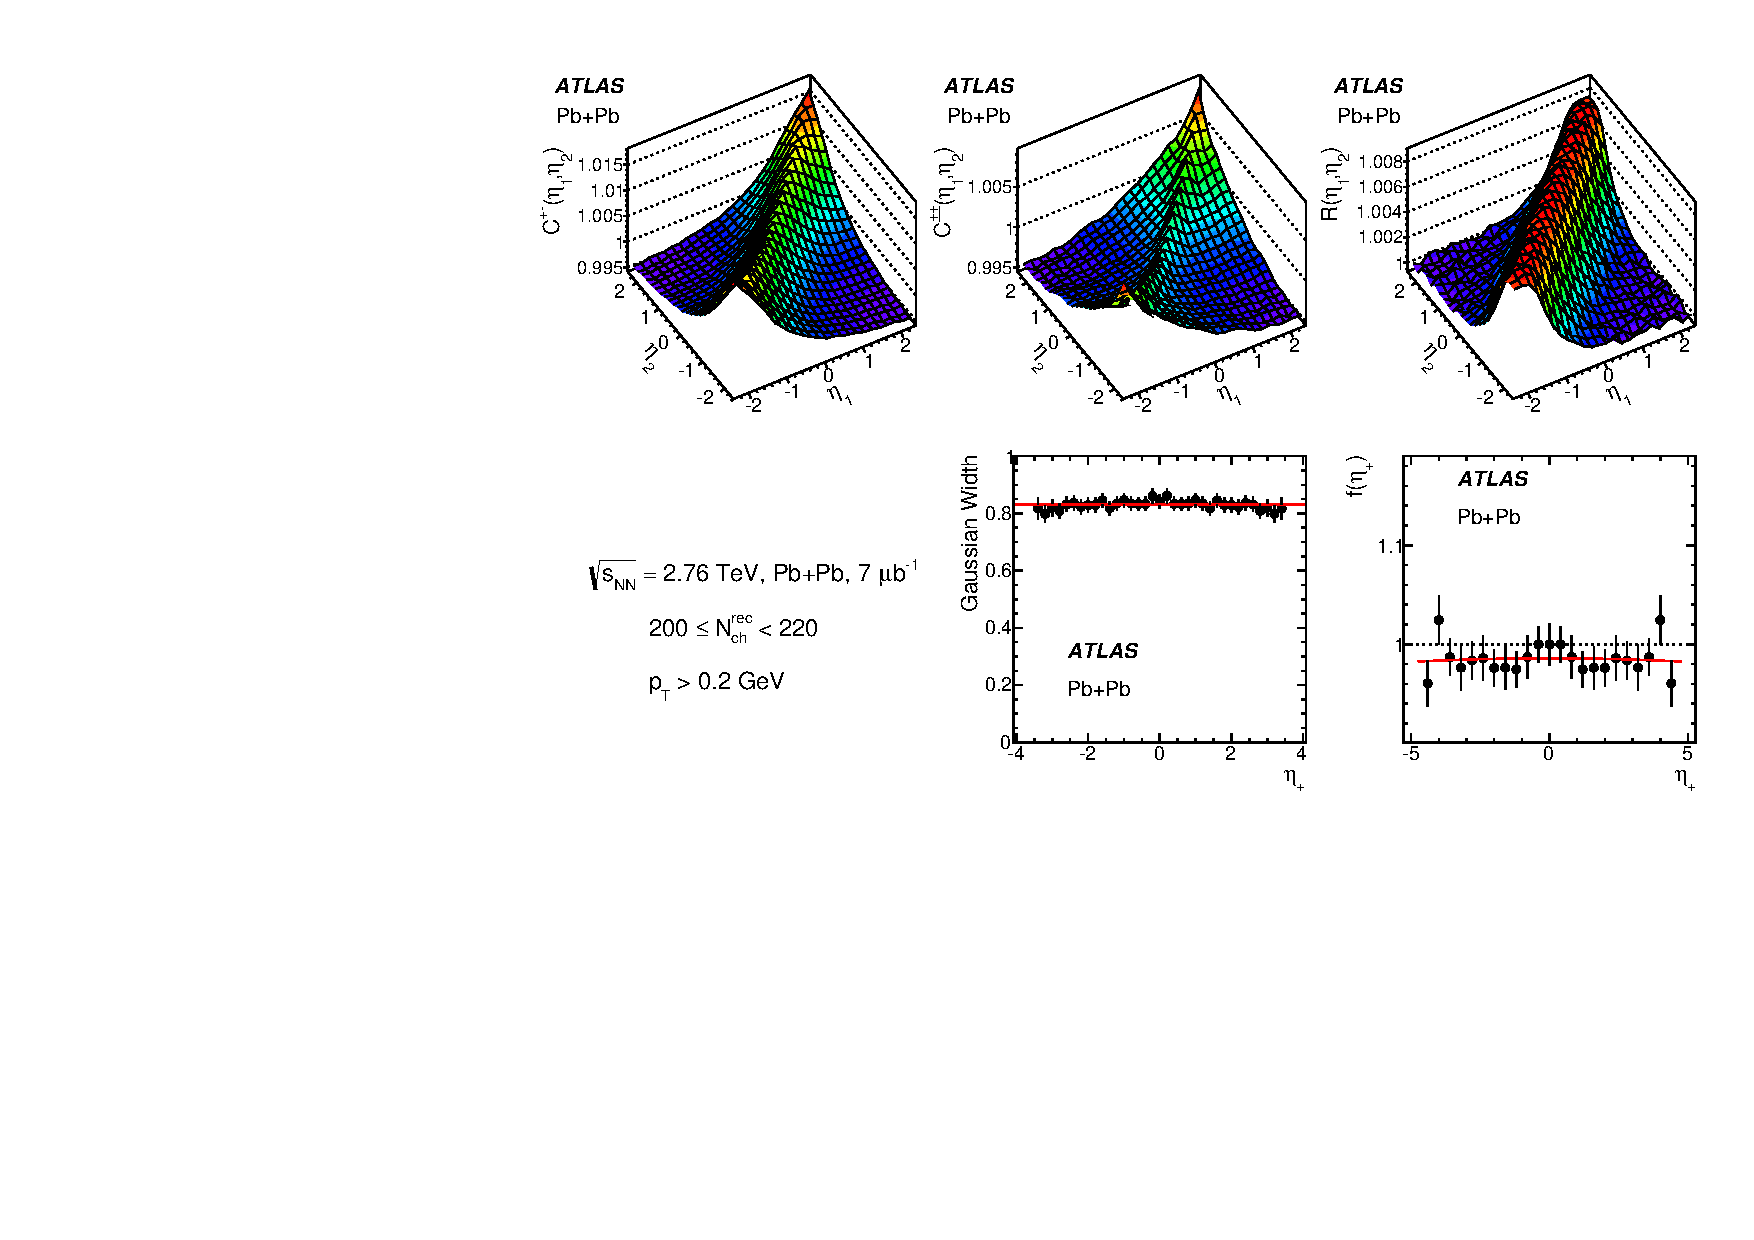
\includegraphics[width=.95\linewidth]{figs/chapter_fbcorr/ATLAS_SRCremoval_PbPb.pdf}
\caption{The correlation functions for opposite-charge pairs $C^{+-}(\eta_1, \eta_2)$ (top left), same-charge pairs $C^{\pm\pm}(\eta_1, \eta_2)$ (top middle) and the ratio $R(\eta_1, \eta_2)$ (top right) for Pb+Pb collisions with $200 \le \Nchrec < 220$. The width and magnitude of the short-range Gaussian peak of the ratio are shown in the lower middle and right panels. The error bars represent the statistical uncertainties, and the solid lines indicate a quadratic fit.}
\label{fig:fbcorr_ATLAS_SRCremoval_PbPb}
\end{figure}

Figure~\ref{fig:fbcorr_ATLAS_SRCremoval_pPb} shows the correlation function in $p$+Pb collisions with multiplicity similar to the Pb+Pb data in Figure~\ref{fig:fbcorr_ATLAS_SRCremoval_PbPb}. The correlation function shows a significant asymmetry between the proton-going side (positive $\eta_+$) and lead-going side (negative $\eta_+$). However, much of this asymmetry appears to be confined to a small $|\eta_-|$ region where the SRC dominates. The magnitude of the SRC, estimated by $f(\eta_+)$ shown in the bottom-right panel, increases by about $50\%$ from the lead-going side (negative $\eta_+$) to the proton-going side (positive $\eta_+$), but the width of the SRC in $\eta_-$ is independent of $\eta_+$ as shown in the bottom-middle panel. In contrast, the LRC has no dependence on the charge combinations, since the value of $R$ approaches unity at large $|\eta_-|$.

\begin{figure}[H]
\centering
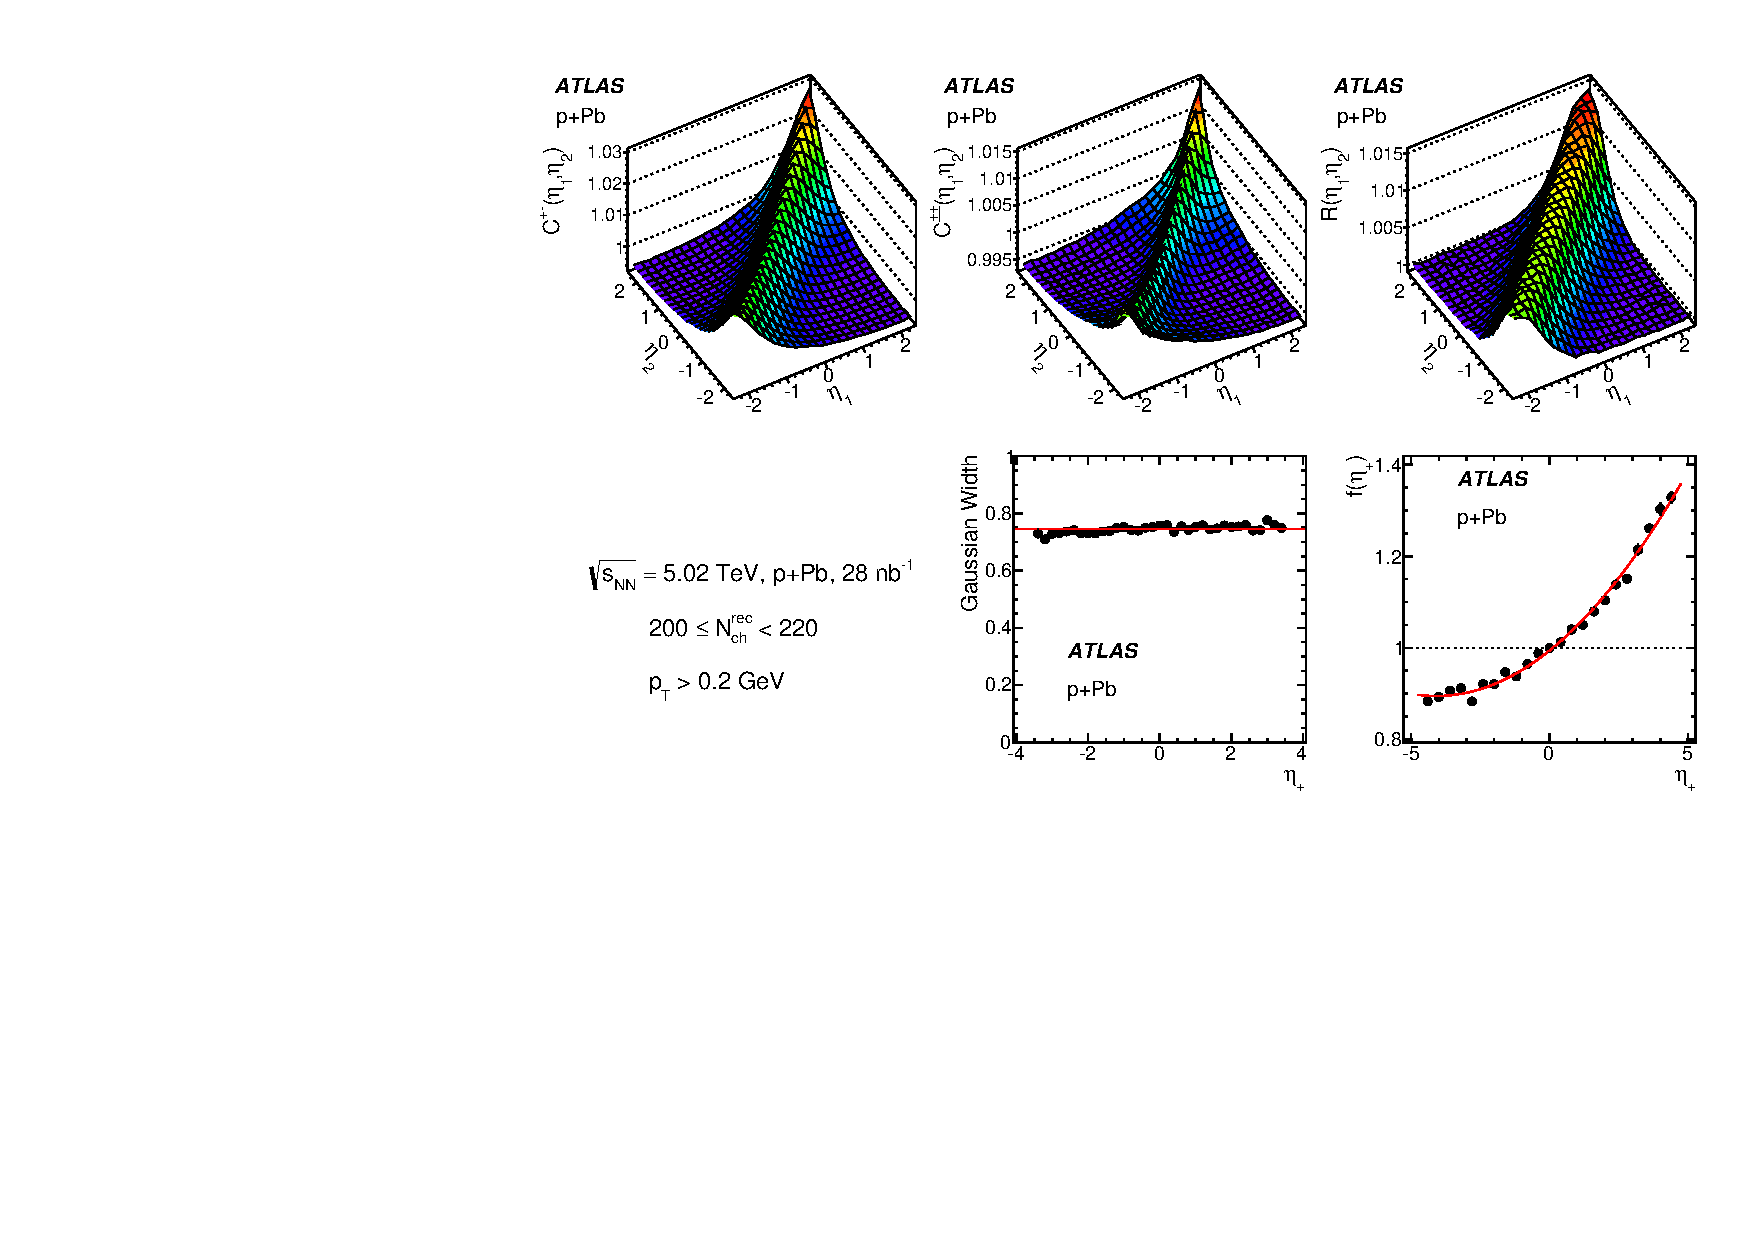
\includegraphics[width=.95\linewidth]{figs/chapter_fbcorr/ATLAS_SRCremoval_pPb.pdf}
\caption{The correlation functions for opposite-charge pairs $C^{+-}(\eta_1, \eta_2)$ (top left), same-charge pairs $C^{\pm\pm}(\eta_1, \eta_2)$ (top middle) and the ratio $R(\eta_1, \eta_2)$ (top right) for $p$+Pb collisions with $200 \le \Nchrec < 220$. The width and magnitude of the short-range Gaussian peak of the ratio are shown in the lower middle and right panels. The error bars represent the statistical uncertainties, and the solid lines indicate a quadratic fit.}
\label{fig:fbcorr_ATLAS_SRCremoval_pPb}
\end{figure}

Left panel of Figure~\ref{fig:fbcorr_ATLAS_SRCremoval_sysComp} shows the width in $\eta_-$ of the short-range component as a function of $\Nch$ in the three collision systems. The width is obtained as the Gaussian width of $R(\eta_+, \eta_-)$ in the $\eta_-$ direction, and then averaged over $\eta_+$ as the width is observed to be independent of $\eta_+$, as shown in Figure~\ref{fig:fbcorr_ATLAS_SRCremoval_PbPb} and~\ref{fig:fbcorr_ATLAS_SRCremoval_pPb}. This width reflects the extent of the short-range correlation in $\eta$, and it is observed to decrease with increasing $\Nch$ in all collision systems. At the same $\Nch$ value, the width is smallest in $pp$ collisions and largest in Pb+Pb collisions. In the right panel of Figure~\ref{fig:fbcorr_ATLAS_SRCremoval_sysComp}, the width of the short-range component from $pp$ data is compared with PYTHIA 8 based on the A2 tune~\cite{ATL-PHYS-PUB-2011-014} and EPOS based on the LHC tune~\cite{Pierog:2013ria}. The width of is underestimated by PYTHIA 2 A2 and overestimated by EPOS LHC.

\begin{figure}[H]
\centering
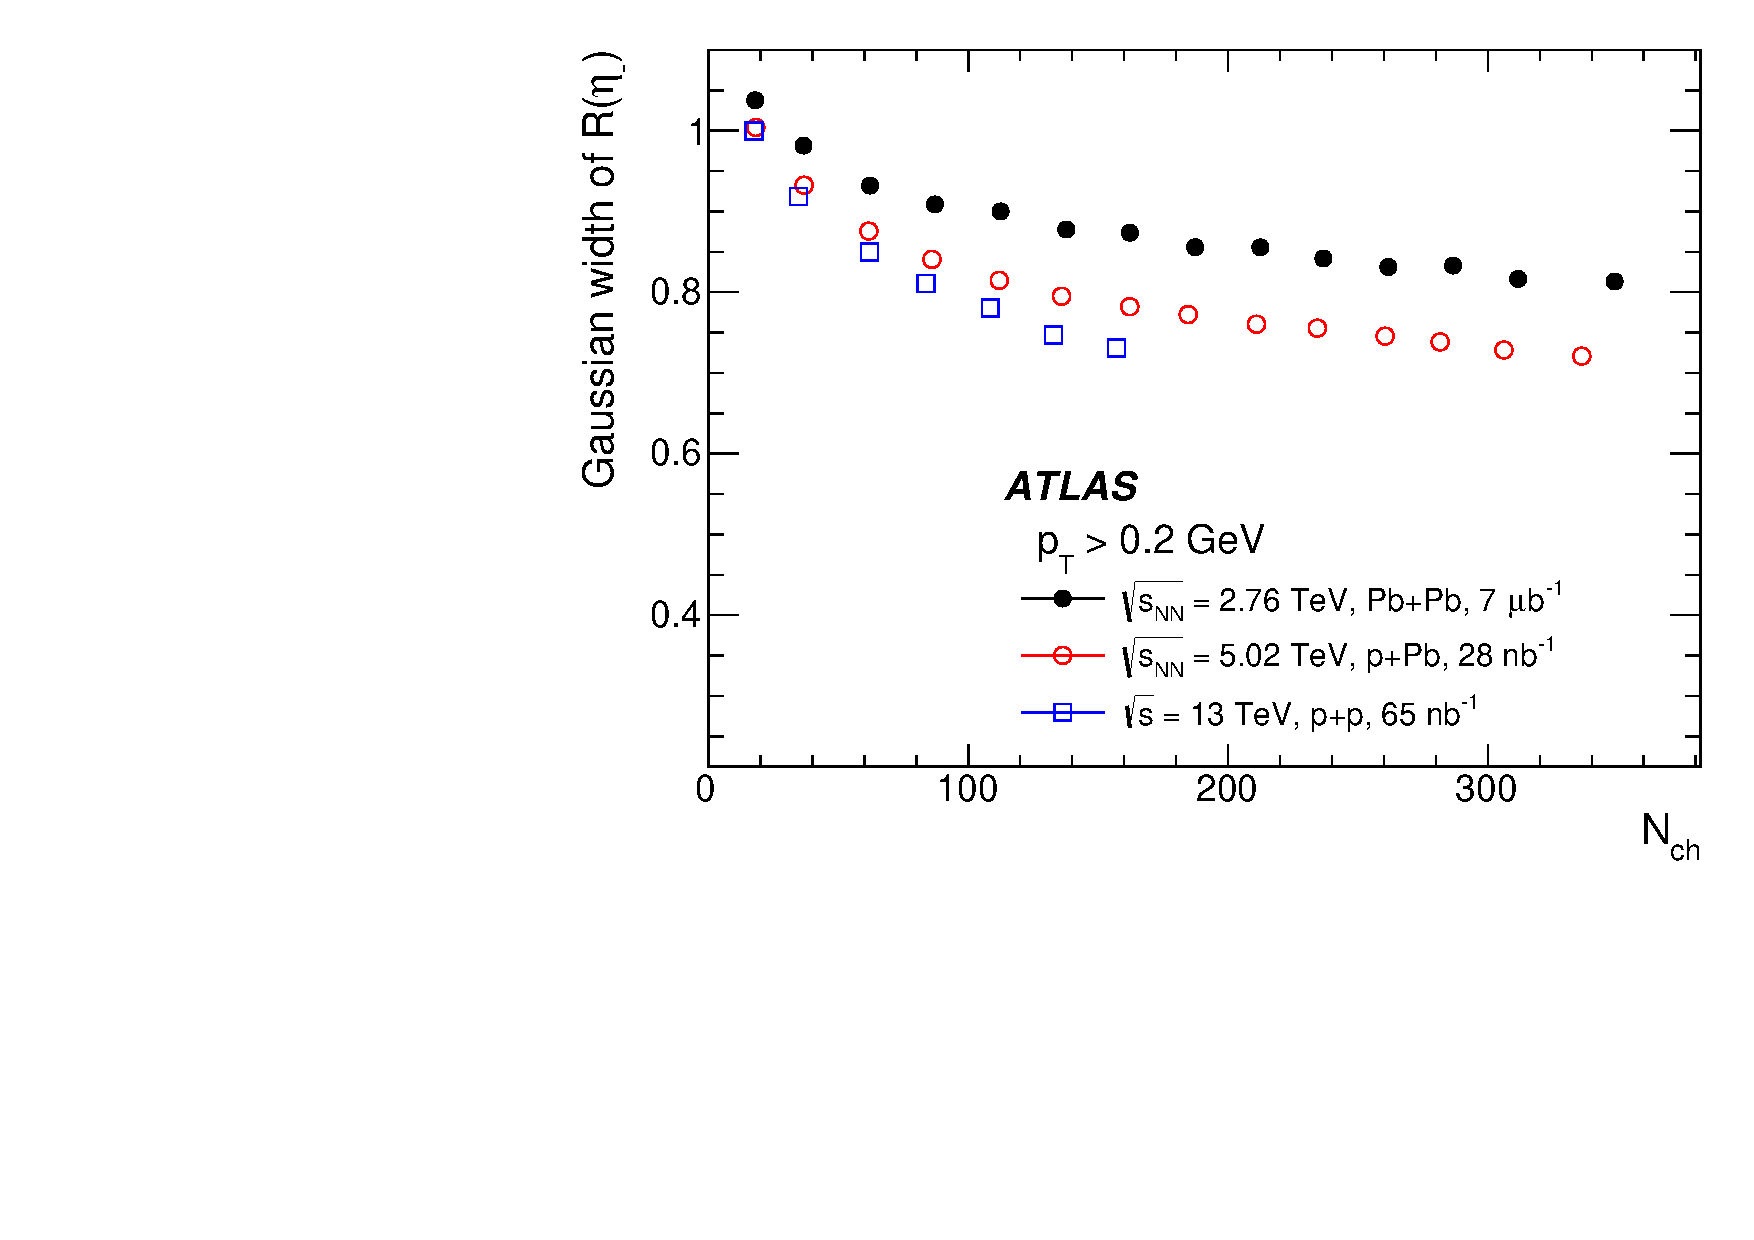
\includegraphics[width=.475\linewidth]{figs/chapter_fbcorr/ATLAS_SRCremoval_sysComp.pdf}
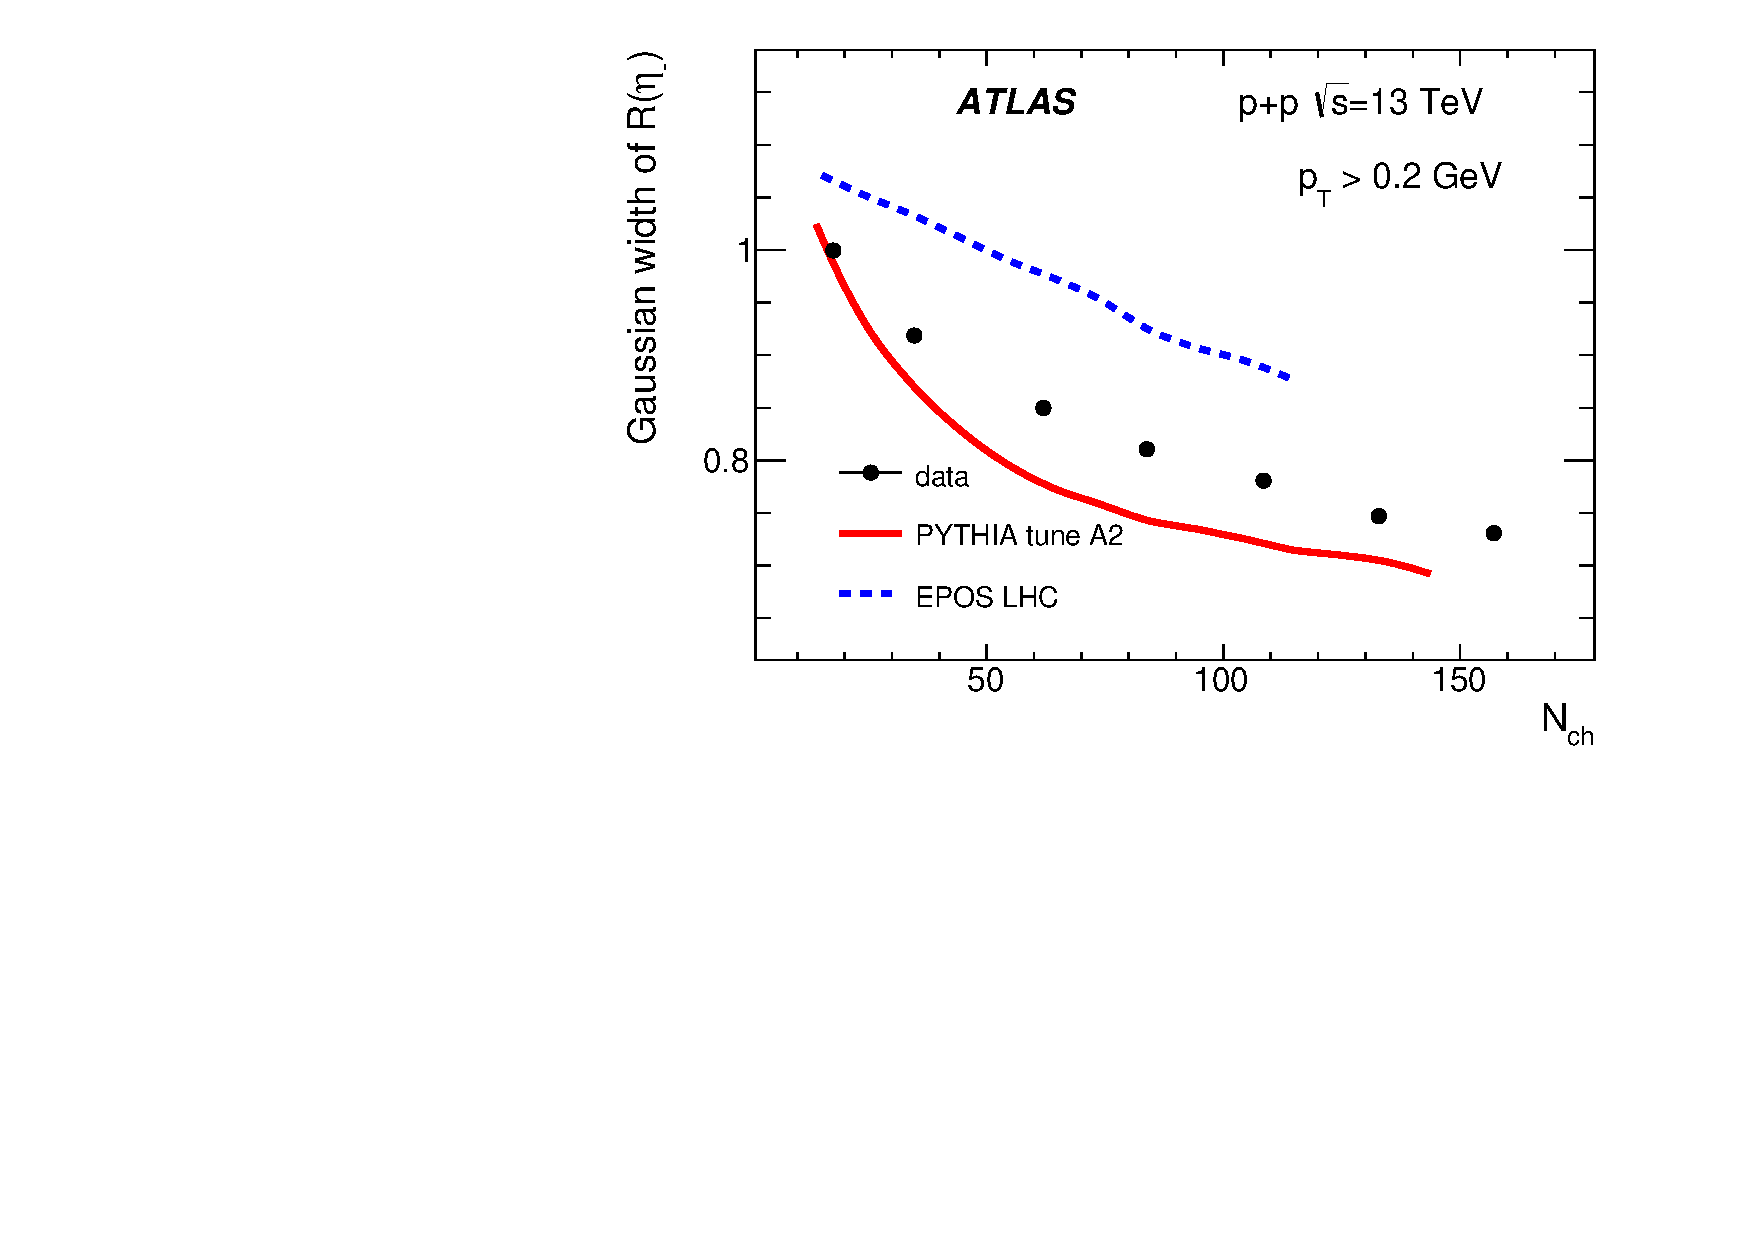
\includegraphics[width=.475\linewidth]{figs/chapter_fbcorr/ATLAS_SRCremoval_modelComp.pdf}
\caption{The width of the short-range component in $R(\eta_+, \eta_-)$ along the $\eta_-$ direction as a function of $\Nch$: in three collision systems (left), compared between data and two models.}
\label{fig:fbcorr_ATLAS_SRCremoval_sysComp}
\end{figure}



\paragraph{Separation of the SRC and the LRC}
\label{sec:separation_of_the_src_and_the_lrc}

As discussed before, the ratio of the correlation function between opposite-charge and same-charge pairs $R(\eta_+, \eta_-)$ is the key to the separation of the SRC and LRC. Following above equations, this ratio can be approximated by:
\begin{equation}
\begin{split}
R(\eta_+, \eta_-) &\approx 1 + f(\eta_+) [g^{+-}(\eta_-) - g^{\pm\pm}(\eta_-)] \\
\dSo &= f(\eta_+) g^{+-}(\eta_-) \\
\dSs &= f(\eta_+) g^{\pm\pm}(\eta_-)
\end{split}
\end{equation}
where $f(\eta_+)$ describes the magnitude along $\eta_+$ and can be calculated from $R(\eta_+, \eta_-)$. The functions $g^{+-}$ and $g^{\pm\pm}$ describe the SRC along the $\eta_-$ direction for the two charge combinations, which differ in both magnitude and shape.

In order to estimate the $g^{\pm\pm}(\eta_-)$ function for same-charge pairs, the $C_N(\eta_+, \eta_-)$ distributions for same-charge pairs are projection into one-dimensional $\eta_-$ distributions over a narrow slice $|\eta_+|<0.4$. The distributions are denoted by $C_N(\eta_-)$. They are shown, after a small iterative correction discussed below, in the second column of Figure~\ref{fig:fbcorr_ATLAS_SRCremoval_fit} for the same-charge pairs in Pb+Pb and $p$+Pb collisions. The SRC appears as a narrow peak on top of a distribution that has an approximately quadratic shape. Therefore, a quadratic fit is applied to the data in the region of $|\eta_-|>1.5$, and the difference between the data and fit in the $|\eta_-|<2$ region is taken as the estimated SRC component or the $g^{\pm\pm}(\eta_-)$ function, which is assumed to be zero for $|\eta_-|>2$. This range ($|\eta_-|>1.5$) is about twice the width of the short-range peak in the $R(\eta_+, \eta_-)$ distribution along the $\eta_-$ distribution. This width is observed to decrease from 1.0 to 0.7 as a function of $\Nchrec$ in the $p$+Pb collisions, and is slightly broader in Pb+Pb collisions and slightly narrower in $pp$ collisions at the same $\Nchrec$. The range of the fit is varied from $|\eta_-|>1.0$ to $|\eta_-|>2.0$ to check the sensitivity of the SRC estimation, and the variation is included in the final systematic uncertainties. Furthermore, this study is also repeated for $C_N(\eta_-)$ obtained in several other $\eta_+$ slices within $|\eta_+|<1.2$, and consistent results are obtained. Once the distribution $g^{\pm\pm}(\eta_-)$ for same-charge pairs is obtained from the fit, it is multiplied by the $f(\eta_+)$ function calculated from $R(\eta_+, \eta_-)$ to obtain the $\delta(\eta_1, \eta_2)$ in the full phase space. Subtracting this distribution from the $C_N(\eta_1, \eta_2)$ distribution, one obtains the initial estimate of the correlation function containing mostly the LRC component.

\begin{figure}[H]
\centering
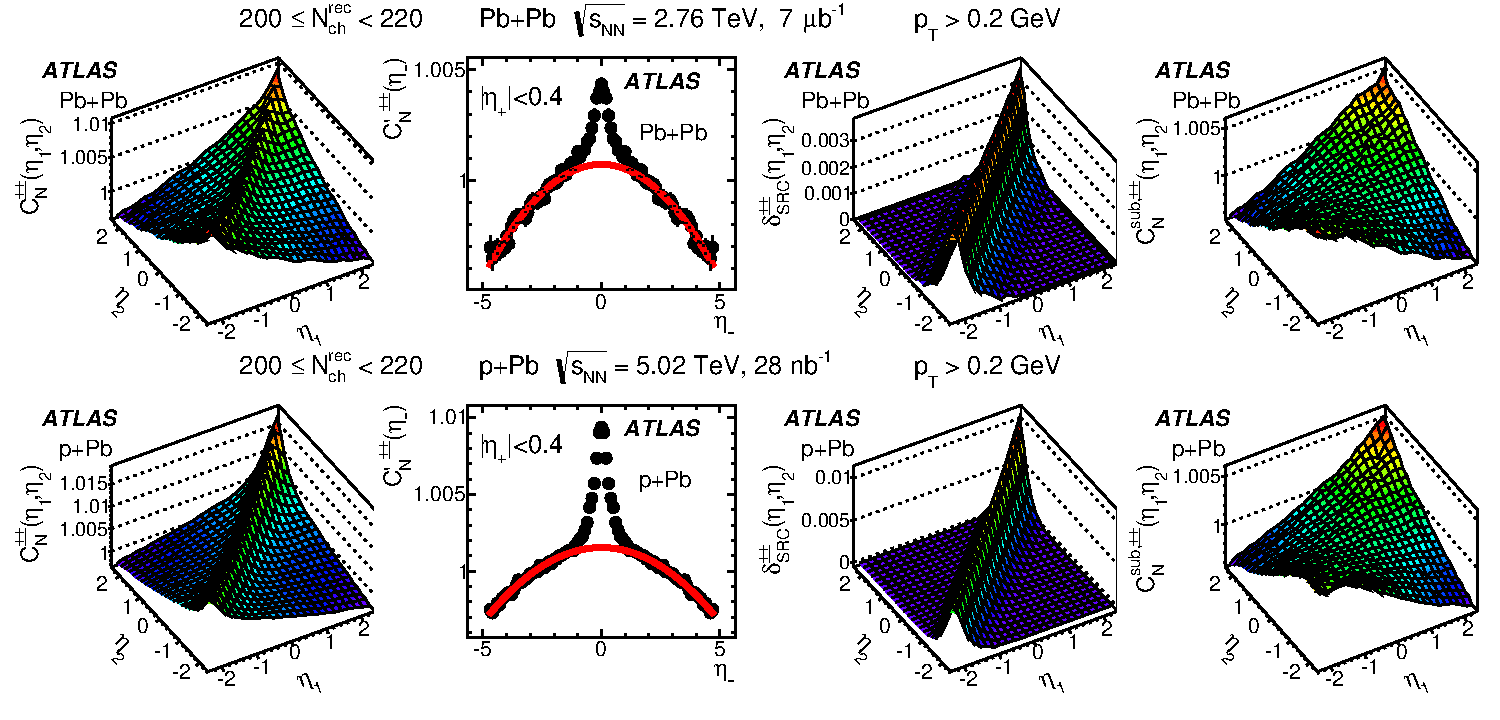
\includegraphics[width=.95\linewidth]{figs/chapter_fbcorr/ATLAS_SRCremoval_fit.pdf}
\caption{The separation of correlation functions for same-charge pairs (first column) into the SRC (third column) and the LRC (last column) for Pb+Pb (top row) and $p$+Pb (bottom row) collisions with $200 \le \Nchrec < 220$. The second column shows the result of the quadratic fit over the $|\eta_-|>1.5$ range of the one-dimensional correlation function projected over the $|\eta_+|<0.4$ slice, which is used to estimate the SRC component. The error bars represent the statistical uncertainties.}
\label{fig:fbcorr_ATLAS_SRCremoval_fit}
\end{figure}



\paragraph{Iterative correction for single-particle mode}

The LRC obtained via this procedure is still affected by a small bias from the SRC via the normalization procedure of $C_N(\eta_1, \eta_2)$. This bias appears because the $\delta_\text{SRC}(\eta_1, \eta_2)$ contribution is removed from the numerator but is still included in the denominator via $C_p(\eta)$. This contribution is not uniform in $\eta$: If the first particle is near mid-rapidity $\eta_1 \approx 0$ then all pairs in $\delta_\text{SRC}(\eta_1, \eta_2)$ contribute to $C_p(\eta_1)$, whereas if the first particle is near the edge of the acceptance $\eta_1 \approx \pm Y$ then only half of the pairs in $\delta_\text{SRC}(\eta_1, \eta_2)$ contribute to $C_p(\eta_1)$. The acceptance bias in $C_p$ is removed via a simple iterative procedure: First, the $\delta_\text{SRC}$ contribution determined from the above procedure is used to eliminate the SRC contribution to the single-particle mode:
\begin{equation}
\begin{split}
C_p^\text{sub}(\eta_1) &= \frac{\int_{-Y}^Y [C(\eta_1, \eta_2) - \delta_\text{SRC}(\eta_1, \eta_2)] d\eta_2}{2Y} \\
C_p^\text{sub}(\eta_2) &= \frac{\int_{-Y}^Y [C(\eta_1, \eta_2) - \delta_\text{SRC}(\eta_1, \eta_2)] d\eta_1}{2Y}.
\end{split}
\end{equation}
The $C_p^\text{sub}(\eta_1)$ and $C_p^\text{sub}(\eta_2)$ are then used to redefine the $C_N$ function:
\begin{equation}
C_N^{'}(\eta_1, \eta_2) = \frac{C(\eta_1, \eta_2)}{C_p^\text{sub}(\eta_1) C_p^\text{sub}(\eta_2)}.
\end{equation}
This distribution, which is very close to the distribution before correction, is shown in the second column of Figure~\ref{fig:fbcorr_ATLAS_SRCremoval_fit} for projection over a narrow slice $|\eta_+|<0.4$. The estimation of $\delta_\text{SRC}(\eta_1, \eta_2)$ is repeated using the previously described procedure for the $C_N^{'}(\eta_1, \eta_2)$, and the extracted distribution is shown in the third column of Figure~\ref{fig:fbcorr_ATLAS_SRCremoval_fit}. Subtracting this distribution from $C_N^{'}(\eta_1, \eta_2)$, one obtains the correlation function containing only the LRC component. The resulting correlation function, denoted $C_N^\text{sub}(\eta_1, \eta_2)$, is shown in the last column of Figure~\ref{fig:fbcorr_ATLAS_SRCremoval_fit}.

The results presented in this study are obtained using the iterative procedure discussed above. In most cases, the results obtained from the iterative procedure are consistent with the one obtained without iteration. In $p$+Pb and Pb+Pb collisions, where the SRC component is small, the difference between the two methods is found to be less than $2\%$. In $pp$ collisions with $\Nchrec>100$, the difference between the two methods reaches $4\%$ where the SRC is large and therefore the bias correction is more important.

In principle, the same analysis procedure can be applied to opposite-charge and all-charge pairs. However, due to the much large SRC, the extracted LRC for opposite-charge pairs has larger uncertainties. Instead, the SRC for opposite-charge pairs is obtained directly:
\begin{equation}
\delta_\text{SRC}^{+-}(\eta_1, \eta_2) = R(\eta_1, \eta_2) - 1 + \delta_\text{SRC}^{\pm\pm}(\eta_1, \eta_2)
\end{equation}
The SRC for all-charge pairs is calculated as the average of $\delta_\text{SRC}^{\pm\pm}$ and $\delta_\text{SRC}^{+-}$ weighted by the number of same-charge and opposite-charge pairs. The LRC is then obtained by subtracting the SRC from the modified $C_N(\eta_1, \eta_2)$ using the same procedure as that for the same-charge pairs.

For $pp$ collisions, the pseudorapidity correlations are also compared with the PYTHIA 8 A2 and EPOS LHC event generators mentioned above. The analysis procedure used on the data is repeated for the two models in order to extract the SRC and LRC components. The correlation is carried our on the generated, as opposed to the reconstructed, charged particles.



\subsubsection{Other independent observables}
\label{sec:fb_other_observables}

In the azimuthal correlation analysis, the azimuthal structure of the correlation function is characterized by harmonic coefficients $v_n$ obtained via a Fourier decomposition~\cite{ATLAS:2012at, Aamodt:2011by}. A similar approach can be applied for pseudorapidity correlations. As discussed above, the correlation functions are expanded into Legendre polynomial functions, and the two-particle Legendre coefficients $\lr{a_n a_m}$ are calculated directly from the correlation. The two-particle correlation method measures, in effect, the RMS values of the EbyE $a_n$, and the final results for the coefficients are presented in terms of $\sqrt{|a_n a_m|}$. As a consequence of the condition for a symmetric collision system, the odd and even coefficients should be uncorrelated in $pp$ and Pb+Pb collisions:
\begin{equation}
\lr{a_n a_{n+1}} = 0.
\end{equation}
However, even in $p$+Pb collisions, the correlation function after SRC removal, $C_M^\text{sub}(\eta_1, \eta_2)$, is observed to be nearly symmetric between $\eta$ and $-\eta$ (right column of Figure~\ref{fig:fbcorr_ATLAS_SRCremoval_fit}), and hence the $\lr{a_n a_{n+1}}$ values are very small and considered to be negligible in this study.

The shape of the first two Legendre bases in 2D are shown in Figure~\ref{fig:fbcorr_Legendre_base_2D}. The first basis function has the shape of $\eta_1 \times \eta_2$ and is directly sensitive to the FB asymmetry of the EbyE fluctuation. The second basis function has a quadratic shape in the $\eta_1$ and $\eta_2$ directions and is sensitive to the EbyE fluctuation in the width of the $N(\eta)$ distribution. It is shown in Section~\ref{sec:fb_atlas_data} that the data require only the first term, in which case the shape of the correlation function can be approximated by
\begin{equation}
C_N^\text{sub}(\eta_1, \eta_2) \approx 1 + \lr{a_1^2}\eta_1\eta_2 = 1 + \frac{\lr{a_1^2}}{4}(\eta_+^2 - \eta_-^2).
\end{equation}
Therefore, a quadratic shape is expected along the two diagonal directions $\eta_+$ and $\eta_-$ of the correlation function, and the $\sqrt{\lr{a_1^2}}$ coefficient can be calculated by a simple quadratic fit of $C_N^\text{sub}$ in narrow slices of $\eta_-$ and $\eta_+$.

Alternatively, $\sqrt{\lr{a_1^2}}$ can also be estimated from a correlator constructed from a simple ratio:
\begin{equation}
\begin{split}
r_N^\text{sub}&(\eta, \eta_\text{ref}) \\
&=\left\{\begin{array}{l} \frac{C_N^\text{sub}(-\eta, \eta_\text{ref})}{C_N^\text{sub}(\eta, \eta_\text{ref})}, \eta_\text{ref}>0, \\ \frac{C_N^\text{sub}(\eta, -\eta_\text{ref})}{C_N^\text{sub}(-\eta, -\eta_\text{ref})}, \eta_\text{ref}<0, \end{array}\right. \\
&\approx 1 - 2 \lr{a_1^2} \eta \eta_\text{ref}
\end{split}
\end{equation}
where $\eta_\text{ref}$ is a narrow interval of 0.2. This correlator has the advantage that most of the single-particle modes are even functions in $\eta$, so they cancel in the ratios. Therefore, this correlator provides a robust consistency check of any potential bias introduced by the normalization procedure to remove the single-particle modes. A similar quantity can also be calculated for $C_N(\eta_1, \eta_2)$, denoted by $r_N(\eta, \eta_\text{ref})$.

In summary, this study uses the following four different methods to estimate $\sqrt{\lr{a_1^2}}$:
\begin{itemize}
\item Legendre decomposition of the 2D correlation function $C_N^\text{sub}(\eta_+, \eta_-)$;
\item Quadratic fit of $C_N^\text{sub}(\eta_-)$ in a narrow slice of $\eta_+$, which gives $\sqrt{\lr{a_1^2}}$ as a function of $\eta_-$;
\item Quadratic fit of $C_N^\text{sub}(\eta_+)$ in a narrow slice of $\eta_-$, which gives $\sqrt{\lr{a_1^2}}$ as a function of $\eta_+$;
\item Linear fit of $r_N^\text{sub}(\eta)$ in a narrow slice of $\eta_\text{ref}$, which gives $\sqrt{\lr{a_1^2}}$ as a function of $\eta_\text{ref}$.
\end{itemize}
The last three fitting methods use the correlation function in limited and largely non-overlapping regions of the $\eta_1$ and $\eta_2$ phase space, and therefore are independent of each other and largely independent of the Legendre decomposition method. Moreover, if the correlation function is dominated by the $\lr{a_1^2}$ term, the results from all four methods should be consistent.



\subsection{Results}

\subsubsection{HIJING and AMPT models}
\label{sec:hijing_and_ampt_models}

\paragraph{Correlating single-particle $a_n$ with participants asymmetry}

The event-by-event observed single-particle $a_n^\text{obs}$ suffers from statistical fluctuations, which can be estimated by randomizing the $N(\eta)$ distribution in each event based on the profile of $\lr{N(\eta)}$ of that event class. The RMS of $a_n$ without the statistical fluctuations can be calculated as:
\begin{equation}
\lr{a_n^2} = \lr{(a_n^\text{obs})^2} - \lr{(a_n^\text{ran})^2}
\end{equation}
where $a_n^\text{ran}$ denotes the coefficient calculated from the randomized events described above.

Figure~\ref{fig:fbcorr_Model_an} compares the centrality dependence of the $a_1$, $a_2$ and $a_3$ in HIJING and AMPT models. The signal strength increases towards more peripheral collisions and the values from AMPT model are consistently smaller than those from HIJING in all centralities.

\begin{figure}[H]
\centering
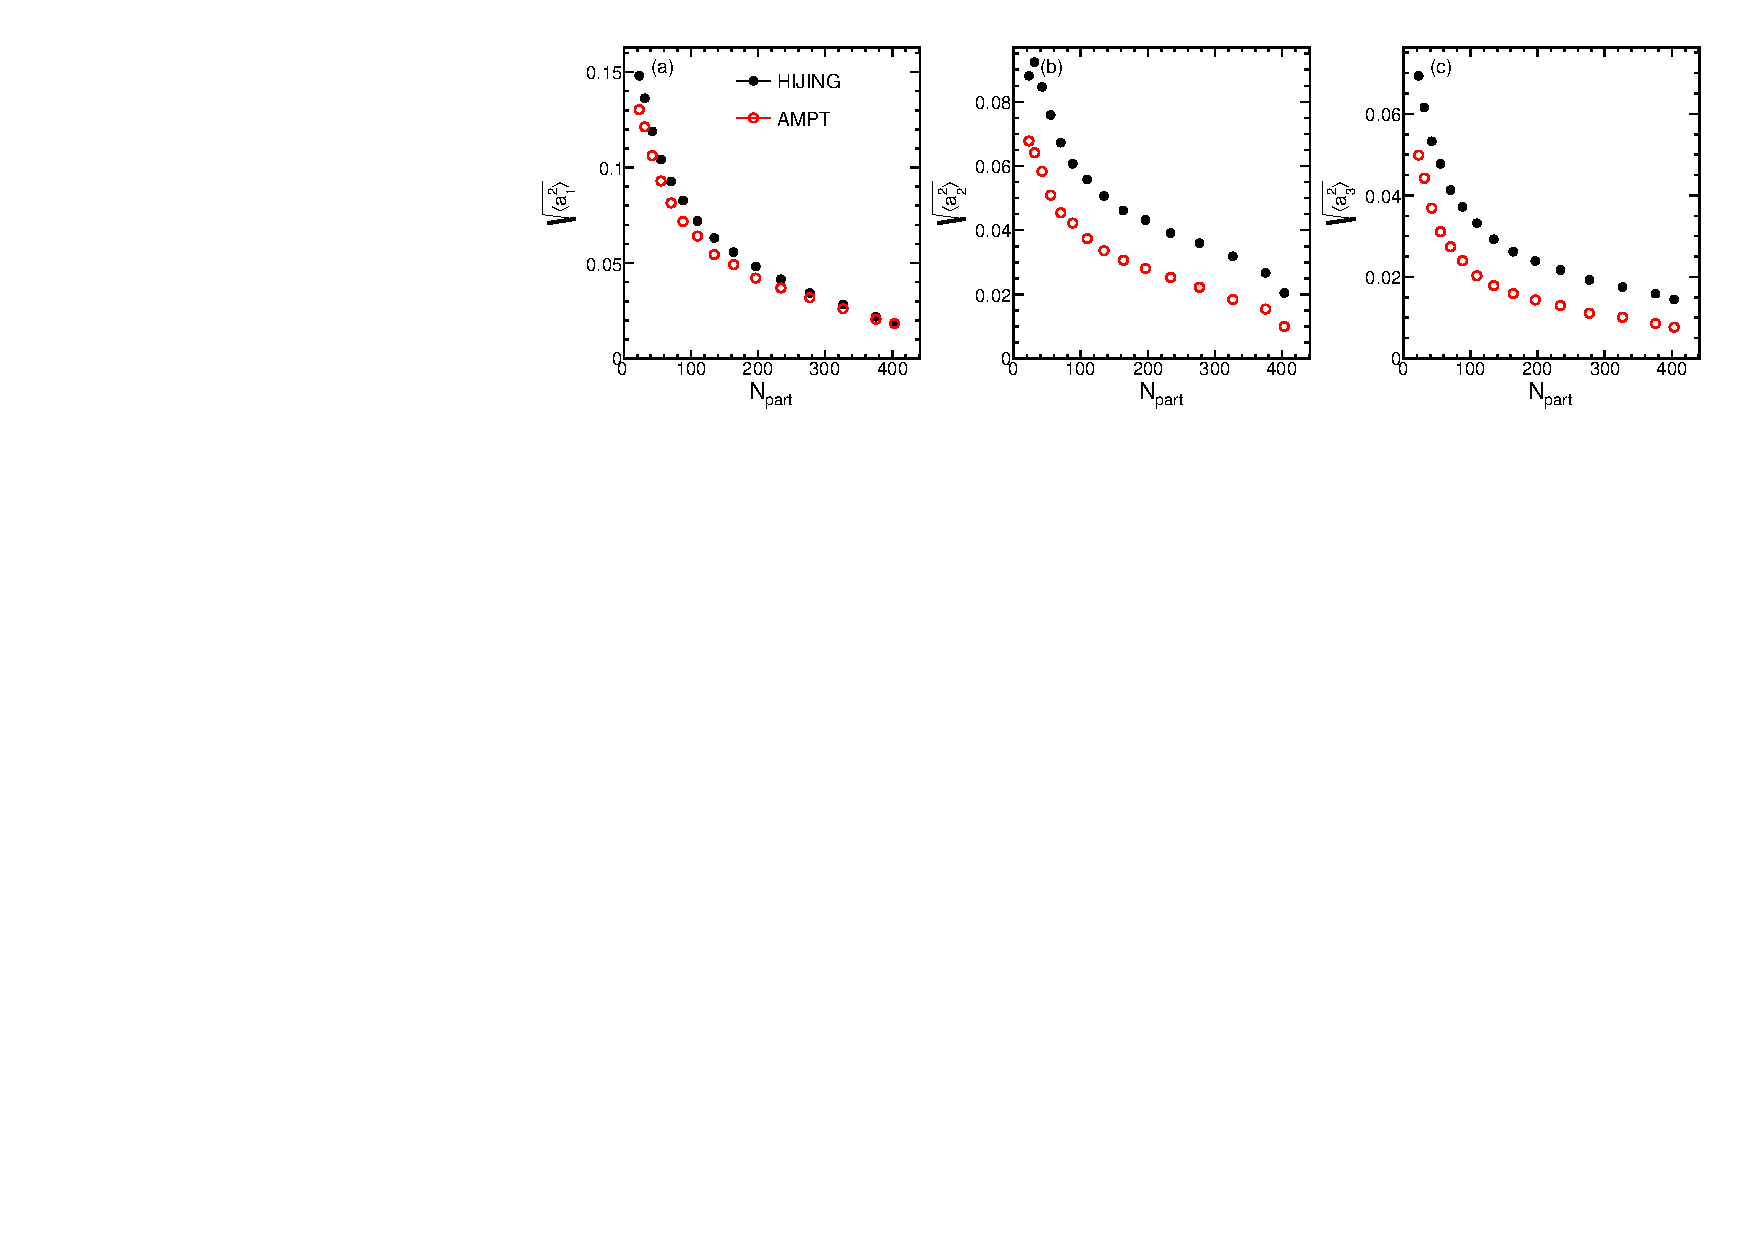
\includegraphics[width=.95\linewidth]{figs/chapter_fbcorr/Model_an.pdf}
\caption{Centrality dependence of $a_1$ (left), $a_2$ (middle) and $a_3$ (right) for HIJING and AMPT events.}
\label{fig:fbcorr_Model_an}
\end{figure}

In order to find out whether the FB multiplicity fluctuation is related to the difference between $\Nf$ and $\Nb$, $a_n^\text{obs}$ is correlated directly with $A_\text{part}$, defined as
\begin{equation}
A_\text{part} = \frac{\Nf - \Nb}{\Nf + \Nb}
\end{equation}
The results for impact parameter $b=8$ fm from HIJING events are shown in Figure~\ref{fig:fbcorr_Model_an_Anpart} (results for AMPT events are similar). A strong positive correlation between $a_1^\text{obs}$ and $A_\text{part}$ is observed, suggesting that the FB asymmetry in the multiplicity distribution is indeed driven by the asymmetry in the number of participating nucleons in the two colliding nuclei. A weak correlation is also observed between $a_3^\text{obs}$ and $A_\text{part}$, suggesting that the FB asymmetry caused by $A_\text{part}$ contains a small nonlinear odd component. On the other hand, there is no correlation between $a_2^\text{obs}$ (rapidity even) and $A_\text{part}$ (rapidity odd) as expected. The width of these distributions are partially due to statistical smearing effects in $a_n^\text{obs}$, which can be removed by a 2D unfolding, which we leave for a future work.

\begin{figure}[H]
\centering
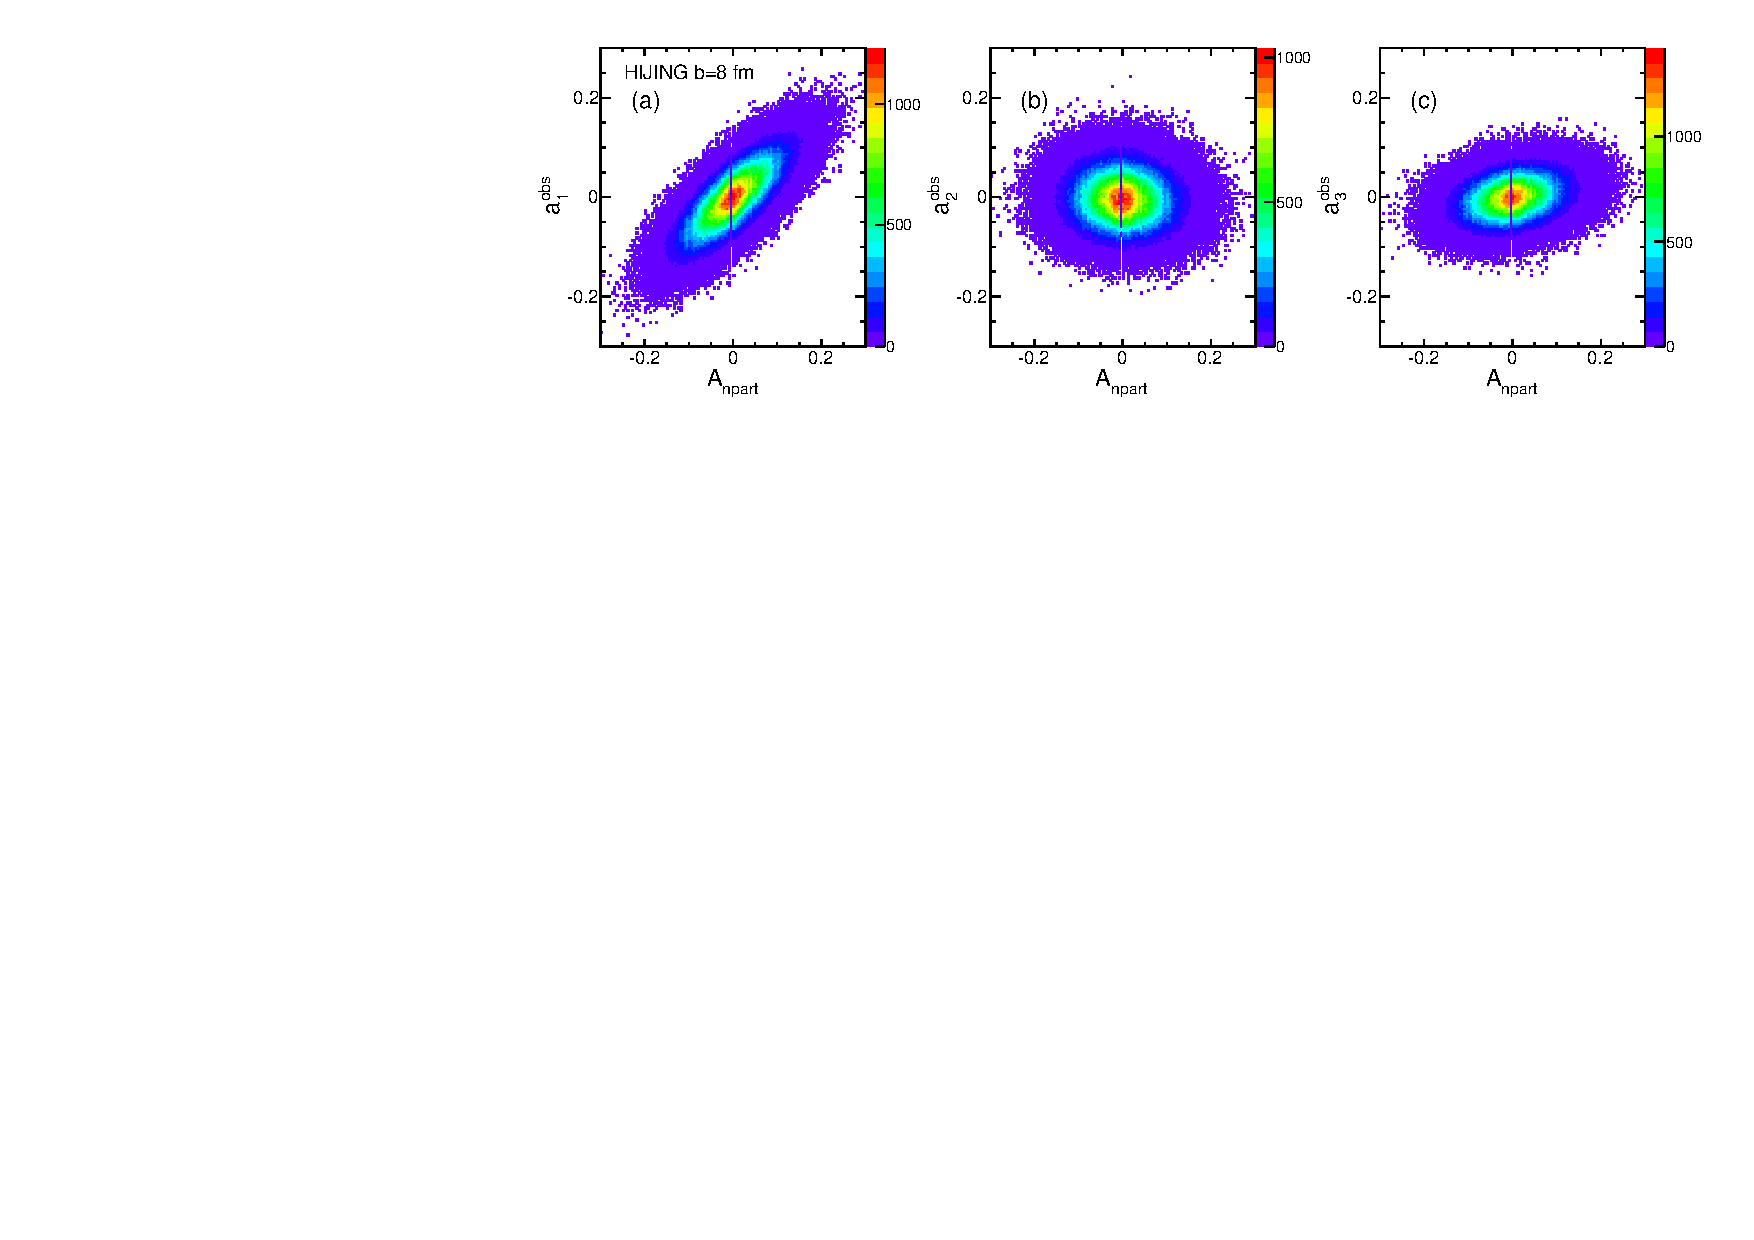
\includegraphics[width=.95\linewidth]{figs/chapter_fbcorr/Model_an_Anpart.pdf}
\caption{Event-by-event correlation between $a_n^\text{obs}$ and $A_\text{part}$ for $n=1$ (left), $n=2$ (middle) and $n=3$ (right) from HIJING events with $b=8$ fm.}
\label{fig:fbcorr_Model_an_Anpart}
\end{figure}

Left panel of Figure~\ref{fig:fbcorr_Model_an_Anpart_comp} compares the centrality dependence of $\sqrt{\lr{a_1^2}}$ and $\sqrt{\lr{A_\text{part}^2}}$. The similarity in their shapes suggests that the asymmetry between $\Nf$ and $\Nb$ is primarily responsible for the FB asymmetry in $N(\eta)$. Note that the FB asymmetry of $R(\eta)$ arising from $a_1$ can be estimated as
\begin{equation}
A_R(\eta) \approx \sqrt{\lr{a_1^2}} T_1(\eta) = \sqrt{\frac{3}{2}}\sqrt{\lr{a_1^2}}\frac{\eta}{6}.
\end{equation}
The results in Figure~\ref{fig:fbcorr_Model_an_Anpart_comp} imply $\sqrt{\lr{a_1^2}} \approx 0.7 \sqrt{\lr{A_\text{part}^2}}$, and hence $A_R(6) \approx 0.86 \sqrt{\lr{A_\text{part}^2}}$. Therefore, the multiplicity fluctuations in the very forward (backward) rapidity $\pm 6$ are mostly driven by the fluctuations in $\Nf$ ($\Nb$). On the other hand, the fluctuation of total multiplicity $M$ is expected to be driven mainly by the fluctuation of $N_\text{part} = \Nf + \Nb$. Given that $a_1$ is driven by $\Nf-\Nb$, the fluctuation of $M$ should not be independent from fluctuation of $a_1$. Right panel of Figure~\ref{fig:fbcorr_Model_an_Anpart_comp} compares the relative multiplicity fluctuation, $\sigma_M / \lr{M}$, with the fluctuation of number of participants $\sigma_{\Npart} / \lr{\Npart}$. Indeed, the two show very similar centrality dependence after applying a constant scale factor.

\begin{figure}[H]
\centering
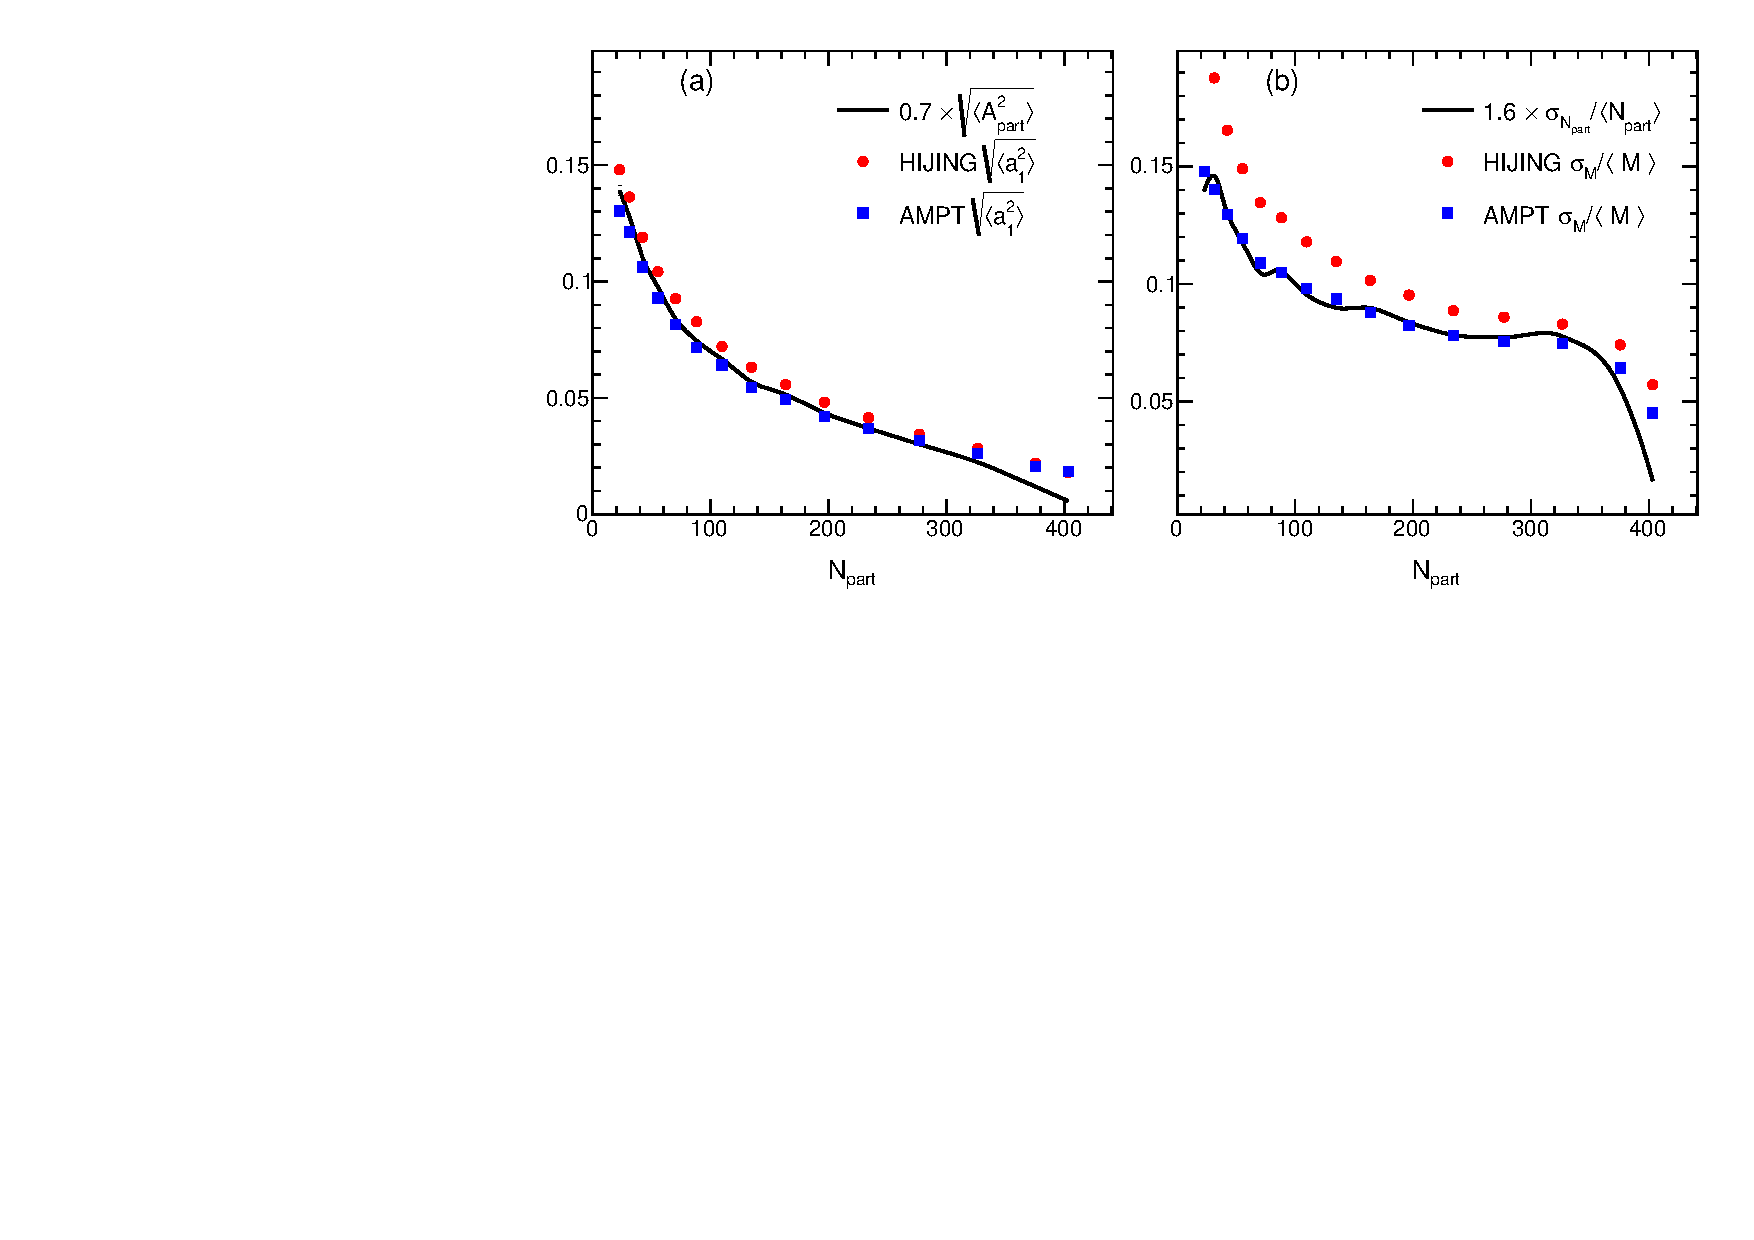
\includegraphics[width=.95\linewidth]{figs/chapter_fbcorr/Model_an_Anpart_comp.pdf}
\caption{Comparison between $\sqrt{\lr{a_n^2}}$ and RMS asymmetry in $\Npart$, $\sqrt{\lr{A_\text{part}^2}}$ (left), as well as between total multiplicity fluctuation in terms of $\sigma_{\Nch} / \lr{\Nch}$ and fluctuation of total $\Npart$}
\label{fig:fbcorr_Model_an_Anpart_comp}
\end{figure}

The results shown so far are obtained by calculating $\lr{N(\eta)}$ in narrow bins of $M$. Figure~\ref{fig:fbcorr_Model_an_cent} compares these with results obtained in narrow slices of $\Npart$ or $b$. This comparison is useful because experiments can only measure $\lr{N(\eta)}$ in finite centrality interval for which the overall multiplicity can still have significant fluctuations. Figure~\ref{fig:fbcorr_Model_an_cent} shows that the values of $a_1$ and $a_3$ have very weak dependence on the averaging scheme, which $a_2$ has rather strong dependence. The latter suggests that a significant component of the $a_2$ obtained for binning in $\Npart$ or $b$ arises from the residual centrality dependence in the shape of $\lr{N(\eta)}$.

\begin{figure}[H]
\centering
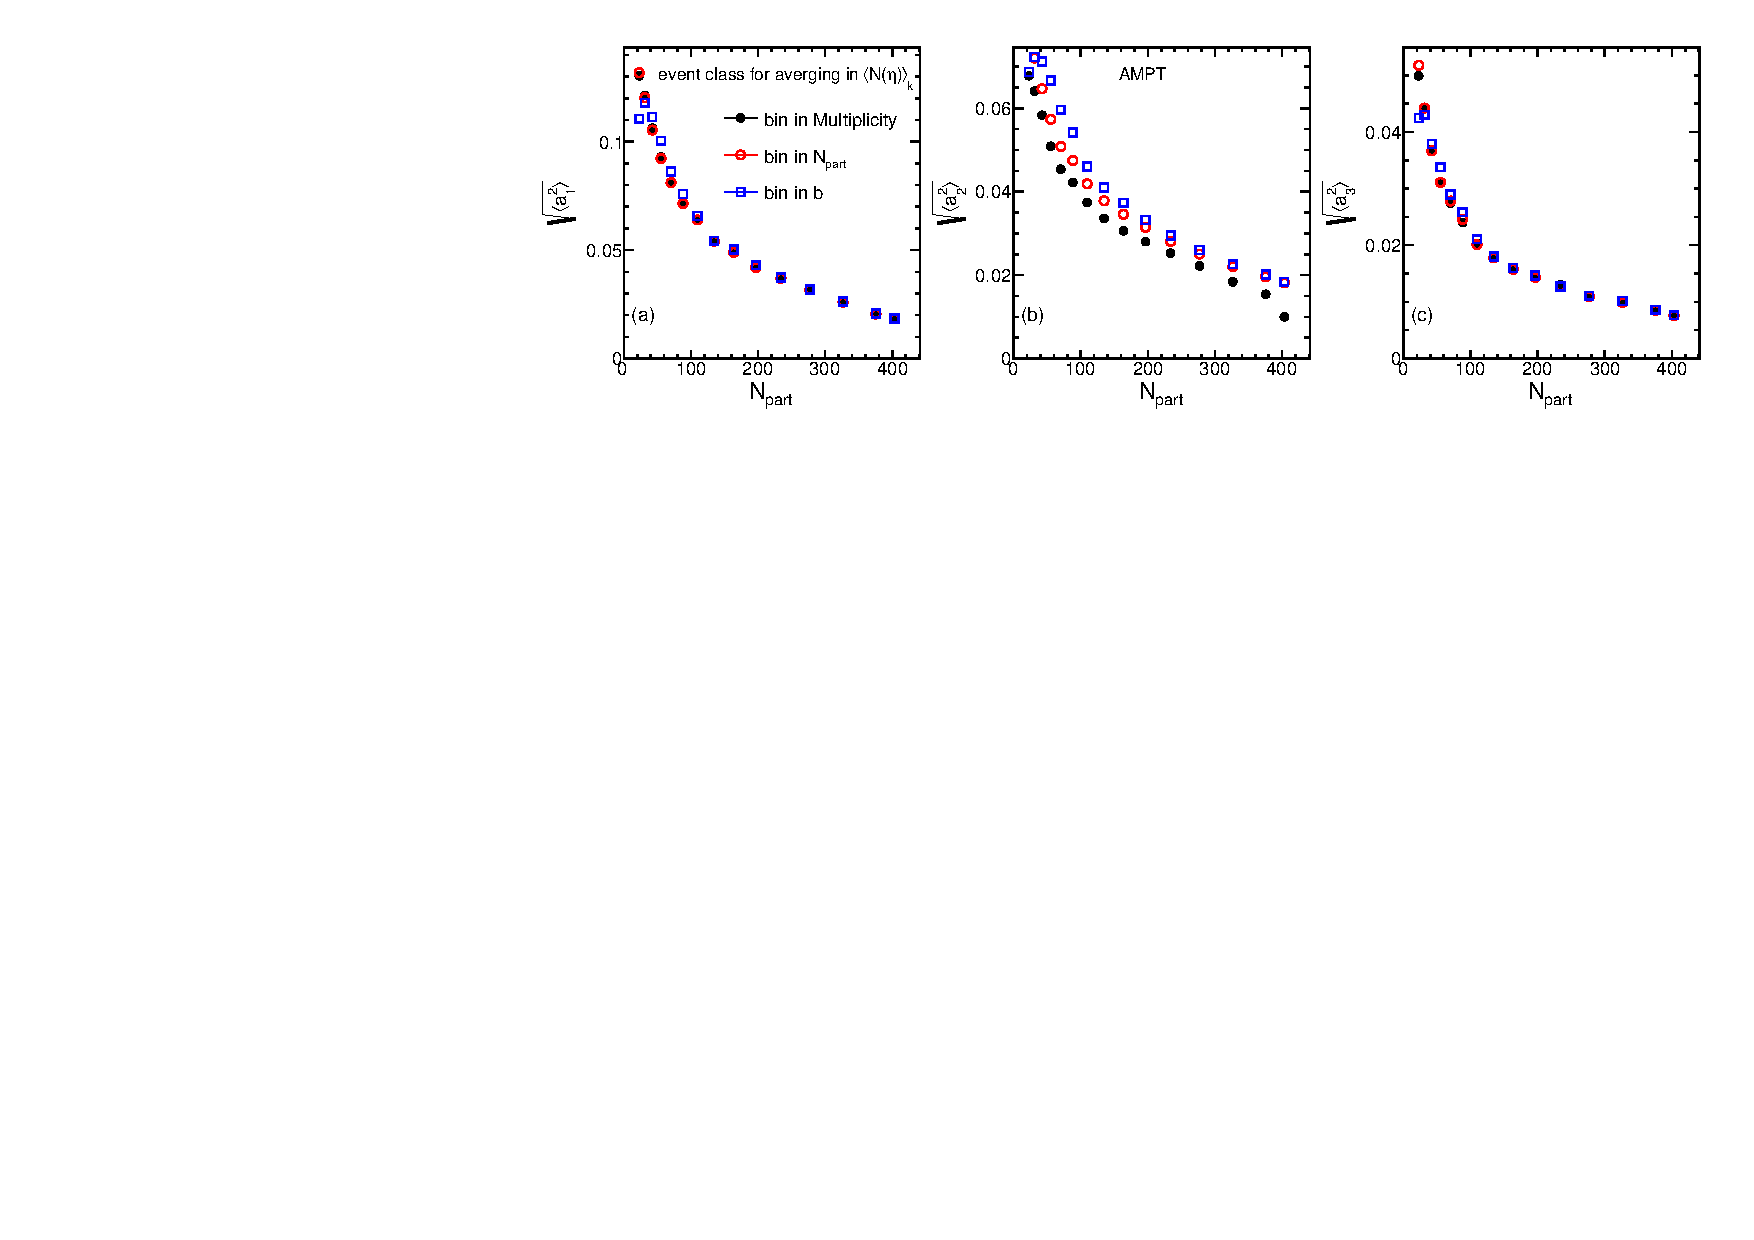
\includegraphics[width=.95\linewidth]{figs/chapter_fbcorr/Model_an_cent.pdf}
\caption{Comparison of the $a_n$ obtained from the three averaging methods, i.e., binning in total multiplicity, $\Npart$ or impact parameter $b$, for $\lr{N(\eta)}$ for $n=1$ (left), $n=2$ (middle) and $n=3$ (right).}
\label{fig:fbcorr_Model_an_cent}
\end{figure}

To see how this residual centrality dependence can arise, Figure~\ref{fig:fbcorr_Model_eg_cent} compares the $\lr{N(\eta)}$ obtained for events in the upper or lower tails of the total multiplicity distribution for all events with $b=8$ fm. The ratios on the right panel show that the shape of $\lr{N(\eta)}$ can still vary significantly for events with the same impact parameter but different $M$, and this variation leads to a significant $a_2$ contribution. Nevertheless, after removing this residual centrality dependence by binning events in narrow $M$ ranges, a significantly $a_2$ still remains. This irreducible $a_2$ could reflect strong EbyE fluctuations in the amount of nuclear stopping or shift of the effective center-of-mass of the collisions~\cite{Steinberg:2007fg, Vovchenko:2013viu}. Similar results are also observed in HIJING events. We will extend the discussion of this centrality fluctuation in Section~\ref{chapter:centfluc}.

\begin{figure}[H]
\centering
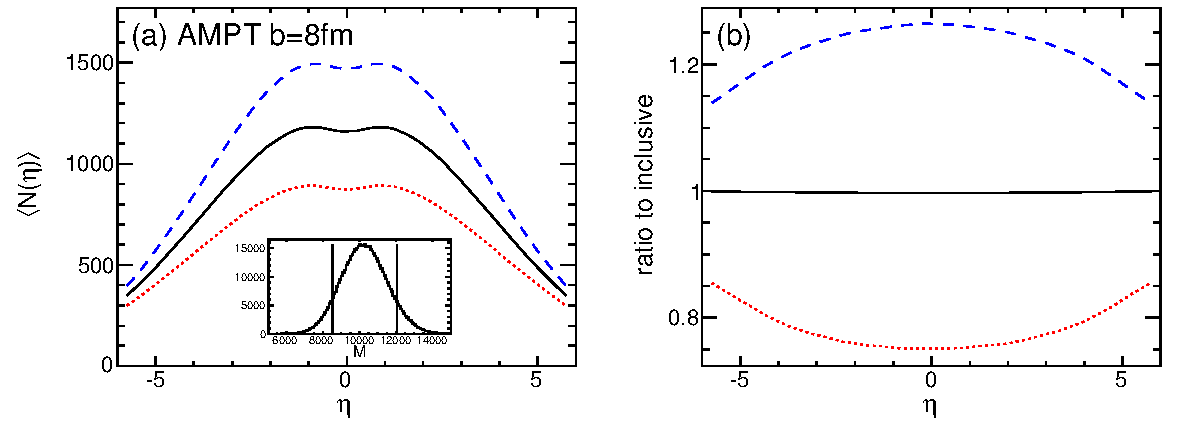
\includegraphics[width=.95\linewidth]{figs/chapter_fbcorr/Model_eg_cent.pdf}
\caption{(a) The average multiplicity distributions for events selected in three multiplicity ranges (see insert) and (b) the ratios to the all events. All events are generated for AMPT model with $b=8$ fm.}
\label{fig:fbcorr_Model_eg_cent}
\end{figure}



\paragraph{Correlating $a_1$ with spectator asymmetry}

If the $a_1$ coefficient is correlated with the fluctuations of $\Nf - \Nb$, then it should be anti-correlated with the asymmetry in the number of spectator nucleons $\Nsf - \Nsb$ since
\begin{equation}
\Nf - \Nb = - (\Nsf - \Nsb).
\end{equation}
The number of spectator nucleons can be measured using calorimeters placed very close to the beamline in the forward region. For example, the ZDC installed in all RHIC and LHC experiments can count the number of spectator neutrons, $N_\text{neu}$, in each event with rather good precision. Unfortunately, the measured neutrons only constitute a small fraction of all spectator nucleons, and hence the correlation between $\Nf - \Nb$ and FB neutron asymmetry $\Nnf - \Nnb$ is expected to be very weak. Nevertheless, studying the correlation between $a_1$ and $\Nsf - \Nsb$ provides an independent and data-driven way for understanding the origin of the FB multiplicity correlations.

Left panel of Figure~\ref{fig:fbcorr_Model_ALICE_neutron} shows the ALICE measurement of the correlation of the ZDC energy with ZEM (forward electromagnetic calorimeter) ($4.8 < |\eta| < 5.7$) energy in Pb+Pb collisions at $\sqrt{s_\text{NN}}=2.76$ TeV~\cite{Abelev:2013qoq}. The latter has a very strong correlation with the Silicon Pixel Detector (SPD) situated in mid-rapidity ($|\eta|<1.9$) as shown by the insert panel. The ZEM signal can be mapped onto the $N_\text{part}$ assuming $E_\text{ZEM} \propto N_\text{part}$, and the ZDC signal is converted to $N_\text{neu}$ from the expected energy for each spectator nucleon of 1.38 TeV: $N_\text{neu} = E_\text{ZDC}/1.38$. From this, the correlation between $N_\text{part}$ and the average number of neutrons $\lr{N_\text{neu}}$ is estimated and shown in the right panel of Figure~\ref{fig:fbcorr_Model_ALICE_neutron}, where the error bars indicate the approximate standard deviations. This correlation is then down-scaled by a factor of two in both axes to give the correlation between $\Nf$ and $\lr{\Nnf}$ or between $\Nb$ and $\lr{\Nnb}$. However, the error bar is reduced only by a factor of $\sqrt{2}$, assuming the sampling of $\Nnf$ is independent of $\Nnb$ once the values of $\Nf$ and $\Nb$ are fixed in each event, hence $\Nsf$ and $\Nsb$ are also fixed. This new distribution is then used to generate the $\Nnf$ and $\Nnb$ for each HIJING or AMPT event based on its $\Nf$ and $\Nb$ values. Finally we calculate the correlation between $\Nnf - \Nnb$ and $a_1^\text{obs}$.

\begin{figure}[H]
\centering
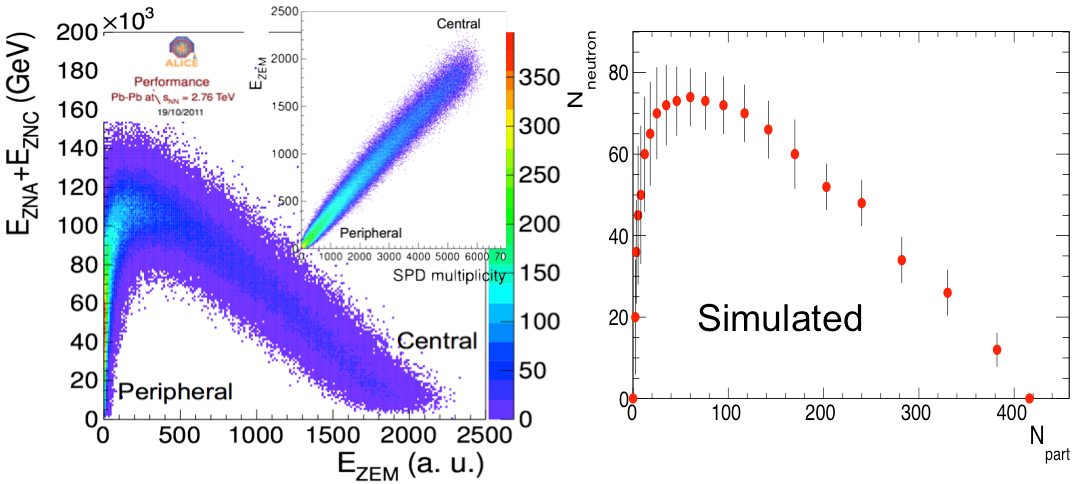
\includegraphics[width=.95\linewidth]{figs/chapter_fbcorr/Model_ALICE_neutron.pdf}
\caption{(a) The correlation of signals in ZDC and ZEM from ALICE experiment; the inset shows the correlation of signals in ZEM and SPD. Then number of neutrons are calculated as $N_\text{neu} = E_\text{ZDC} / 1.38$. (b) The inferred correlation between $N_\text{neu}$ and $\Npart$ used in this study.}
\label{fig:fbcorr_Model_ALICE_neutron}
\end{figure}

The results of this study for AMPT events is summarized in Figure~\ref{fig:fbcorr_Model_neutron_fit}. A clear anti-correlation is seen in mid-central and central collisions. However, the correlation is positive in peripheral collisions, which reflects the fact that the value of $N_\text{neu}$ is positively correlation with $N_\text{part}$ in the peripheral collisions (see Figure~\ref{fig:fbcorr_Model_ALICE_neutron}). This correlation is very weak, $a_1^\text{obs}$ varies by a few percent in the available range of $\Nnf - \Nnb$, but should be measurable in experiments.

\begin{figure}[H]
\centering
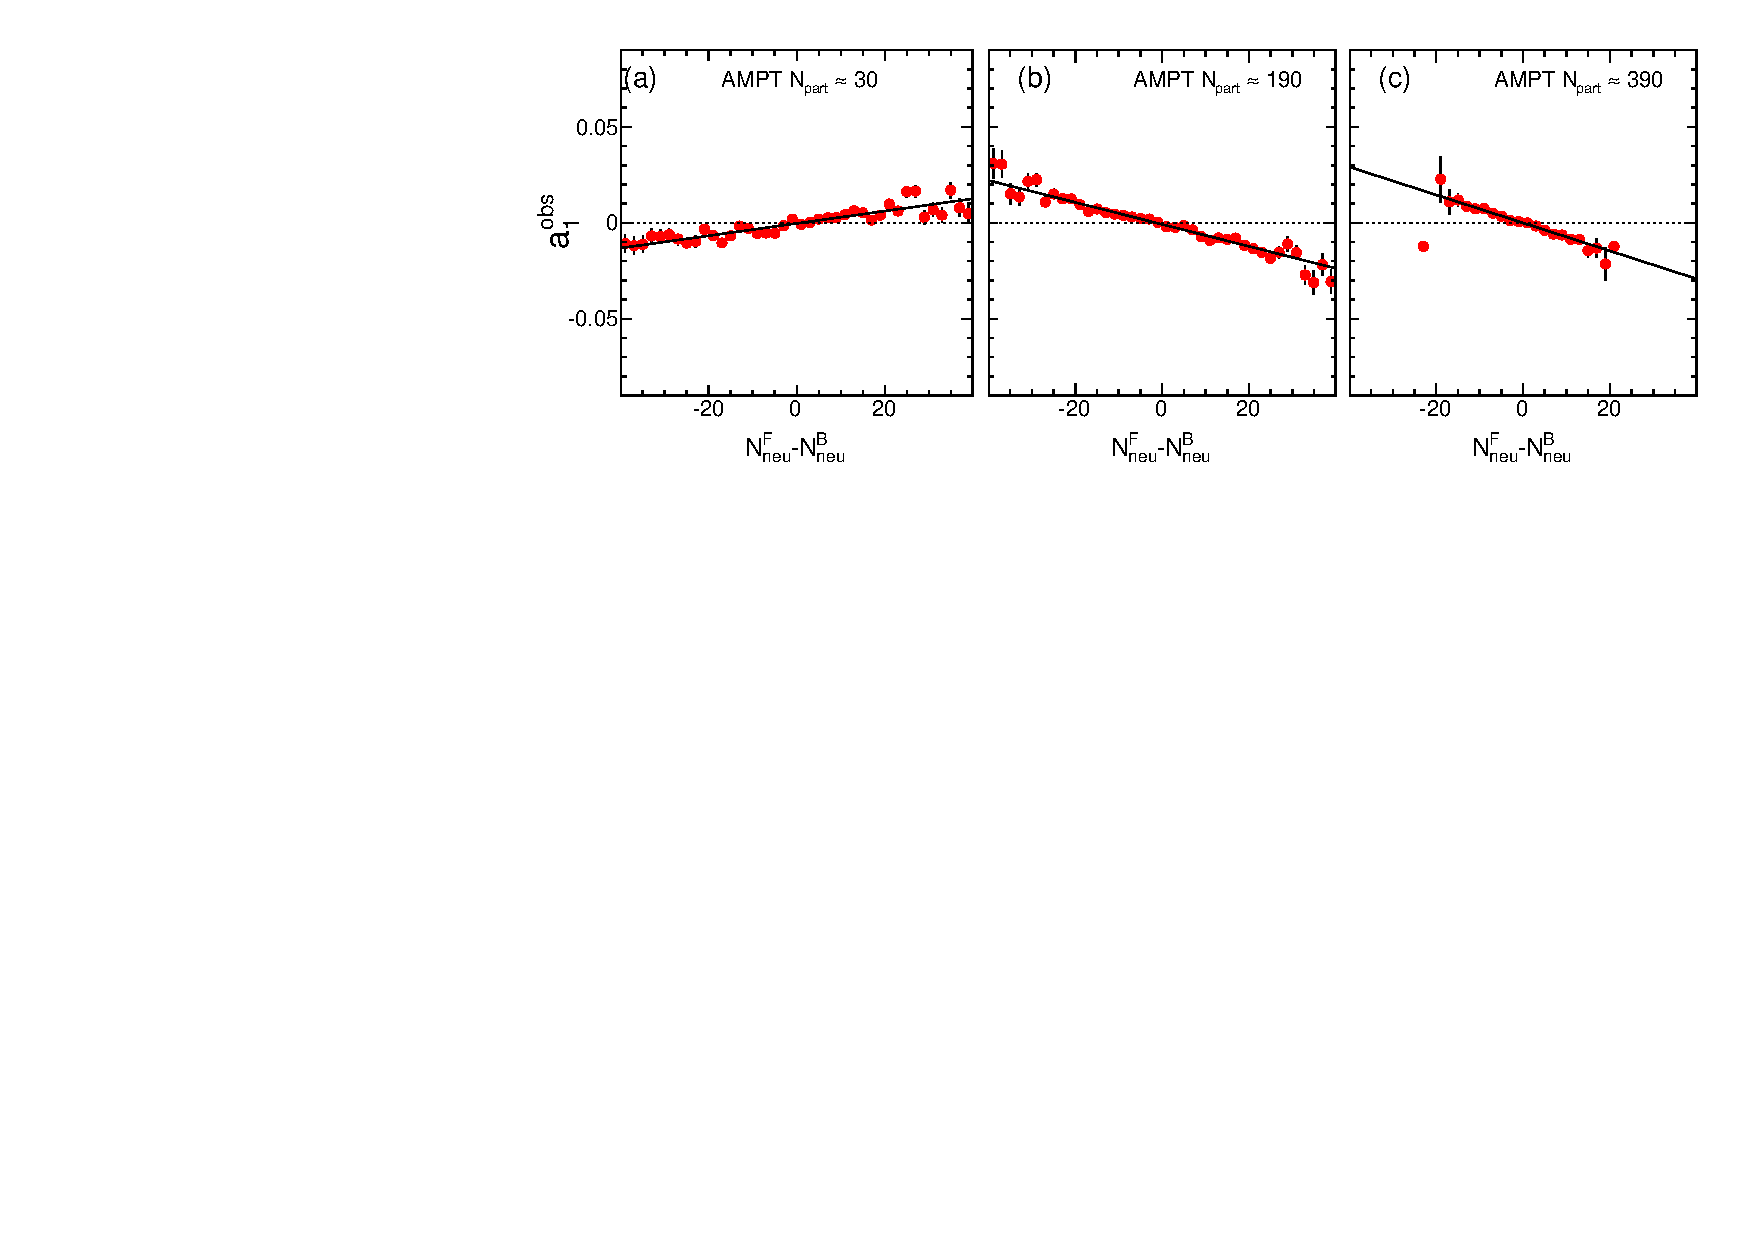
\includegraphics[width=.95\linewidth]{figs/chapter_fbcorr/Model_neutron_fit.pdf}
\caption{The estimated correlation between $a_1^\text{obs}$ and $\Nnf - \Nnb$ for peripheral (left), mid-central (middle) and central (right) Pb+Pb collisions.}
\label{fig:fbcorr_Model_neutron_fit}
\end{figure}



\paragraph{Two-particle correlation method}

As discussed above, $a_n$ coefficients can also be calculated from two-particle correlation method. Left panel of Figure~\ref{fig:fbcorr_Model_1pc_2pc_comp} shows the correlation function and $\lr{a_n a_m}$ values from AMPT events with $b=8$ fm. The shape of the correlation function already suggests the dominance of the $\lr{a_1^2}$ term. The coefficients are compared with those obtained from the single-particle method and identical values are observed. This consistency is expected since the two methods are mathematically equivalent. A selected set of coefficients are shown in the right panel of Figure~\ref{fig:fbcorr_Model_1pc_2pc_comp}. No correlations are observed between the odd and even coefficients as expected for symmetric collision system, while small anti-correlations are observed between odd or event terms, i.e., $\lr{a_n a_{n+2}}<0$ and $\lr{a_n a_{n+4}}<0$.

\begin{figure}[H]
\centering
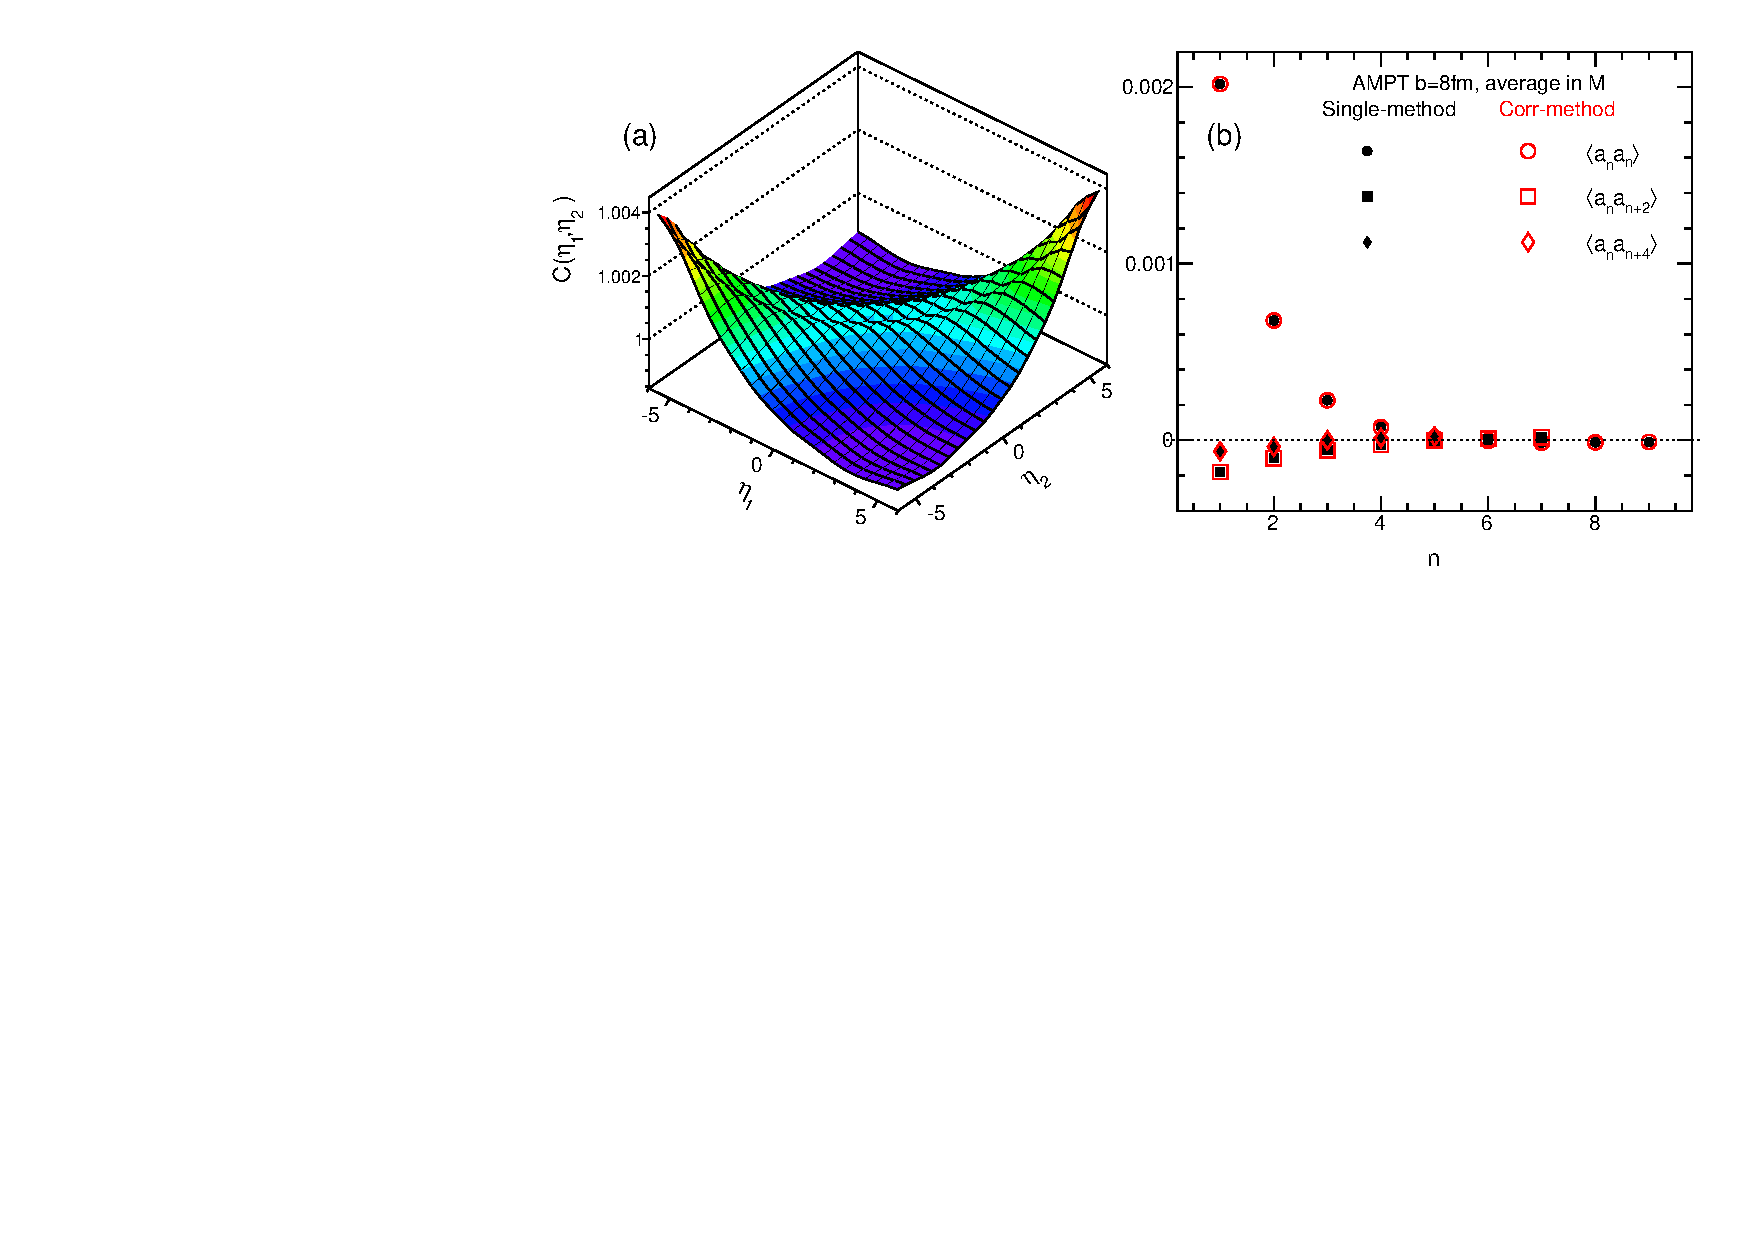
\includegraphics[width=.95\linewidth]{figs/chapter_fbcorr/Model_1pc_2pc_comp.pdf}
\caption{The correlation function (left) and corresponding spectrum $\lr{a_n a_m}$ for $n,m \le 9$ (right) for AMPT events generated with $b=8$ fm, where the $\lr{N(\eta)}$ is calculated in narrow multiplicity bins. The spectrum are compared with those calculated directly from the single-particle method.}
\label{fig:fbcorr_Model_1pc_2pc_comp}
\end{figure}

One important practical advantage of the 2PC method is that it provides a natural way to separate the residual centrality dependence of average shape of $N(\eta)$ from the dynamical shape fluctuations for events with the same centrality:
\begin{equation}
C(\eta_1, \eta_2) = 1 + \frac{1}{2}\lr{a_0 a_0} + \frac{1}{\sqrt{2}}\sum_{n=1}\lr{a_0 a_n}[T_n(\eta1) + T_n(\eta_2)] + \sum_{n,m=1} \lr{a_n a_m}T_n(\eta_1)T_m(\eta_2).
\end{equation}
The first term $\lr{a_0 a_0}$ reflects the multiplicity fluctuation in the given event class, which drops out from the expression if $C(\eta_1, \eta_2)$ is normalized to have a mean value of one, which we shall assume in the following discussion. The second term represents residual centrality dependence in the shape of $\lr{N(\eta)}$. The last term encodes the dynamical shape fluctuations for events with fixed centrality, which can be isolated by dividing the correlation function by its projections on the $\eta_1$ and $\eta_2$ axes:
\begin{equation}
\begin{split}
C_N(\eta_1, \eta_2) &= \frac{C(\eta_1, \eta_2)}{C_p(\eta_1)C_p(\eta_2)}, \\
C_p(\eta_1) &= \frac{\int C(\eta_1, \eta_2) d\eta_2}{2Y}, \\
C_p(\eta_2) &= \frac{\int C(\eta_1, \eta_2) d\eta_1}{2Y}.
\end{split}
\end{equation}
The new correlation function ensures that any residual centrality dependence is taken out from the measured coefficients:
\begin{equation}
C_N(\eta_1, \eta_2) = 1 + \sum_{n,m=1} \lr{a_n a_m} T_n(\eta_1) T_m(\eta_2),
\end{equation}

Figure~\ref{fig:fbcorr_Model_corr_SPM} shows the original correlation function, the product of its projections to the two axes, and the renormalized correlation function for AMPT events for $b=8$ fm, where the average distribution $\lr{N(\eta)}$ is calculated in one bin (as appose to many narrow multiplicity bins then summed as in Figure~\ref{fig:fbcorr_Model_1pc_2pc_comp}). Despite the significant difference in the original correlation function due to the residual centrality dependence, the renormalized correlation function is very similar to that shown in Figure~\ref{fig:fbcorr_Model_1pc_2pc_comp}. The small difference in the four corners of the correlation functions can be attributed to the difference in $\lr{a_2^2}$  between different binning schemes shown in middle panel of Figure~\ref{fig:fbcorr_Model_an_cent}. Thus the $C_N(\eta_1, \eta_2)$ provides a robust way to extract the dynamical shape fluctuations nearly independent of the choice of centrality classes.

\begin{figure}[H]
\centering
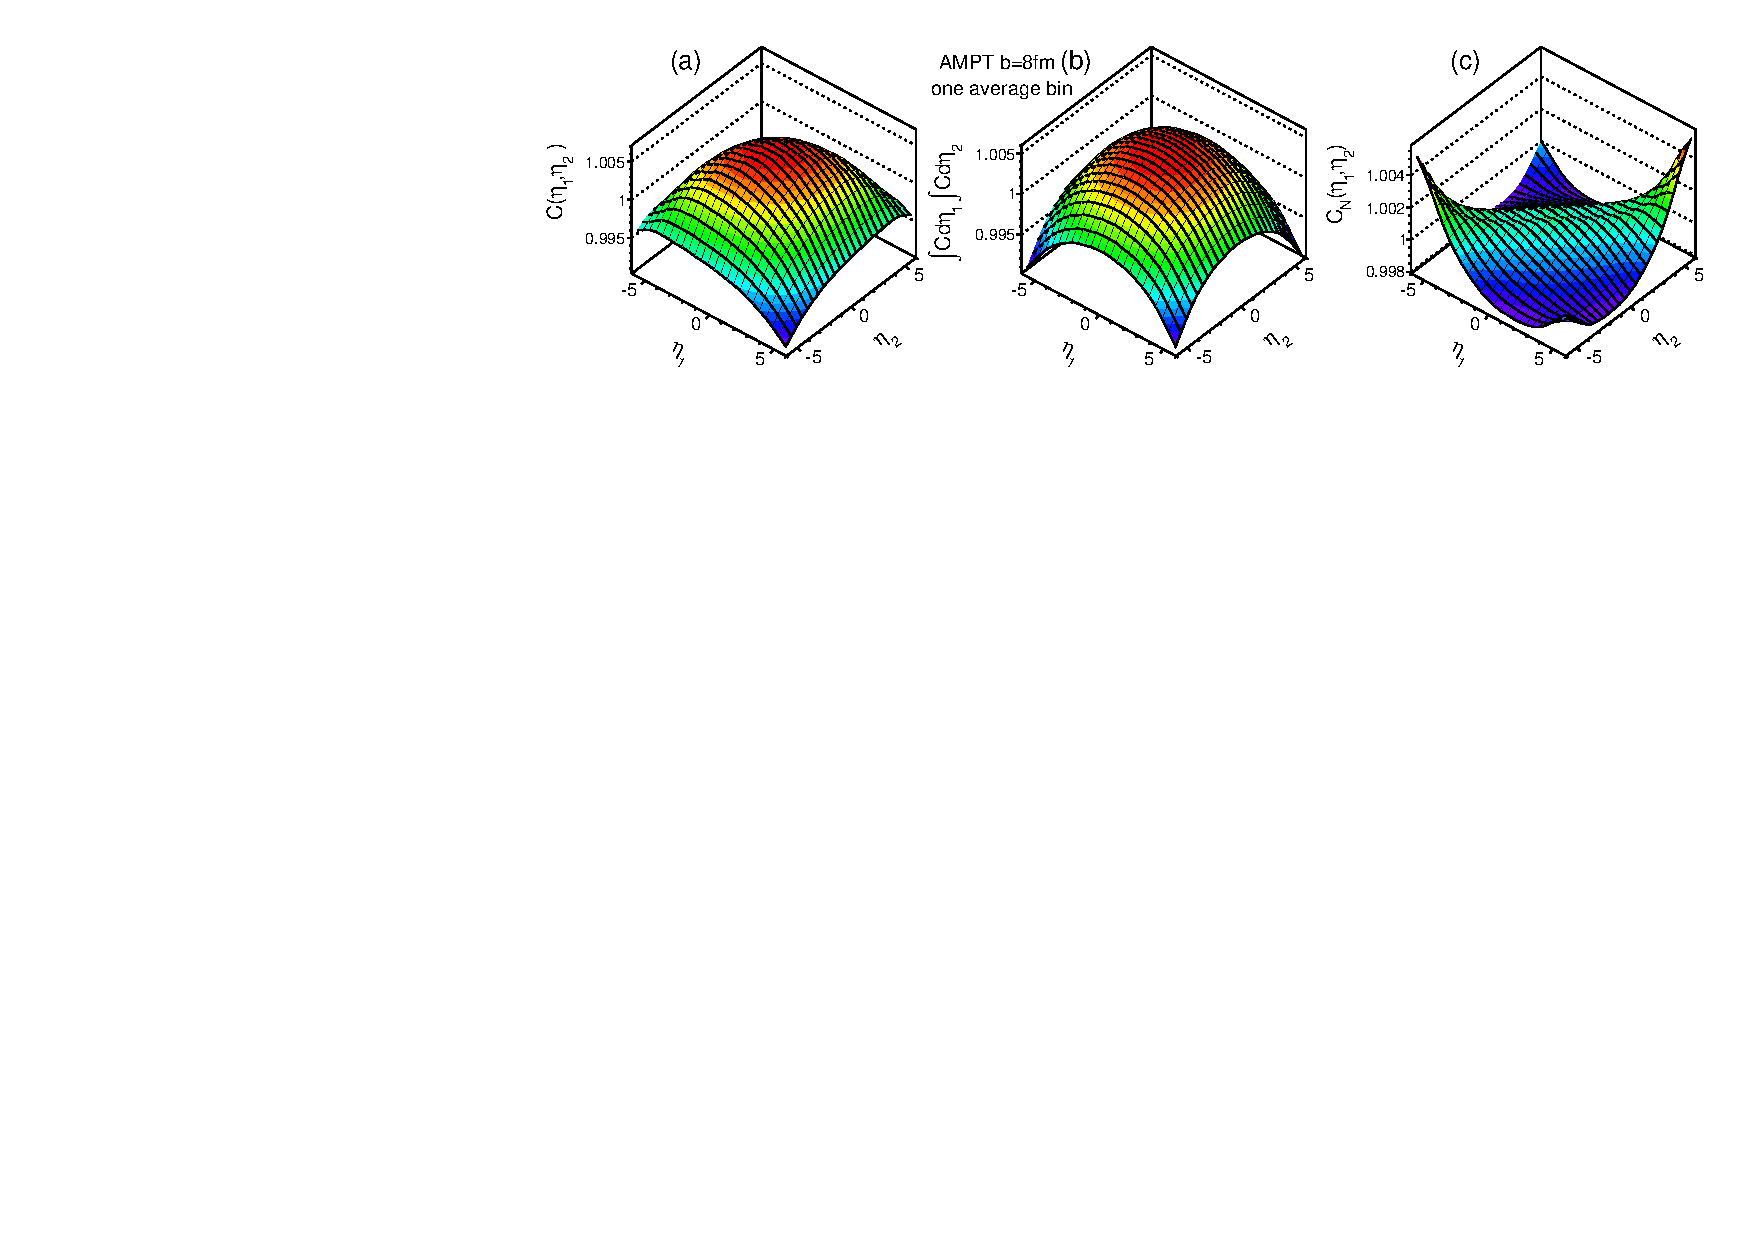
\includegraphics[width=.95\linewidth]{figs/chapter_fbcorr/Model_corr_SPM.pdf}
\caption{The correlation function (left), the product of the projections on two axes (middle) and the redefined correlation function (right) for AMPT events generated with $b=8$ fm. The $\lr{N(\eta)}$ is calculated using all events.}
\label{fig:fbcorr_Model_corr_SPM}
\end{figure}

Figure~\ref{fig:fbcorr_Model_corr_modelComp} compares the correlation functions between the HIJING and AMPT, the correlation function from AMPT appears much broader than the HIJING, which is partially responsible for the faster decrease of the spectrum. The AMPT events also show an interesting shallow minimum around $\delta\eta=0$ with a width of about $\pm 0.4$. Since it is absent in HIJING events, this structure must reflect the influence of the final-state effects implemented in the AMPT model. The correlation function is an intuitive observable for understanding the influence of different underlying physics.

\begin{figure}[H]
\centering
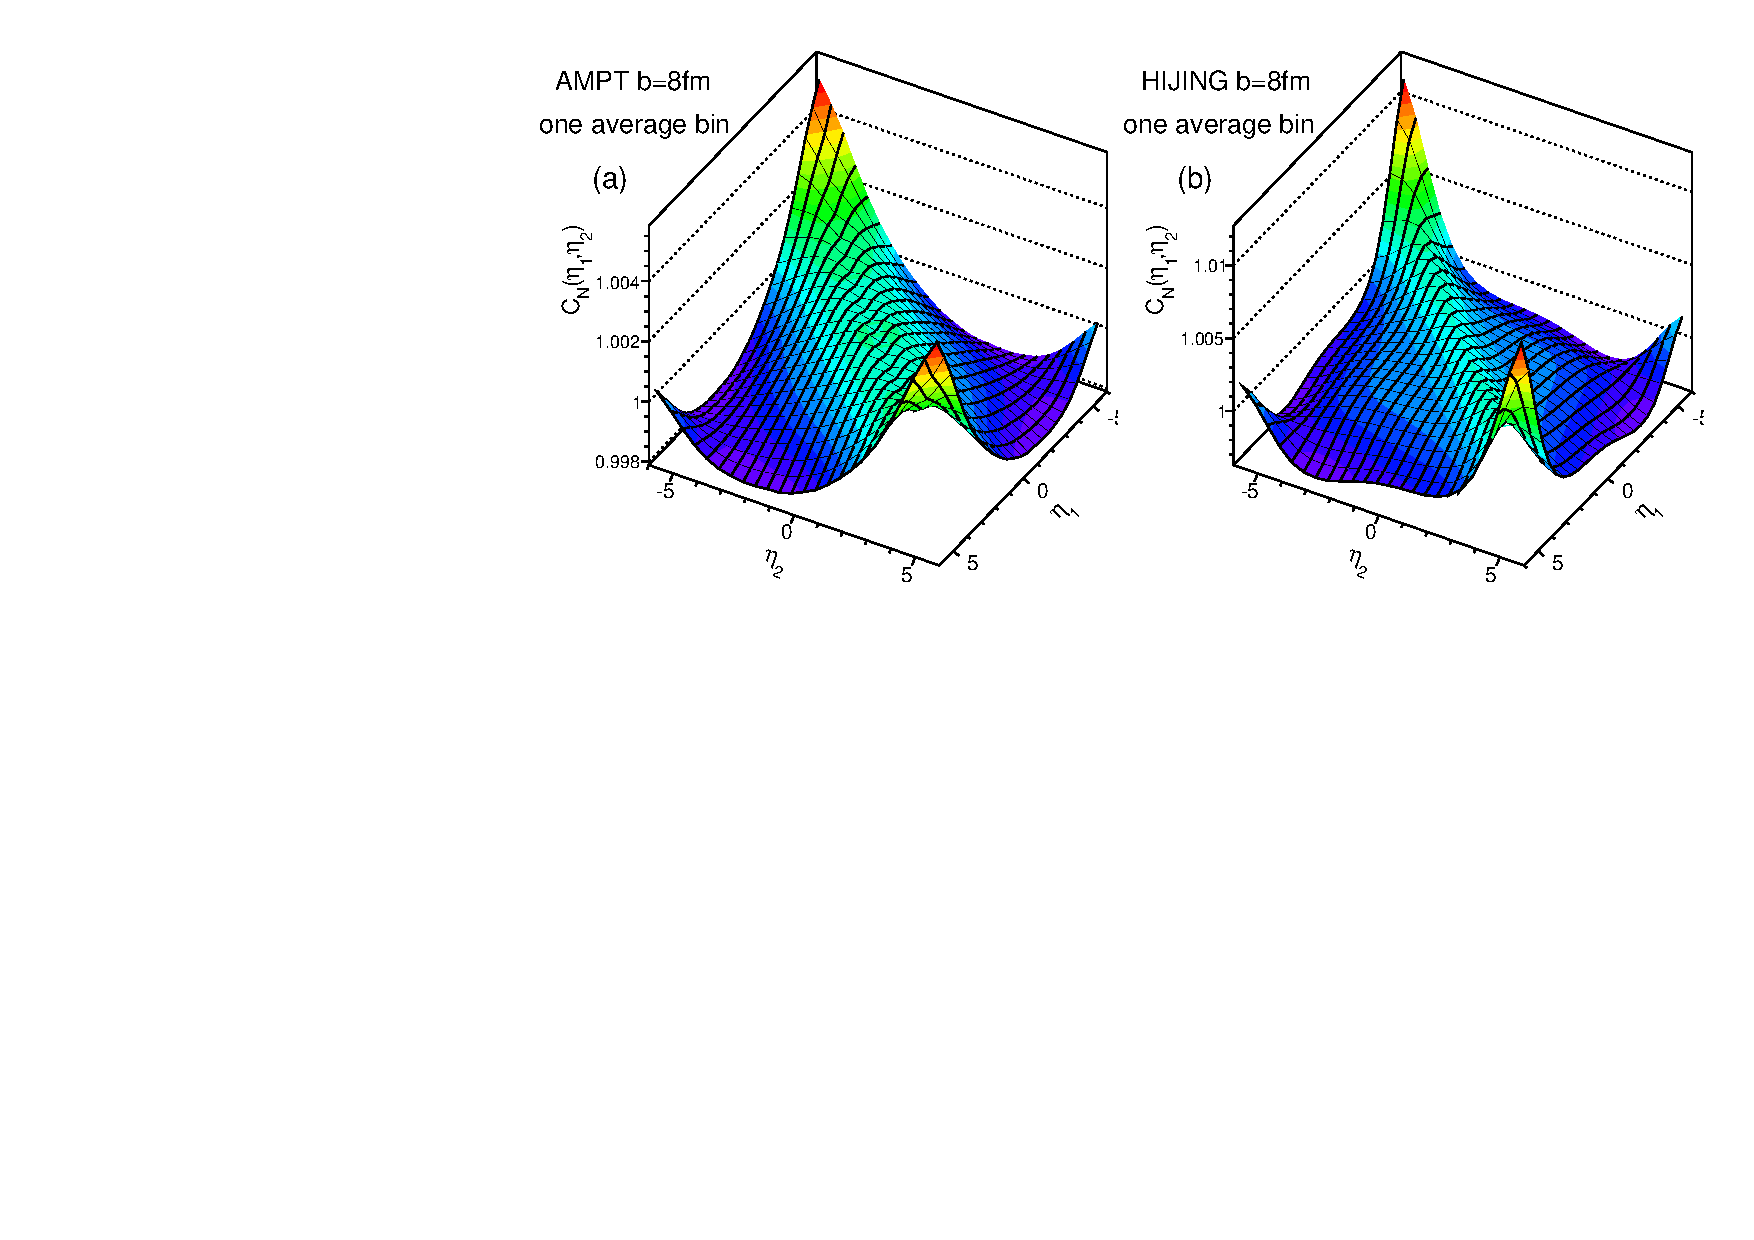
\includegraphics[width=.95\linewidth]{figs/chapter_fbcorr/Model_corr_modelComp.pdf}
\caption{The correlation functions for AMPT (left) and HIJING (right) events generated with $b=8$ fm. The $\lr{N(\eta)}$ is calculated using all events.}
\label{fig:fbcorr_Model_corr_modelComp}
\end{figure}

Note that the correlation function obtained via this procedure is affected by a small bias from short-range component, denoted as $\delta_\text{SRC}(\eta_1, \eta_2)$, via the normalization procedure.  However, the short-range component contribution can be estimated and removed by the iterative procedure discussed above. Therefore $C_N^{'}$ is only corrected for the residual centrality dependence and is free of bias from short-range correlations. One can use $C_N^{'}$ instead of $C_N$ to extract $a_n$ spectra. The main effect of the bias is reduce the values of $C_N$ relative to $C_N^{'}$ at the four corners of the $(\eta_1, \eta_2)$ phase space. We shall leave this topic for the ATLAS data analysis.



\subsubsection{ATLAS data}
\label{sec:fb_atlas_data}

The top row of Figure~\ref{fig:fbcorr_ATLAS_corr_2D} shows the correlation functions $C_N(\eta_1, \eta_2)$ in the three collision systems for events with similar multiplicity $100 \le \Nchrec < 120$. The corresponding estimated SRC component $\delta_\text{SRC}(\eta_1, \eta_2)$ and long-range component $C_N^\text{sub}(\eta_1, \eta_2)$ are shown in the middle and bottom rows, respectively. The magnitude of the SRC in $p$+Pb is observed to be larger in the proton-going direction than in the lead-going direction, reflecting the fact that the particle multiplicity is smaller in the proton-going direction. However, this forward-backward asymmetry in $p$+Pb collisions is mainly associated with the SRC component, and the $C_N^\text{sub}(\eta_1, \eta_2)$ distribution shows very little asymmetry. The $C_N(\eta_1, \eta_2)$ distributions show significant differences between the three systems, which is mainly due to their differences in $\delta_\text{SRC}(\eta_1, \eta_2)$. In fact, the estimated long-range component $C_N^\text{sub}(\eta_1, \eta_2)$ shows similar shape and similar overall magnitude for the three systems.

\begin{figure}[H]
\centering
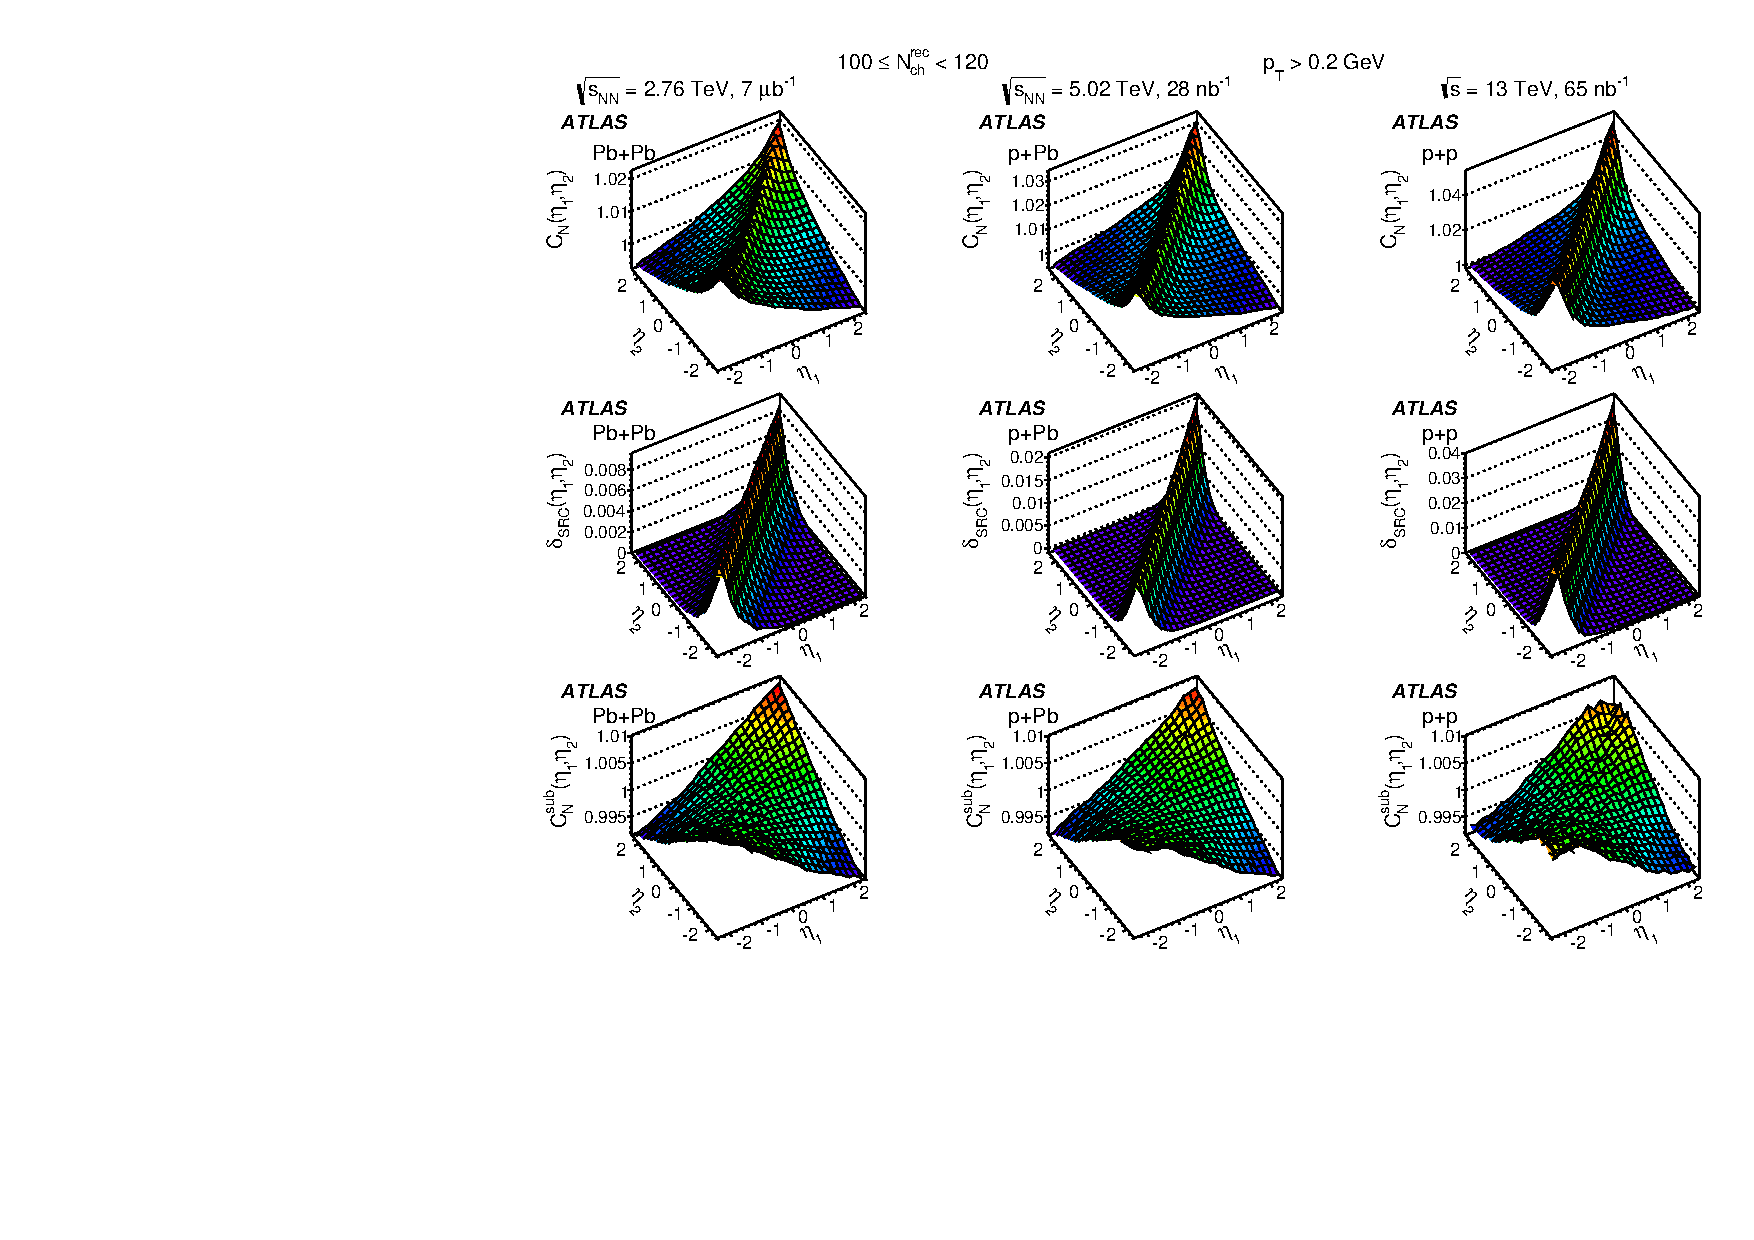
\includegraphics[width=.95\linewidth]{figs/chapter_fbcorr/ATLAS_corr_2D.pdf}
\caption{The distributions of correlation function $C_N(\eta_1, \eta_2)$ (top row), the estimated short-range component $\delta_\text{SRC}(\eta_1, \eta_2)$ (middle row) and long-range component $C_N^\text{sub}(\eta_1, \eta_2)$ (bottom row). They are shown for collisions with $100 \le \Nchrec 120$ in all three collision systems.}
\label{fig:fbcorr_ATLAS_corr_2D}
\end{figure}

To characterize the shape of the correlation functions, the Legendre coefficients $\lr{a_n a_m}$ for the distributions $C_N$ and $C_N^\text{sub}$ shows in Figure~\ref{fig:fbcorr_ATLAS_corr_2D} are calculated and plotted in Figure~\ref{fig:fbcorr_ATLAS_coef}. The $\lr{a_n a_m}$ values are shown for the first six diagonal terms $\lr{a_n^2}$ and the first five mixed terms $\lr{a_n a_{n+2}}$, and they are also compared with coefficients calculated for opposite-charge pairs and same-charge pairs for the same event class. The magnitudes of the $\lr{a_n a_m}$ coefficients calculated for $C_N$ differ significantly for the different charge combinations, and they also increase as the size of the collision system decrease, i.e., $|\lr{a_n a_m}|_{pp} > |\lr{a_n a_m}|_{p\text{+Pb}} > |\lr{a_n a_m}|_\text{Pb+Pb}$ . This is consistent with a large contribution from SRC to all $\lr{a_n a_m}$ coefficients obtained from $C_N$. After removal of the SRC, the $\lr{a_1^2}$ coefficient is quite consistent between different charge combinations and different collision systems. All higher-order coefficients are much smaller, and they are very close to zero within the systematic uncertainties. Therefore, the rest of the discussions focus on the $\sqrt{\lr{a_1^2}}$ results.

\begin{figure}[H]
\centering
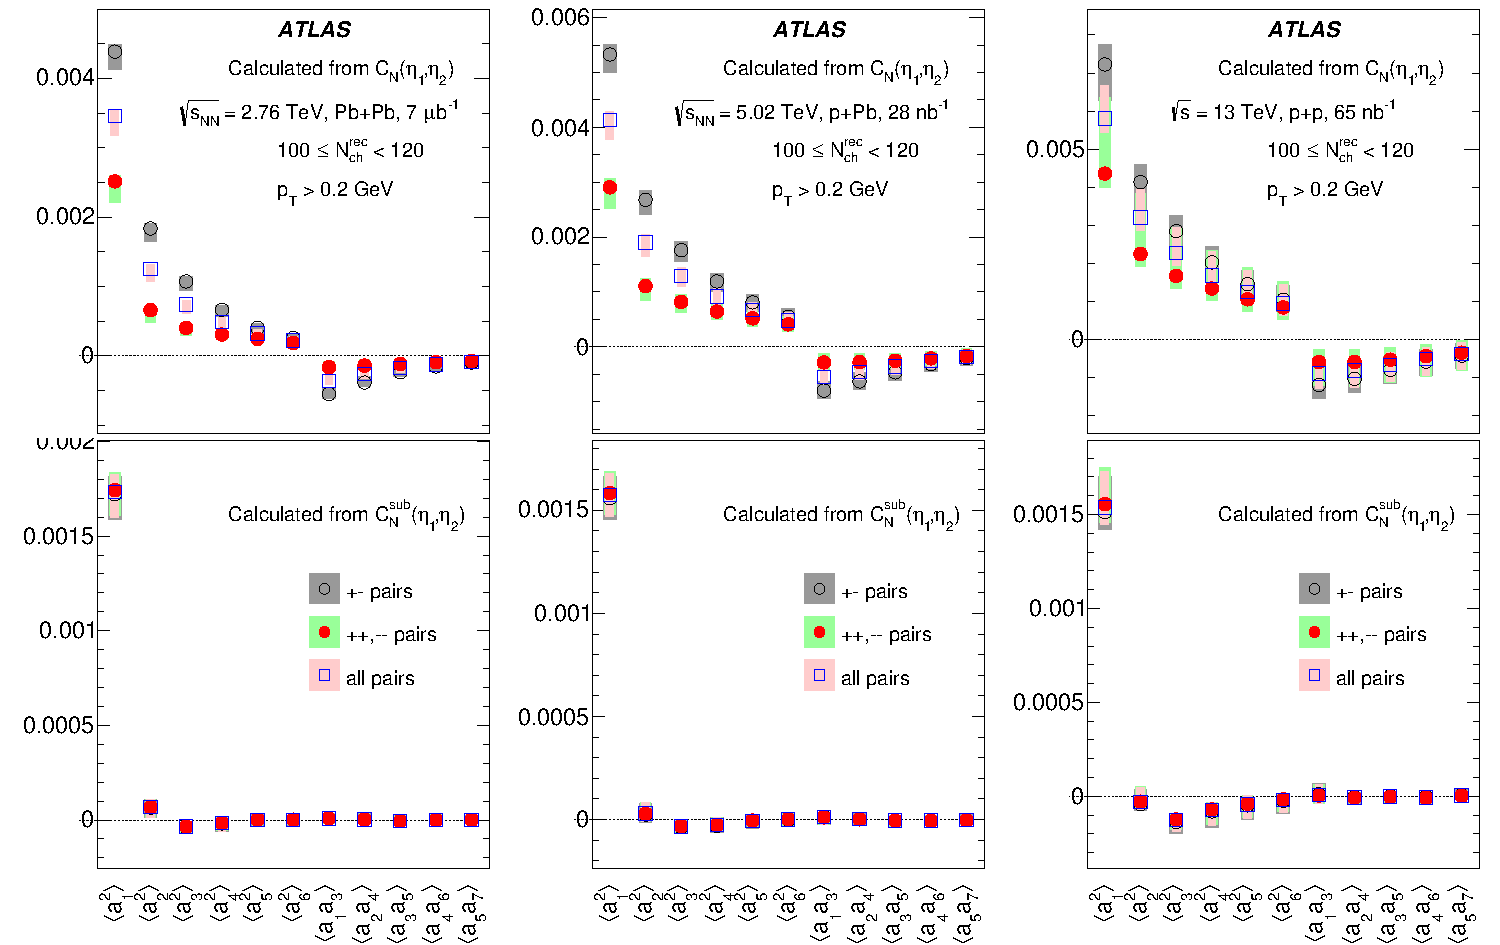
\includegraphics[width=.95\linewidth]{figs/chapter_fbcorr/ATLAS_coef.pdf}
\caption{The Legendre spectra $\lr{a_n^2}$ and $\lr{a_n a_{n+2}}$ calculated from correlation functions $C_N(\eta_1, \eta_2)$ and $C_N^\text{sub}(\eta_1, \eta_2)$ (bottom row) in Pb+Pb (left column), $p$+Pb (middle column) and $pp$ (right column) collisions for events with $100 \le \Nchrec < 120$. The shaded bands represent the total uncertainties.}
\label{fig:fbcorr_ATLAS_coef}
\end{figure}

To quantify further the shape of the LRC in $C_N^\text{sub}(\eta_1, \eta_2)$, the $\sqrt{\lr{a_1^2}}$ coefficients are also calculated by fitting the 1D distributions from the three projection methods as discussed in Section~\ref{sec:fb_other_observables}:
\begin{itemize}
\item quadratic fit of $C_N^\text{sub}(\eta_-)$ in a narrow range of $\eta_+$;
\item quadratic fit of $C_N^\text{sub}(\eta_+)$ in a narrow range of $\eta_-$;
\item linear fit of $r_N^\text{sub}(\eta)$ in a narrow range of $\eta_\text{ref}$.
\end{itemize}
The results for Pb+Pb collisions with $100 \le \Nchrec < 120$ are shown in the first row of Figure~\ref{fig:fbcorr_ATLAS_proj_PbPb} for several selected projections and associated fits. The extracted $\sqrt{\lr{a_1^2}}$ values are shown in the bottom row as a function of the range of the projections. They are compared with the $\sqrt{\lr{a_1^2}}$ values obtained directly via the Legendre expansion of the entire $C_N^\text{sub}$ distribution, shown by the horizontal solid line. The $\sqrt{\lr{a_1^2}}$ values from all methods are very similar.

\begin{figure}[H]
\centering
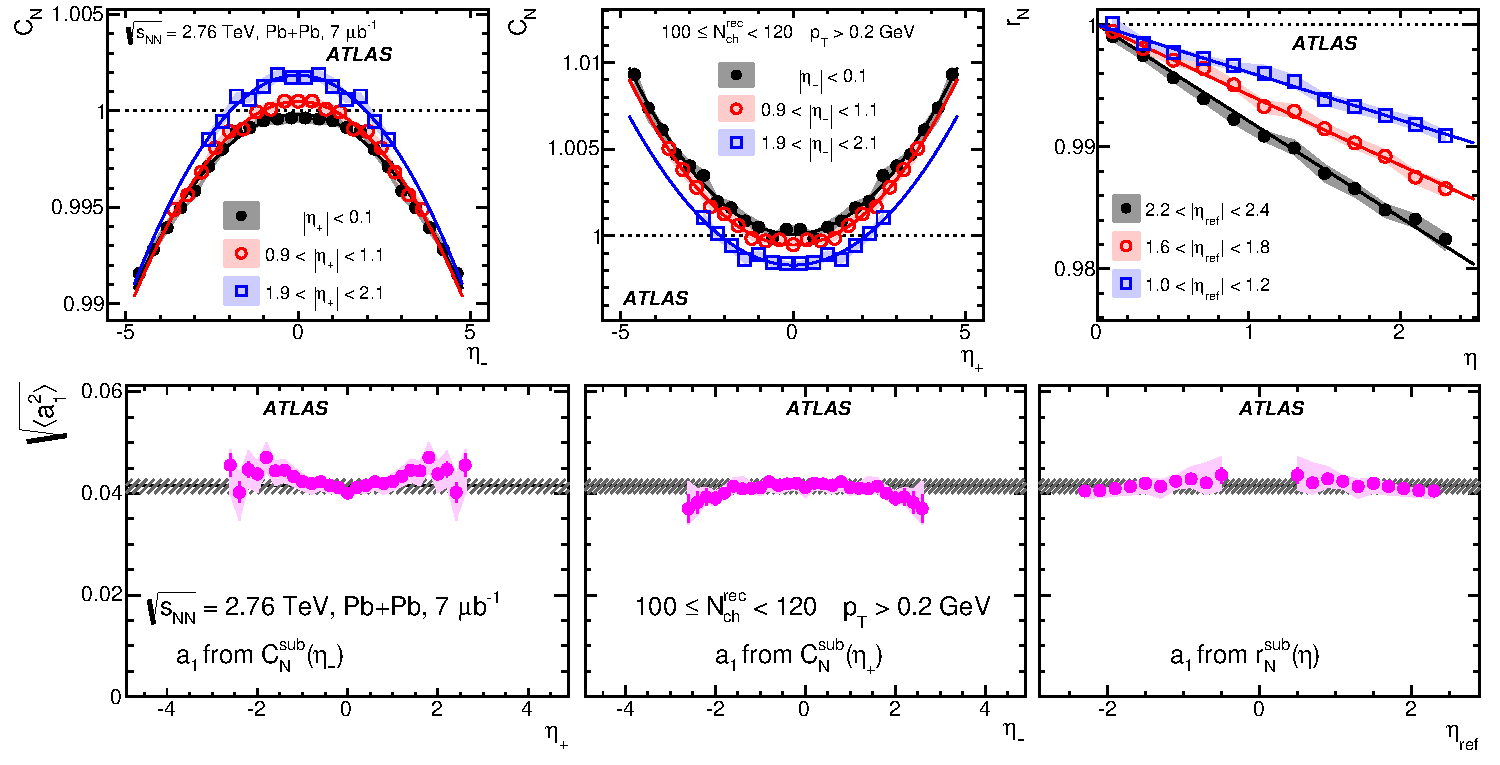
\includegraphics[width=.95\linewidth]{figs/chapter_fbcorr/ATLAS_proj_PbPb.pdf}
\caption{The distributions $C_N^\text{sub}(\eta_-)$ (top left), $C_N^\text{sub}(\eta_+)$ (top middle) and $r_N^\text{sub}(\eta)$ (top right) obtained from $C_N^\text{sub}(\eta_1, \eta_2)$ in three ranges of $\eta_+$, $\eta_-$ and $\eta_\text{ref}$, respectively, from Pb+Pb collisions with $100 \le \Nchrec 120$. The solid lines indicate fits to either a quadratic function or a linear function. The $\sqrt{\lr{a_1^2}}$ values from the fits are shown in the corresponding lower panels as a function of the $\eta_+$, $\eta_-$ and $\eta_\text{ref}$. The solid horizontal line and hashed band indicate the value and uncertainty of $\sqrt{\lr{a_1^2}}$ obtained from a Legendre expansion of the $C_N^\text{sub}(\eta_1, \eta_2)$.}
\label{fig:fbcorr_ATLAS_proj_PbPb}
\end{figure}

Figure~\ref{fig:fbcorr_ATLAS_proj_pPb} and~\ref{fig:fbcorr_ATLAS_proj_pp} show the same observables in $p$+Pb collisions and $pp$ collisions, respectively. Results are quite similar to those in Pb+Pb collisions, albeit with large systematic uncertainties arising from the subtraction of a larger short-range component. For $p$+Pb, the small FB asymmetry in the $C_N^\text{sub}$ distribution along the $\eta_+$ direction is responsible for the difference in the $\sqrt{\lr{a_1^2}}$ between $\eta_+$ and $-\eta_+$ in the bottom left panel and  between $\eta_\text{ref}$ and $-\eta_\text{ref}$ in the bottom right panel, but they still agree within their respective systematic uncertainties.

\begin{figure}[H]
\centering
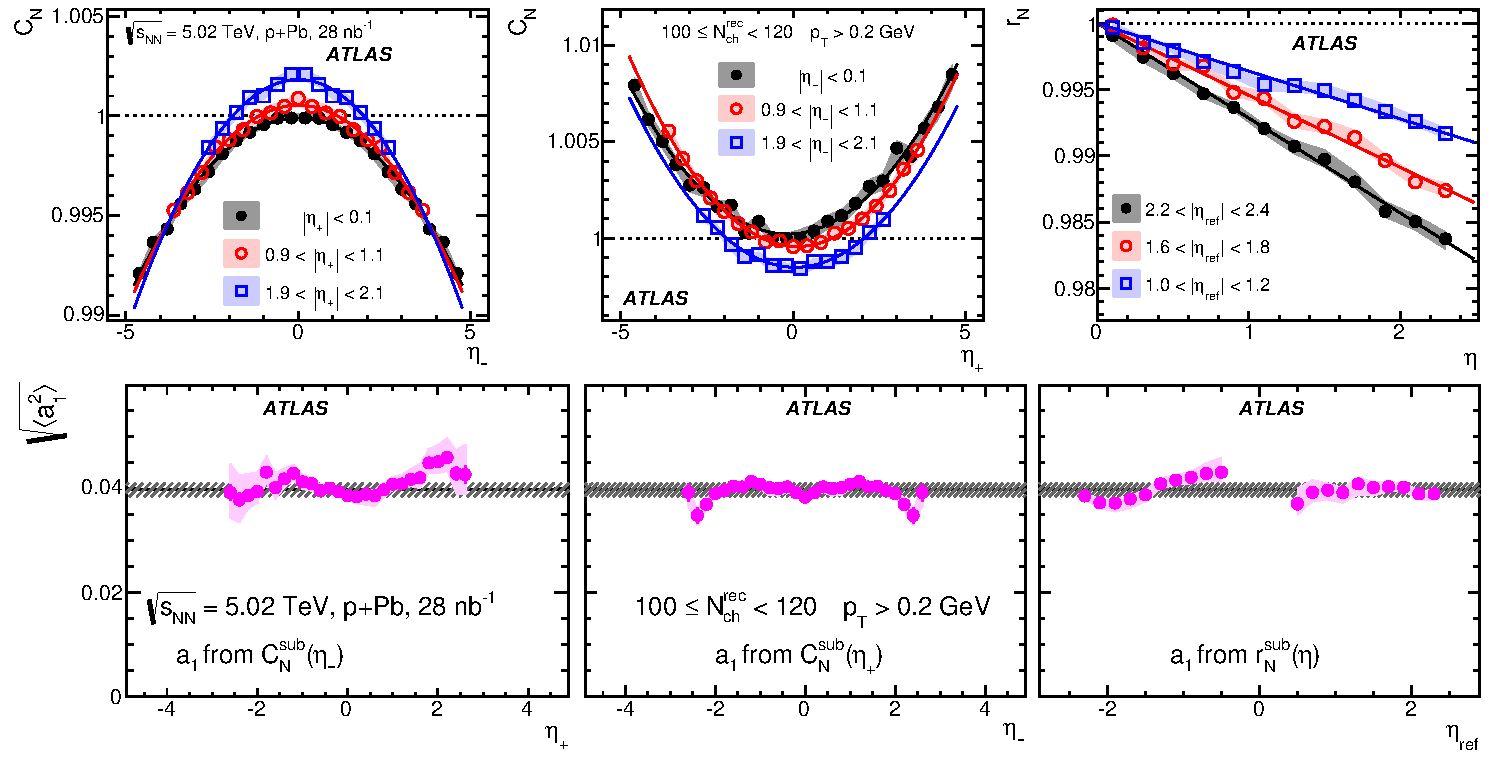
\includegraphics[width=.95\linewidth]{figs/chapter_fbcorr/ATLAS_proj_pPb.pdf}
\caption{The distributions $C_N^\text{sub}(\eta_-)$ (top left), $C_N^\text{sub}(\eta_+)$ (top middle) and $r_N^\text{sub}(\eta)$ (top right) obtained from $C_N^\text{sub}(\eta_1, \eta_2)$ in three ranges of $\eta_+$, $\eta_-$ and $\eta_\text{ref}$, respectively, from $p$+Pb collisions with $100 \le \Nchrec 120$. The solid lines indicate fits to either a quadratic function or a linear function. The $\sqrt{\lr{a_1^2}}$ values from the fits are shown in the corresponding lower panels as a function of the $\eta_+$, $\eta_-$ and $\eta_\text{ref}$. The solid horizontal line and hashed band indicate the value and uncertainty of $\sqrt{\lr{a_1^2}}$ obtained from a Legendre expansion of the $C_N^\text{sub}(\eta_1, \eta_2)$.}
\label{fig:fbcorr_ATLAS_proj_pPb}
\end{figure}

\begin{figure}[H]
\centering
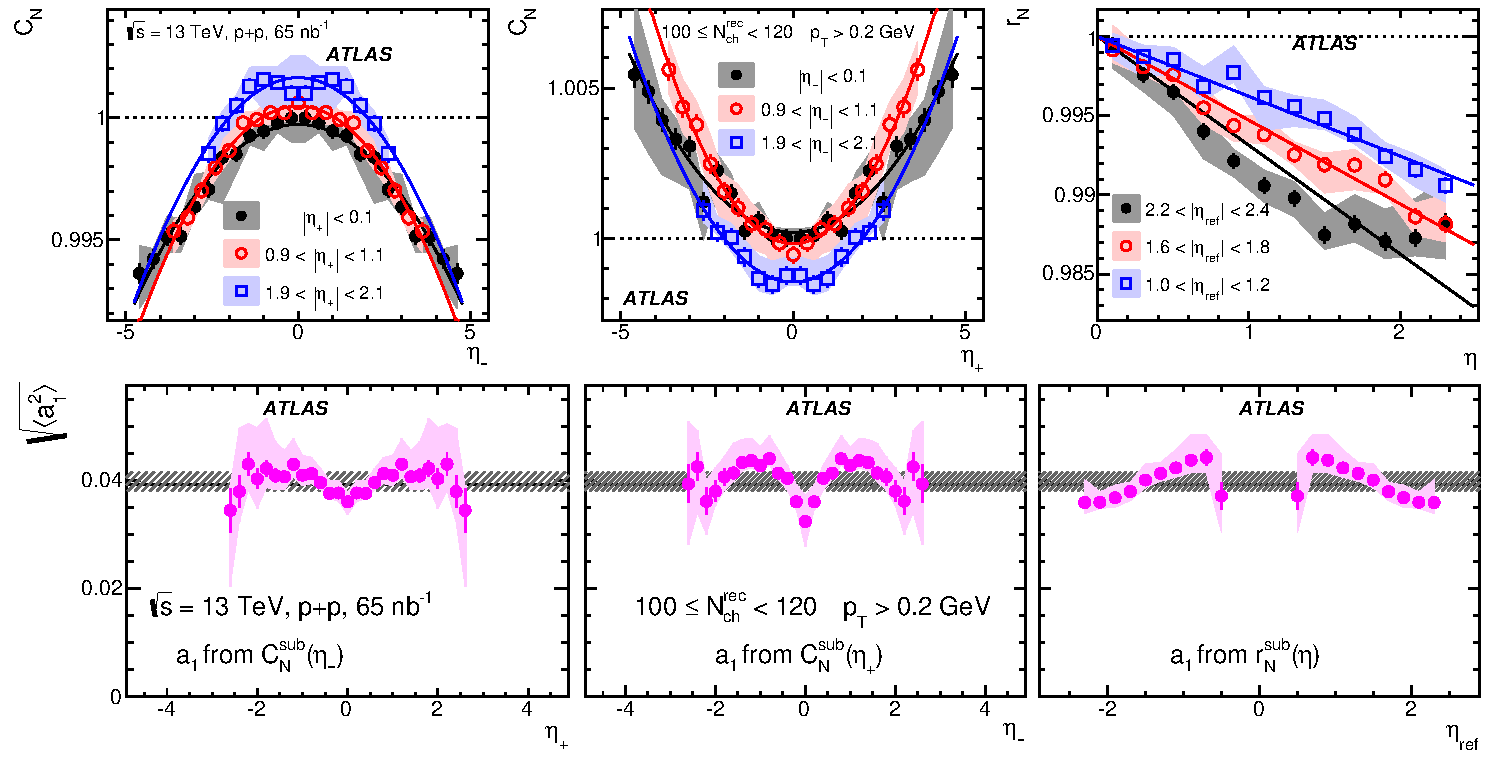
\includegraphics[width=.95\linewidth]{figs/chapter_fbcorr/ATLAS_proj_pp.pdf}
\caption{The distributions $C_N^\text{sub}(\eta_-)$ (top left), $C_N^\text{sub}(\eta_+)$ (top middle) and $r_N^\text{sub}(\eta)$ (top right) obtained from $C_N^\text{sub}(\eta_1, \eta_2)$ in three ranges of $\eta_+$, $\eta_-$ and $\eta_\text{ref}$, respectively, from $pp$ collisions with $100 \le \Nchrec 120$. The solid lines indicate fits to either a quadratic function or a linear function. The $\sqrt{\lr{a_1^2}}$ values from the fits are shown in the corresponding lower panels as a function of the $\eta_+$, $\eta_-$ and $\eta_\text{ref}$. The solid horizontal line and hashed band indicate the value and uncertainty of $\sqrt{\lr{a_1^2}}$ obtained from a Legendre expansion of the $C_N^\text{sub}(\eta_1, \eta_2)$.}
\label{fig:fbcorr_ATLAS_proj_pp}
\end{figure}

Figure~\ref{fig:fbcorr_ATLAS_a1_methodComp} shows a comparison of the $\sqrt{\lr{a_1^2}}$ values extracted by the four methods as a function of $\Nch$ in the three collision systems. Good agreement between the different methods is observed.

\begin{figure}[H]
\centering
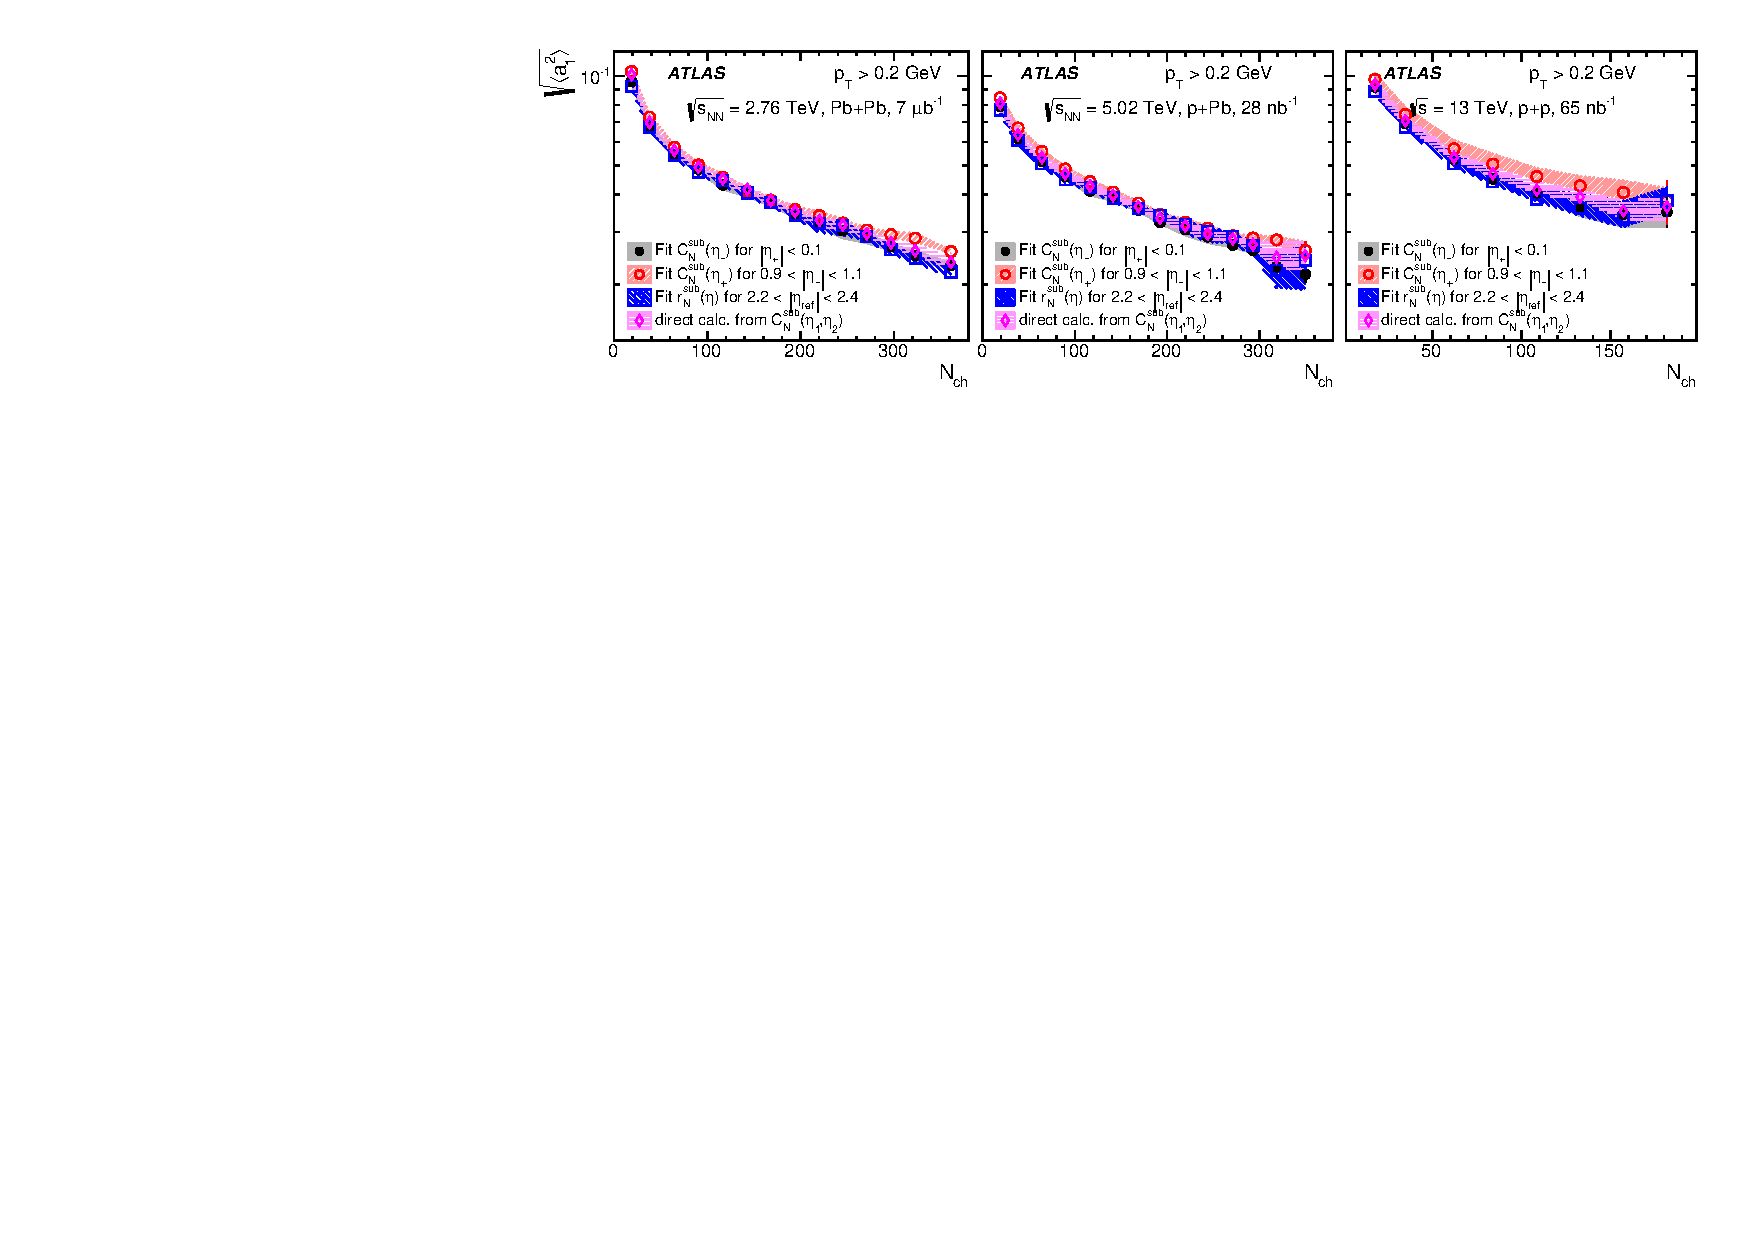
\includegraphics[width=.95\linewidth]{figs/chapter_fbcorr/ATLAS_a1_methodComp.pdf}
\caption{The $\sqrt{\lr{a_1^2}}$ as a function of $\Nch$ from four different methods in Pb+Pb (left), $p$+Pb (middle) and $pp$ (right) collisions. The error bars and shaded bands represent the statistical and systematic uncertainties, respectively.}
\label{fig:fbcorr_ATLAS_a1_methodComp}
\end{figure}

On the other hand, the SRC is expected to have strong dependence on the charge combinations and collision systems, as shown by Figure~\ref{fig:fbcorr_ATLAS_corr_2D} and~\ref{fig:fbcorr_ATLAS_coef}. The magnitude of the SRC is quantified by $\delta_\text{SRC}(\eta_1, \eta_2)$ averaged over the two-particle pseudorapidity phase space:
\begin{equation}
\Delta_\text{SRC} = \frac{\int_{-Y}^Y \delta_\text{SRC}(\eta_1, \eta_2) d\eta_1 d\eta_2}{4Y^2}
\end{equation}
The corresponding distribution of the SRC at the single particle level is $\sqrt{\Delta_\text{SRC}}$, which can be directly compared with the strength of the LRC characterized by $\sqrt{\lr{a_1^2}}$. Figure~\ref{fig:fbcorr_ATLAS_SRC_charge} shows the values of $\sqrt{\Delta_\text{SRC}}$ as a function of $\Nch$ for different charge combinations in the three collision systems. The strength of the SRC always decreases with $\Nch$, and it is larger for smaller collision systems and opposite-charge pairs.

\begin{figure}[H]
\centering
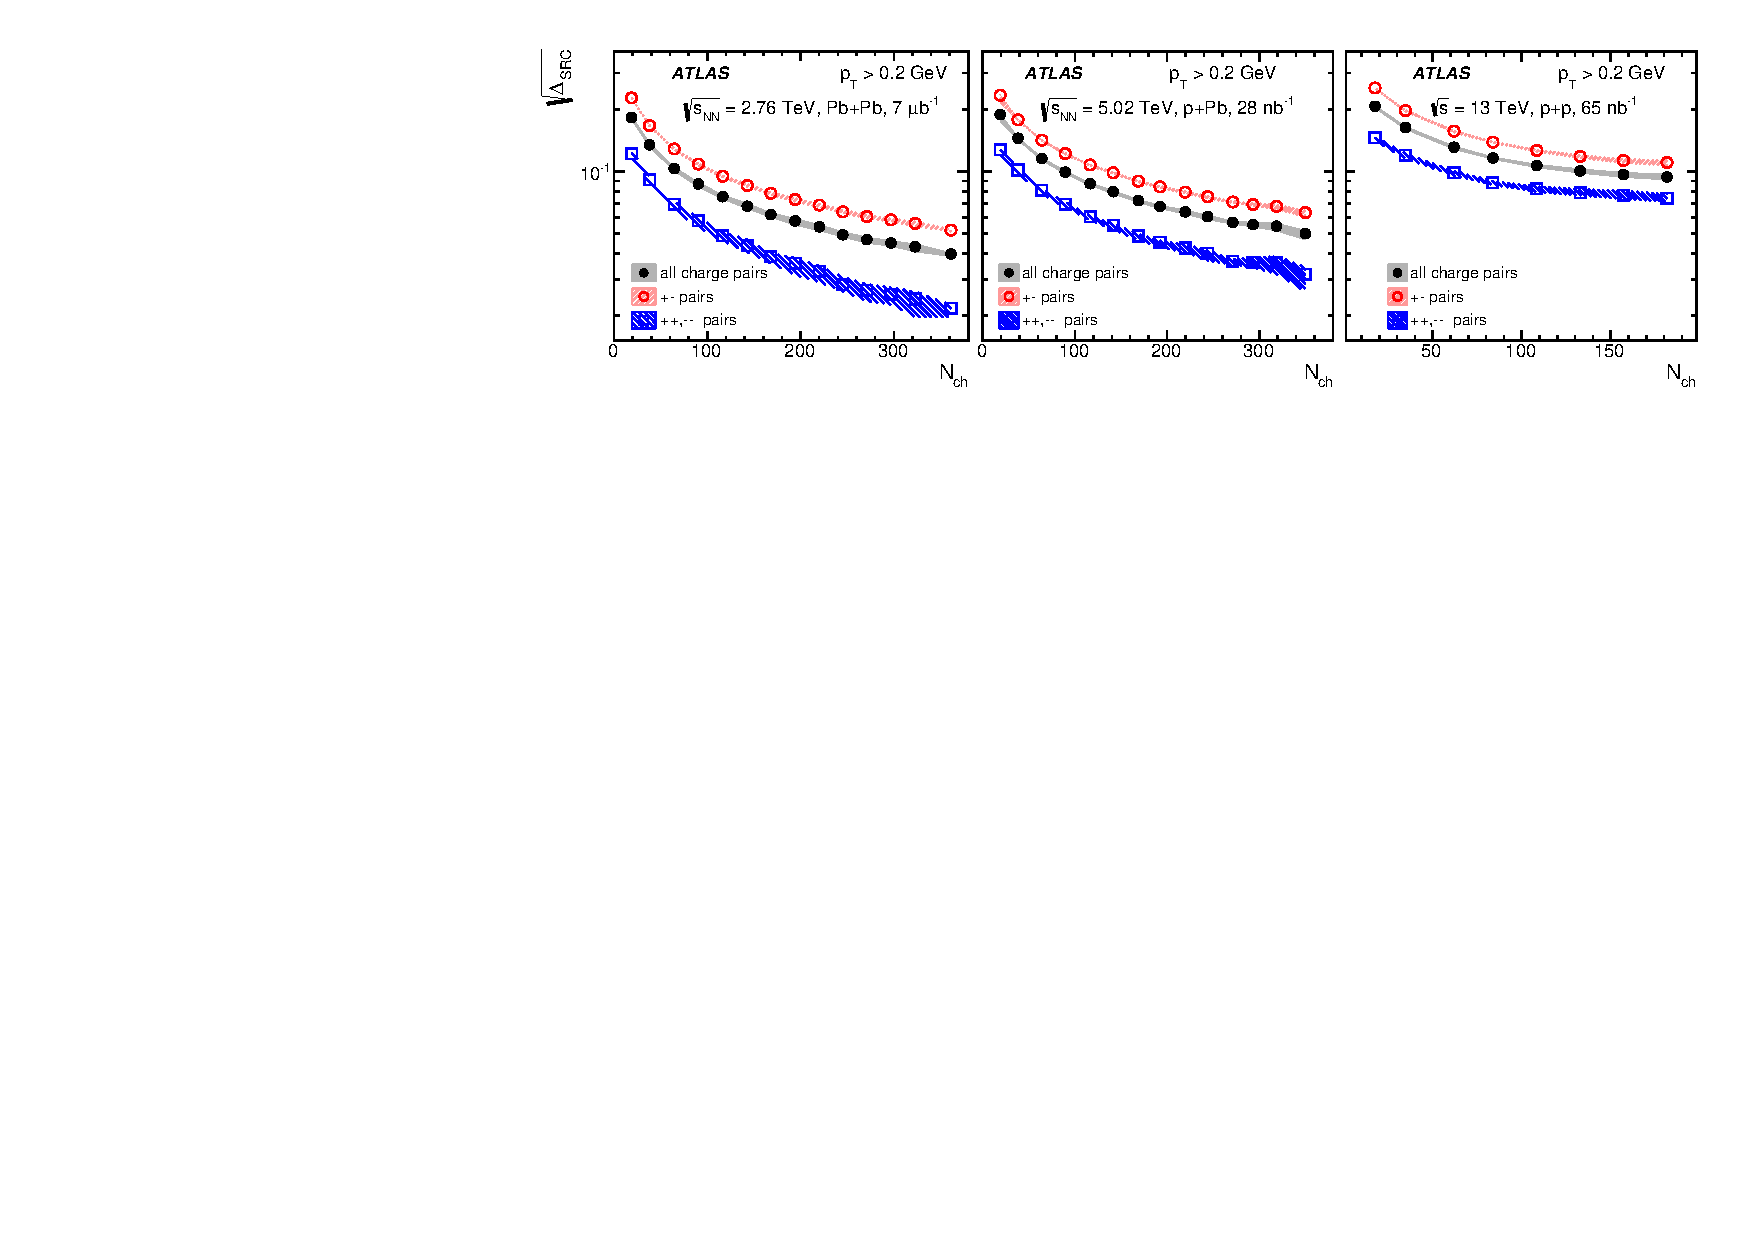
\includegraphics[width=.95\linewidth]{figs/chapter_fbcorr/ATLAS_SRC_charge.pdf}
\caption{The estimated magnitude of the short-range component $\sqrt{\Delta_\text{SRC}}$ as a function of $\Nch$ for all-charge, opposite-charge and same-charge pairs in Pb+Pb (left), $p$+Pb (middle) and $pp$ collisions. The shaded hands represent the systematic uncertainties, and the statistical uncertainties are smaller than the symbols.}
\label{fig:fbcorr_ATLAS_SRC_charge}
\end{figure}

Figure~\ref{fig:fbcorr_ATLAS_SRC_LRC} compares the strength of the SRC in terms of $\sqrt{\Delta_\text{SRC}}$ and the LRC in terms of $\sqrt{\lr{a_1^2}}$ for the three collision systems. The values of $\sqrt{\Delta_\text{SRC}}$ are observed to differ significantly while the values of $\sqrt{\lr{a_1^2}}$ agree within $\pm 10\%$ between the three collision systems.

The strength of SRC and LRC can be related to the number of cluster $n$ contributing to the final multiplicity $\Nch$, where $n$ is the sum of clusters from the projectile and target nucleon or nucleus, $n=n_\text{F} + n_\text{B}$. The LRC is expected to be related to the asymmetry between $n_\text{F}$ and $n_\text{B}$:
\begin{equation}
\begin{split}
A_n &= \frac{n_\text{F} - n_\text{B}}{n_\text{F} + n_\text{B}} \\
\lr{a_1^2} &\propto \lr{A_n^2}
\end{split}
\end{equation}
The clusters could include the participating nucleons, sub-nucleonic degrees of freedom such as the fragmentation of scattered partons, or resonance decays. In an independent cluster model~\cite{Berger:1974vn}, each cluster emits the same number of pairs and the number of clusters follow Poisson fluctuations. In this picture, both the SRC in terms of $\Delta_\text{SRC}$ and LRC in terms of $\lr{a_1^2}$ should scale approximately as the inverse of the number of clusters, and hence, assuming $n$ and $\Nch$ are proportional, the $\sqrt{\Delta_\text{SRC}}$ and $\sqrt{\lr{a_1^2}}$ values in Figure~\ref{fig:fbcorr_ATLAS_SRC_LRC} are expected to follow a simple power-law function in $\Nch$:
\begin{equation}
\sqrt{\Delta_\text{SRC}} \sim \sqrt{\lr{a_1^2}} \sim \frac{1}{n^\alpha} \sim \frac{1}{\Nch^\alpha}, \alpha \approx 0.5.
\end{equation}
A power index that is less than one half, $\alpha<0.5$, would suggest that $n$ grows more slowly than $\Nchrec$, and vice versa.

To test this idea, the $\sqrt{\Delta_\text{SRC}}$ and $\sqrt{\lr{a_1^2}}$ data in Figure~\ref{fig:fbcorr_ATLAS_SRC_LRC} are fitted to a power-law function: $c / \Nch^\alpha$. The function describes the $\Nch$ dependence in all three collision systems, with a reduced $\chi^2$ values ranging between 0.2 and 0.9. The extracted power index values are summarized in Table~\ref{table:fbcorr_ATLAS_power_index}. The values of $\alpha$ for the SRC are found to be smaller for smaller collision systems, they are close to 0.5 in the Pb+Pb collisions and are significantly smaller than 0.5 in the $pp$ collisions. In contrast, the values of $\alpha$ for $\sqrt{\lr{a_1^2}}$ agree within uncertainties between the three systems and are slightly below 0.5.

\begin{figure}[H]
\centering
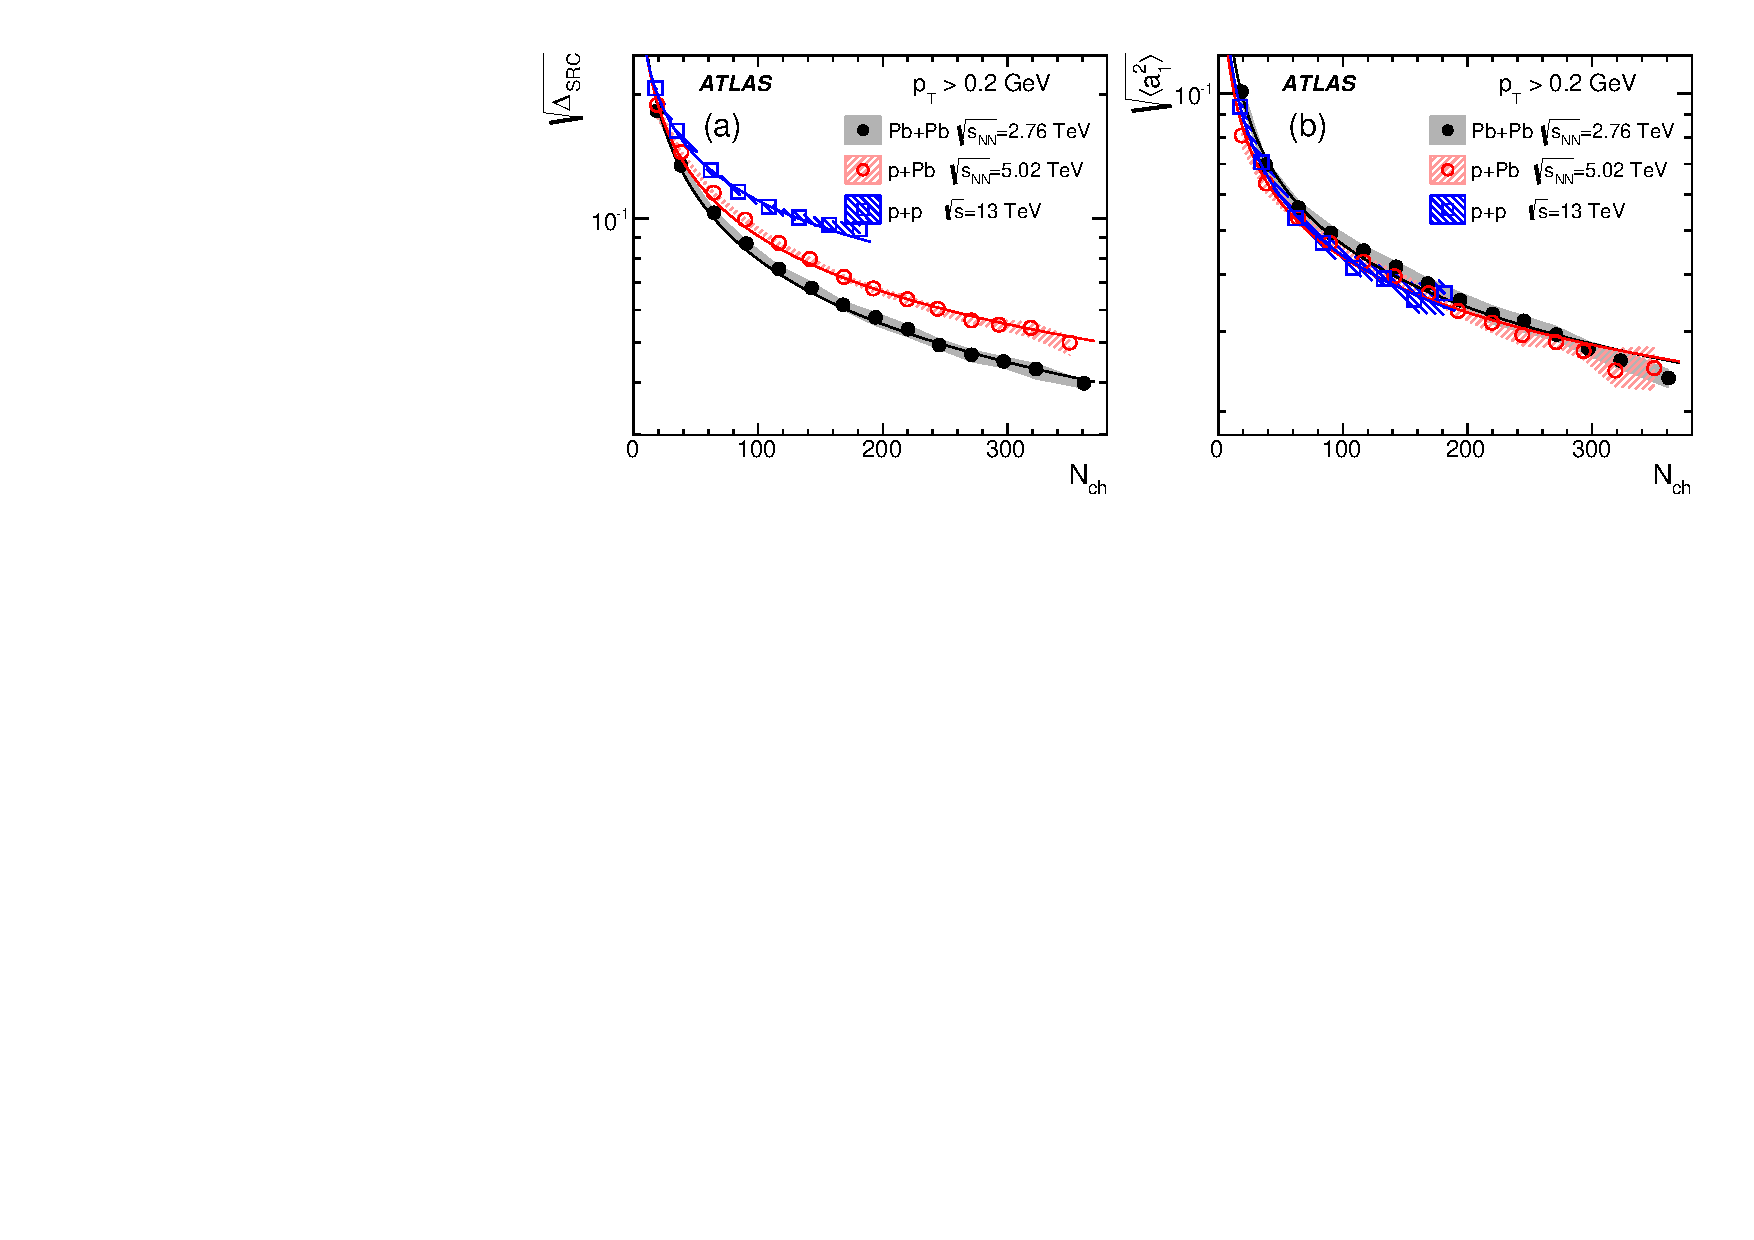
\includegraphics[width=.95\linewidth]{figs/chapter_fbcorr/ATLAS_SRC_LRC.pdf}
\caption{The estimated magnitude of the short-range component $\sqrt{\Delta_\text{SRC}}$  (left) and $\sqrt{\lr{a_1^2}}$ (right) values as a function of $\Nch$ for all-charge pairs in Pb+Pb, $p$+Pb and $pp$ collisions. The shaded bands represent the systematic uncertainties, and the statistical uncertainties are smaller than the symbols.}
\label{fig:fbcorr_ATLAS_SRC_LRC}
\end{figure}

\begin{table}[H]
\centering
\begin{tabular}{|llll|}
\hline
                                        & Pb+Pb                          & $p$+Pb                         & $pp$                           \\ \hline
$\alpha$ for $\sqrt{\Delta_\text{SRC}}$ & 0.505 $\pm$ 0.011 & 0.450 $\pm$ 0.010 & 0.365 $\pm$ 0.014 \\
$\alpha$ for $\sqrt{\lr{a_1^2}}$        & 0.454 $\pm$ 0.011 & 0.433 $\pm$ 0.014 & 0.465 $\pm$ 0.018 \\ \hline
\end{tabular}
\caption{The power index and associated total uncertainty from a power-law fit of the $\Nch$ dependence of $\sqrt{\Delta_\text{SRC}}$ and $\sqrt{\lr{a_1^2}}$.}
\label{table:fbcorr_ATLAS_power_index}
\end{table}

One striking feature of the correlation function in $p$+Pb collisions, for example in Figure~\ref{fig:fbcorr_ATLAS_corr_2D}, is a large FB asymmetry of the SRC, $\delta_\text{SRC}(\eta_1, \eta_2)$ along the $\eta_+$ direction. Even in $pp$ collisions, the $\delta_\text{SRC}$ distribution is not uniform, but instead shows a quadratic increase towards large $|\eta_+|$ values. According to the discussion above, the shape of the $\delta_\text{SRC}$ distribution in $\eta_+$ is described by the $f(\eta_+)$. Examples of the $f(\eta_+)$ are shown in Figure~\ref{fig:fbcorr_ATLAS_SRC_shape} for $p$+Pb, symmetrized $p$+Pb, $pp$ and Pb+Pb collisions with $100 \le \Nchrec < 120$, where symmetrized $p$+Pb results are obtained by averaging the proton-going and lead-going directions such that $C(\eta_1, \eta_2) = C(-\eta_1, -\eta_2)$.

The independent cluster picture discussed above offers a simple interpretation of the shape of $f(\eta_+)$. Assuming the population of clusters is a function of $\eta$, $n_c(\eta)$, and on average each cluster produces $m$ charged particles according to a Poisson distribution, then the number of the SRC pairs scales as $n_c\lr{m(m-1)}=n_c\lr{m}^2$ and the number of the combinatorial pairs scales as $(n_c\lr{m})^2$. Therefore the strength of the SRC at given $\eta$ is expected to scale as
\begin{equation}
\delta_\text{SRC}(\eta, \eta) \propto \frac{n_c \lr{m(m-1)}}{(n_c\lr{m})^2} = \frac{1}{n_c} \propto \frac{1}{d\Nch / d\eta},
\end{equation}
where $n_c(\eta)$ is assumed to be proportional to the local charge-particle multiplicity density $d\Nch / d\eta$. Hence, the fact that $f(\eta_+)$ is larger in the proton-going direction than in the lead-going direction in $p$+Pb collisions simply reflects the asymmetric shape of the $d\Nch / d\eta$ distribution in each event~\cite{ATLAS:2011ag}. The quadratic shape of $f(\eta_+)$ for $pp$ and symmetrized $p$+Pb systems therefore reflects a large, intrinsic FB asymmetry of $d\Nch / d\eta$ on an event-by-event level. The FB asymmetry in $pp$ collisions is lightly larger than $p$+Pb collisions at comparable $\Nch$, but is significantly less in Pb+Pb collisions. This observation suggests that the FB asymmetry for particle production in $pp$ collisions could be as large as that in $p$+Pb collisions at comparable event activity, whereas the FB asymmetry for particle production is smaller in Pb+Pb collisions.

\begin{figure}[H]
\centering
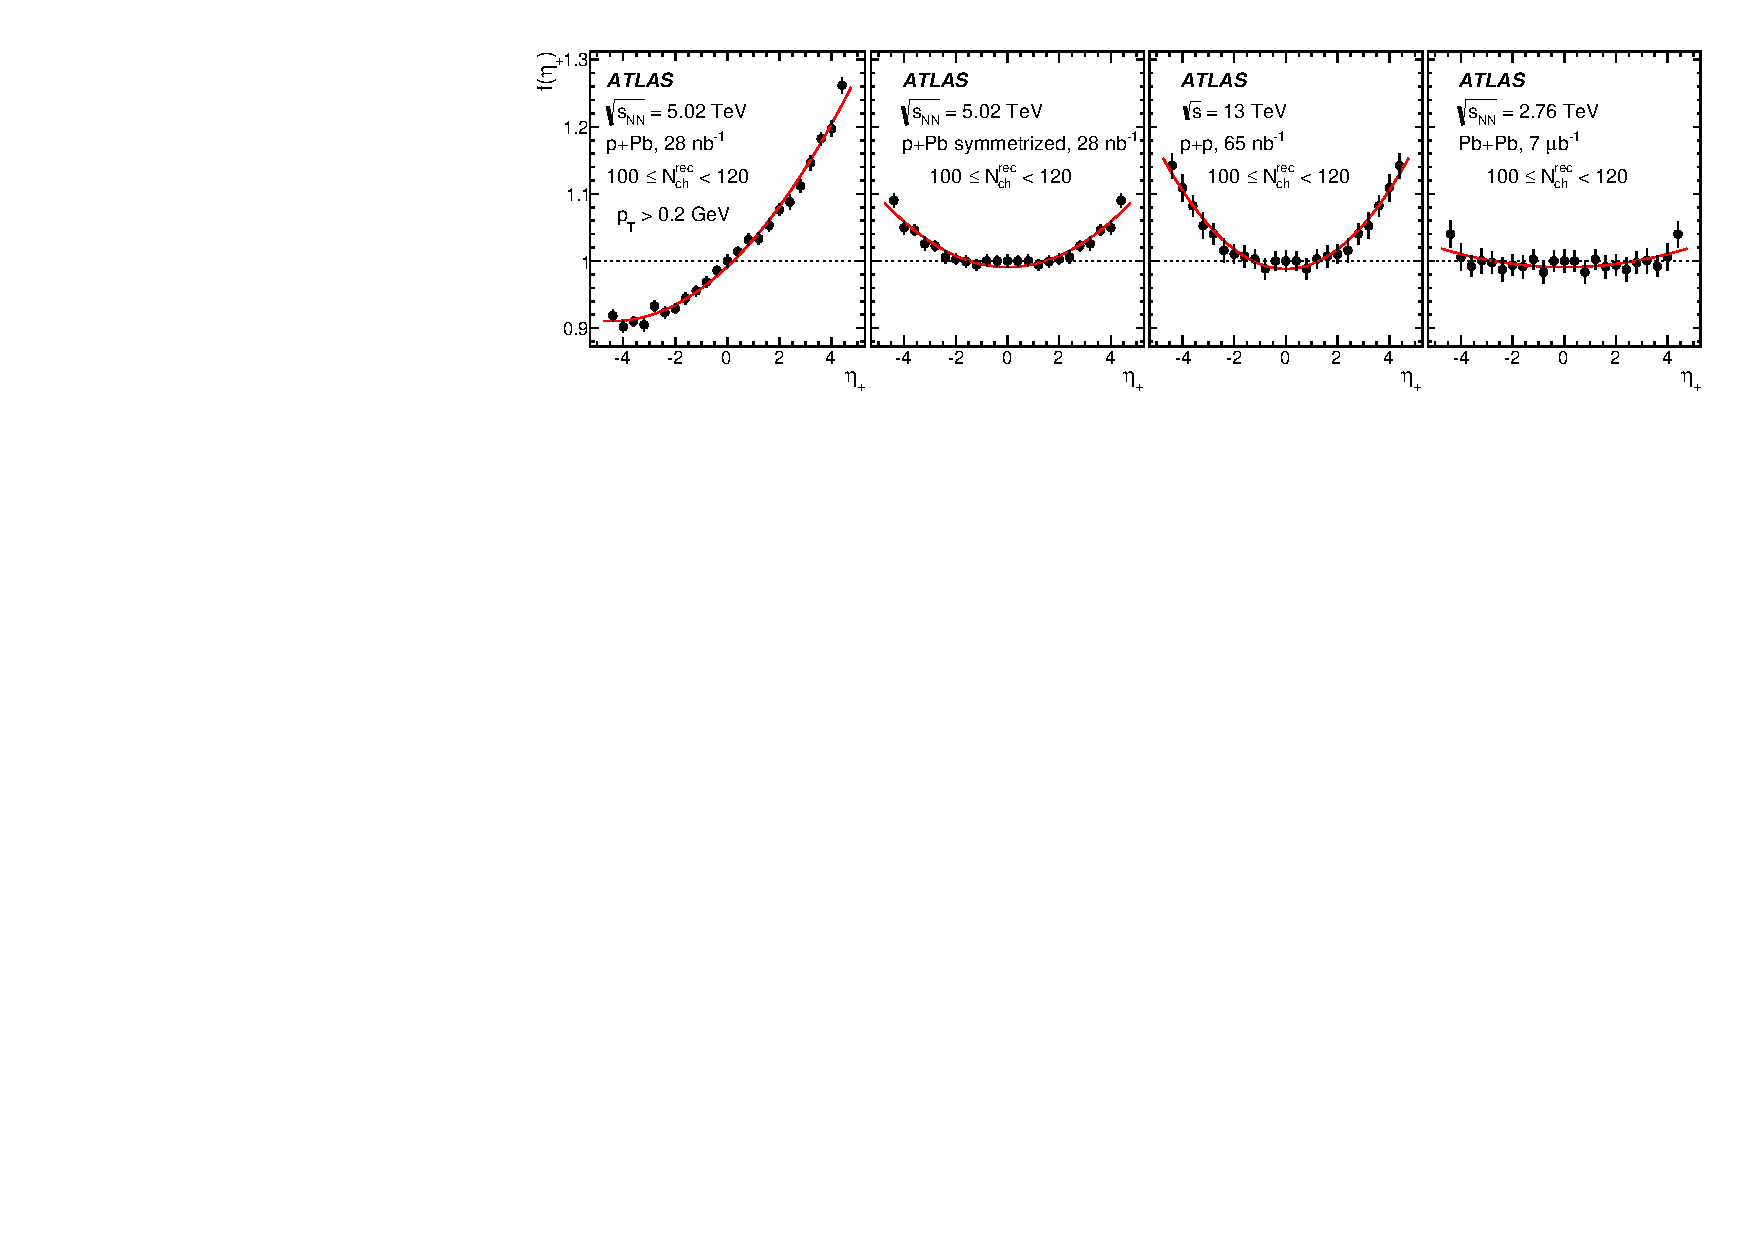
\includegraphics[width=.95\linewidth]{figs/chapter_fbcorr/ATLAS_SRC_shape.pdf}
\caption{The shape of the SRC in $\eta_+$ represented by $f(\eta_+)$ calculated for $p$+Pb, symmetrized $p$+Pb, $pp$ and Pb+Pb collisions with $100 \le \Nchrec < 120$. The solid lines represent a fit to a quadratic function.}
\label{fig:fbcorr_ATLAS_SRC_shape}
\end{figure}

QCD-inspired models such as PYTHIA and EPOS are often used to describe the particle production in $pp$ collisions. ATLAS has previously compared the predictions of the PYTHIA 8 A2 and EPOS LHC tunes with various single-particle distributions, such as the $\pT$, $\eta$ and the event-by-event $\Nch$ distributions, fully unfolded for detector effects~\cite{Aad:2016mok, Aaboud:2016itf}. Reasonable agreement has been observed for these single-particle observables. In order to perform a data model comparison, the multiplicity correlation procedure used on the data is repeated for the two models to extract the SRC and LRC components. The extracted LRC in these models is then decomposed into Legendre coefficients of different order. The coefficients are found to be dominated by $\sqrt{\lr{a_1^2}}$, consistent with the observation that the shapes of the LRC are similar to those in the $pp$ data in Figure~\ref{fig:fbcorr_ATLAS_corr_2D}. However, the values of $\sqrt{\lr{a_1^2}}$ predicted by the models are found to be much smaller than the $pp$ data at the same $\Nch$.

For a more direct comparison, Figure~\ref{fig:fbcorr_ATLAS_SRC_LRC_modelComp} shows the $\Nch$ dependence of SRC and LRC from the data and the two models in $pp$ collisions. The systematic uncertainties on the model predictions are dominated by the uncertainty in separating the SRC and LRC, as discussed earlier. However, at large $\Nch$, they are also limited by the available MC statistics. There is some indication that the values of $\sqrt{\Delta_\text{SRC}}$ from data are larger than the EPOS predictions and smaller than those from PYTHIA 8. Furthermore, the values from PYTHIA 8 increase for $\Nch>120$, a trend not supported by the data. On the other hand, both models underestimate significantly the values of $\sqrt{\lr{a_1^2}}$, suggesting that the FB multiplicity fluctuations in both models are significantly weaker than in the $pp$ data. Therefore, these two models, which were tuned to describe many single-particle observables, fail to describe the longitudinal correlations between the produced charged particles.

\begin{figure}[H]
\centering
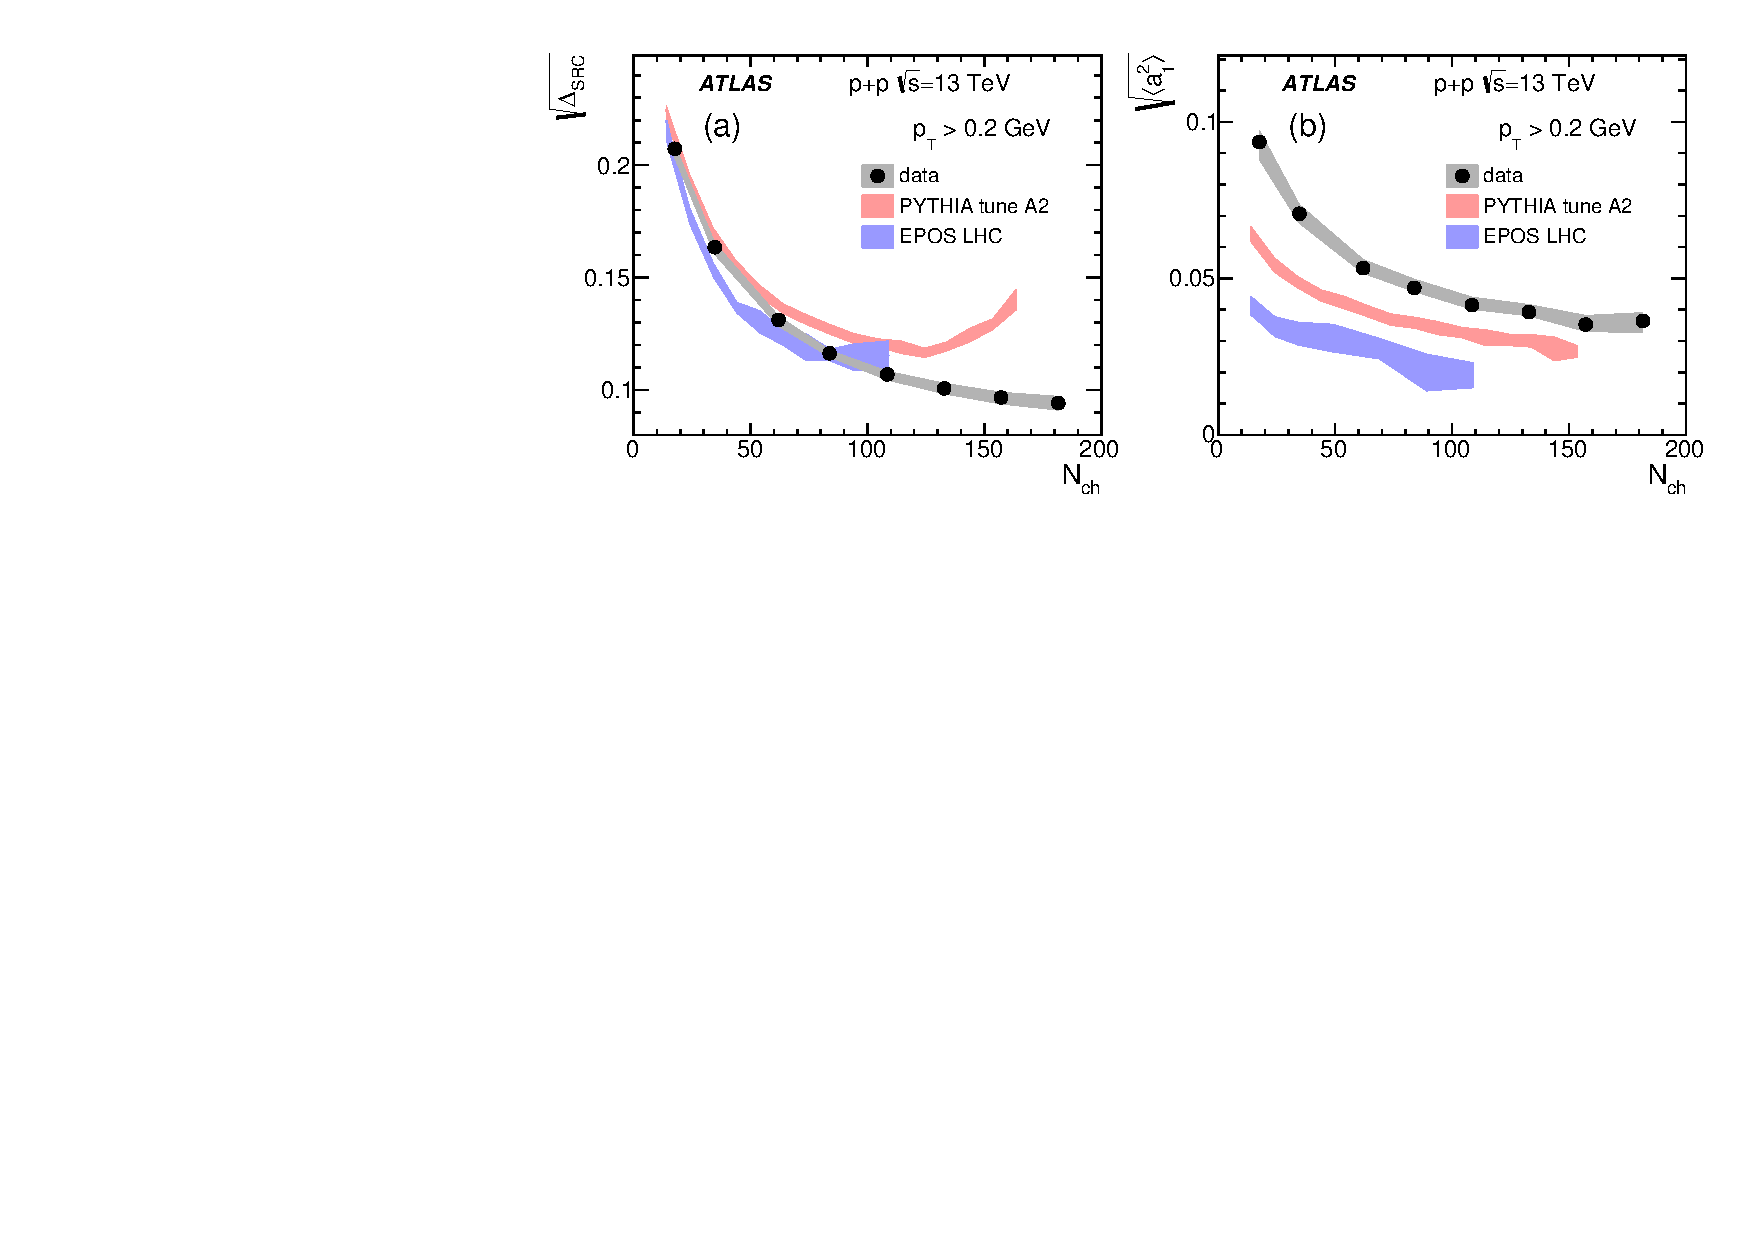
\includegraphics[width=.95\linewidth]{figs/chapter_fbcorr/ATLAS_SRC_LRC_modelComp.pdf}
\caption{The $\sqrt{\Delta_\text{SRC}}$ (left) and $\sqrt{\lr{a_1^2}}$ (right) as a function of $\Nch$ in $pp$ collisions, compared between data and PYTHIA 8 A2 and EPOS LHC. The shaded bands represent the total uncertainties.}
\label{fig:fbcorr_ATLAS_SRC_LRC_modelComp}
\end{figure}



\subsection{Summary and discussion}

In summary, a new method has been proposed to study the longitudinal multiplicity correlations in high-energy nuclear collisions. In this method, events are classified into narrow event activity bins, and EbyE fluctuations are then extracted relative to the average multiplicity distribution in each event activity bin. This procedure allows the separation of the centrality dependence of the multiplicity distribution from the dynamical shape fluctuations. The multiplicity correlations are extracted using the single-particle distribution or two-particle correlation function. The extracted signals are decomposed into a set of orthogonal longitudinal harmonics in terms of Legendre polynomials, which characterize various components of the multiplicity fluctuation of different wavelength in $\eta$.

The first several coefficients $a_n$ are obtained and found to decrease slowly with $n$ in HIJING model but very rapidly with $n$ in AMPT model, which could be due to viscous damping effects of the longitudinal harmonics by the final-state re-scattering effects. The $a_1$ signal is found to strongly correlate with the asymmetry in the number of forward-going and backward-going participating nucleons, which a nonzero $a_2$ signal could be related to the fluctuations of the nuclear stopping or shift of the effective center-of-mass of the collisions. This geometrical origin of the $a_1$ can be experimentally verified by observing an anti-correlation between $a_1$ and the asymmetry of the spectator nucleons detected by the zero-degree calorimeters. Two-particle pseudorapidity correlations also reveal interesting charge-dependent short-range structures in the AMPT model but are absent in the HIJING model, suggesting that these structures are sensitive to the underlying hadronization mechanism. Hence measurement of the multiplicity fluctuation in terms of longitudinal harmonics provides an promising avenue for understanding the particle production mechanism in the early stage of the heavy-ion collisions and for probing the final-state re-scattering effects.

Two-particle pseudorapidity correlations are also measured with the ATLAS detector in Pb+Pb, $p$+Pb and $pp$ collisions. The correlation function $C_\text{N}(\eta_1, \eta_2)$ is measured using charged particles in pseudorapidity range $|\eta|<2.4$ with transverse momentum $\pT>0.2$ GeV, and it is measured as a function of event multiplicity $\Nch$ defined by the total number of charged particles with $|\eta|<2.5$ and $\pT>0.4$ GeV. The correlation function shows an enhancement along the $\eta_1 \approx \eta_2$ direction and suppression at $\eta_1 \approx -\eta_2 \sim \pm 2.4$, consistent with the expectation from an event-by-event forward-backward asymmetry in the multiplicity fluctuation: the long-range correlations or LRC. However, the correlation function also has a large narrow ridge along the $\eta_1 \approx \eta_2$ direction associated with the SRC. The magnitudes of the SRC in $p$+Pb is found to be larger in the proton-going direction than the lead-going direction, reflecting the fact that the particle multiplicity is smaller in the proton-going direction. This is consistent with the observation that the SRC strength increases for smaller $\Nch$. The SRC is observed to be much stronger for opposite-charge pairs than for the same-charge pairs, while the LRC is found to be similar for the two charge combinations. Based on this, a data-driven subtraction method was developed to separate the SRC and LRC. The magnitudes of the SRC and the LRC are then compared for the three collision systems at similar values of $\Nch$.

After subtracting out the $SRC$ $\delta_\text{SRC}(\eta_1, \eta_2)$, the correlation function $C_\text{N}^\text{sub}(\eta_1, \eta_2)$ is decomposed into a sum of products of Legendre polynomials that describe the different shape components, and the coefficients $\lr{a_n a_m}$ are calculated. Significant values are observed for $\lr{a_1^2}$ in all $\Nch$ ranges and higher-order coefficients are consistent with zero, and suggesting that $C_\text{N}^\text{sub}$ has an approximate function form $C_\text{N}^\text{sub} \approx 1 + \lr{a_1^2}\eta_1\eta_2$. The quantity $\lr{a_1^2}$ is also estimated by parameterization of the shape of the correlation function in narrow ranges of $\eta_- = \eta_1 - \eta_2$ and $\eta_+ = \eta_1 + \eta_2$, or from a ratio $C_\text{N}^\text{sub}(\eta_1, \eta_2) / C_\text{N}^\text{sub}(-\eta_1, \eta_2)$, and consistent results are obtained. The magnitude of the SRC and $\sqrt{\lr{a_1^2}}$ are compared for the three collision systems as a function of $\Nch$. Large differences are observed for the SRC, but the values of $\sqrt{\lr{a_1^2}}$ are comparable for the three collision systems as a function of $\Nch$: the values of $\sqrt{\lr{a_1^2}}$ agree within $\pm 10\%$ at the same $\Nch$. The $\Nch$ dependences of both the SRC and $\sqrt{\lr{a_1^2}}$ follow an approximate power-law shape. The power index for $\sqrt{\lr{a_1^2}}$ is approximately the same for the three collision systems. In contrast, the power-law index for the SRC is smaller for smaller collision systems. The SRC distribution shows strong dependence on $\eta_+$ in $p$+Pb and $pp$, but much weaker dependence in Pb+Pb collisions. The $\delta_\text{SRC}(\eta_+)$ distribution, after symmetrizing the proton and lead directions, is found to be similar to the SRC in $pp$ collisions with comparable $\Nch$, suggesting that the EbyE FB asymmetry for particle production is similar in $pp$ and $p$+Pb collisions with comparable event activity. The PYTHIA 8 A2 and EPOS LHC models, which were tuned to describe many single-particle observables in $pp$ collisions, fail to describe the SRC and the LRC observed in the $pp$ data.

Since our method correlates event activities between separate rapidity ranges, it provides a useful way to unfold and quantify the centrality correlations between different rapidity ranges.




\subsection{Outlook}

\subsubsection{Generalization of the observable}

The correlation method discussed in this paper can be generalized into correlation between multiplicity of particles of any two different types. For example, one can measure the correlation between multiplicity for positive and negative particles:
\begin{equation}
C^{+-}(\eta_1, \eta_2) = \frac{\lr{N^+(\eta_1)N^-(\eta_2)}}{\lr{N^+(\eta_1)}\lr{N^-(\eta_2)}},
\end{equation}
which allow the extraction of $\lr{a_n^+ a_n^-}$. Assuming equal multiplicity for positive and negative particles, the coefficients for positive particle $a^+_n$ and negative $a^-_n$ are related to those for inclusive particles via:
\begin{equation}
\lr{a_n^2} = \frac{1}{4}(\lr{a_n^+ a_n^+} + \lr{a_n^- a_n^-} + 2\lr{a_n^+ a_n^-}).
\end{equation}
Due to local charge conservation effects, the correlation between positive and negative particles is expected to be stronger than inclusive correlation. Indeed the AMPT or HIJING simulation studies suggest that
\begin{equation}
\lr{a_n^+ a_n^-} > \lr{a_n^2} > \lr{a_n^+ a_n^+} = \lr{a_n^- a_n^-}.
\end{equation}
The results shown in Figure.~\ref{fig:fbcorr_Model_corr_chargeComp} implies that the dip around $\eta_1 \sim \eta_2$ seen in the inclusive correlation for AMPT model arises mainly from same-charge pairs, although the opposite-charge pair correlation also shows a shallow dip. Such dip is absent in HIJING events independent of the charge combination. These structures reflect the important role of the final-state interaction and hadronization mechanism (via simple coalescence in AMPT) on the charge-dependent correlations.

\begin{figure}[H]
\centering
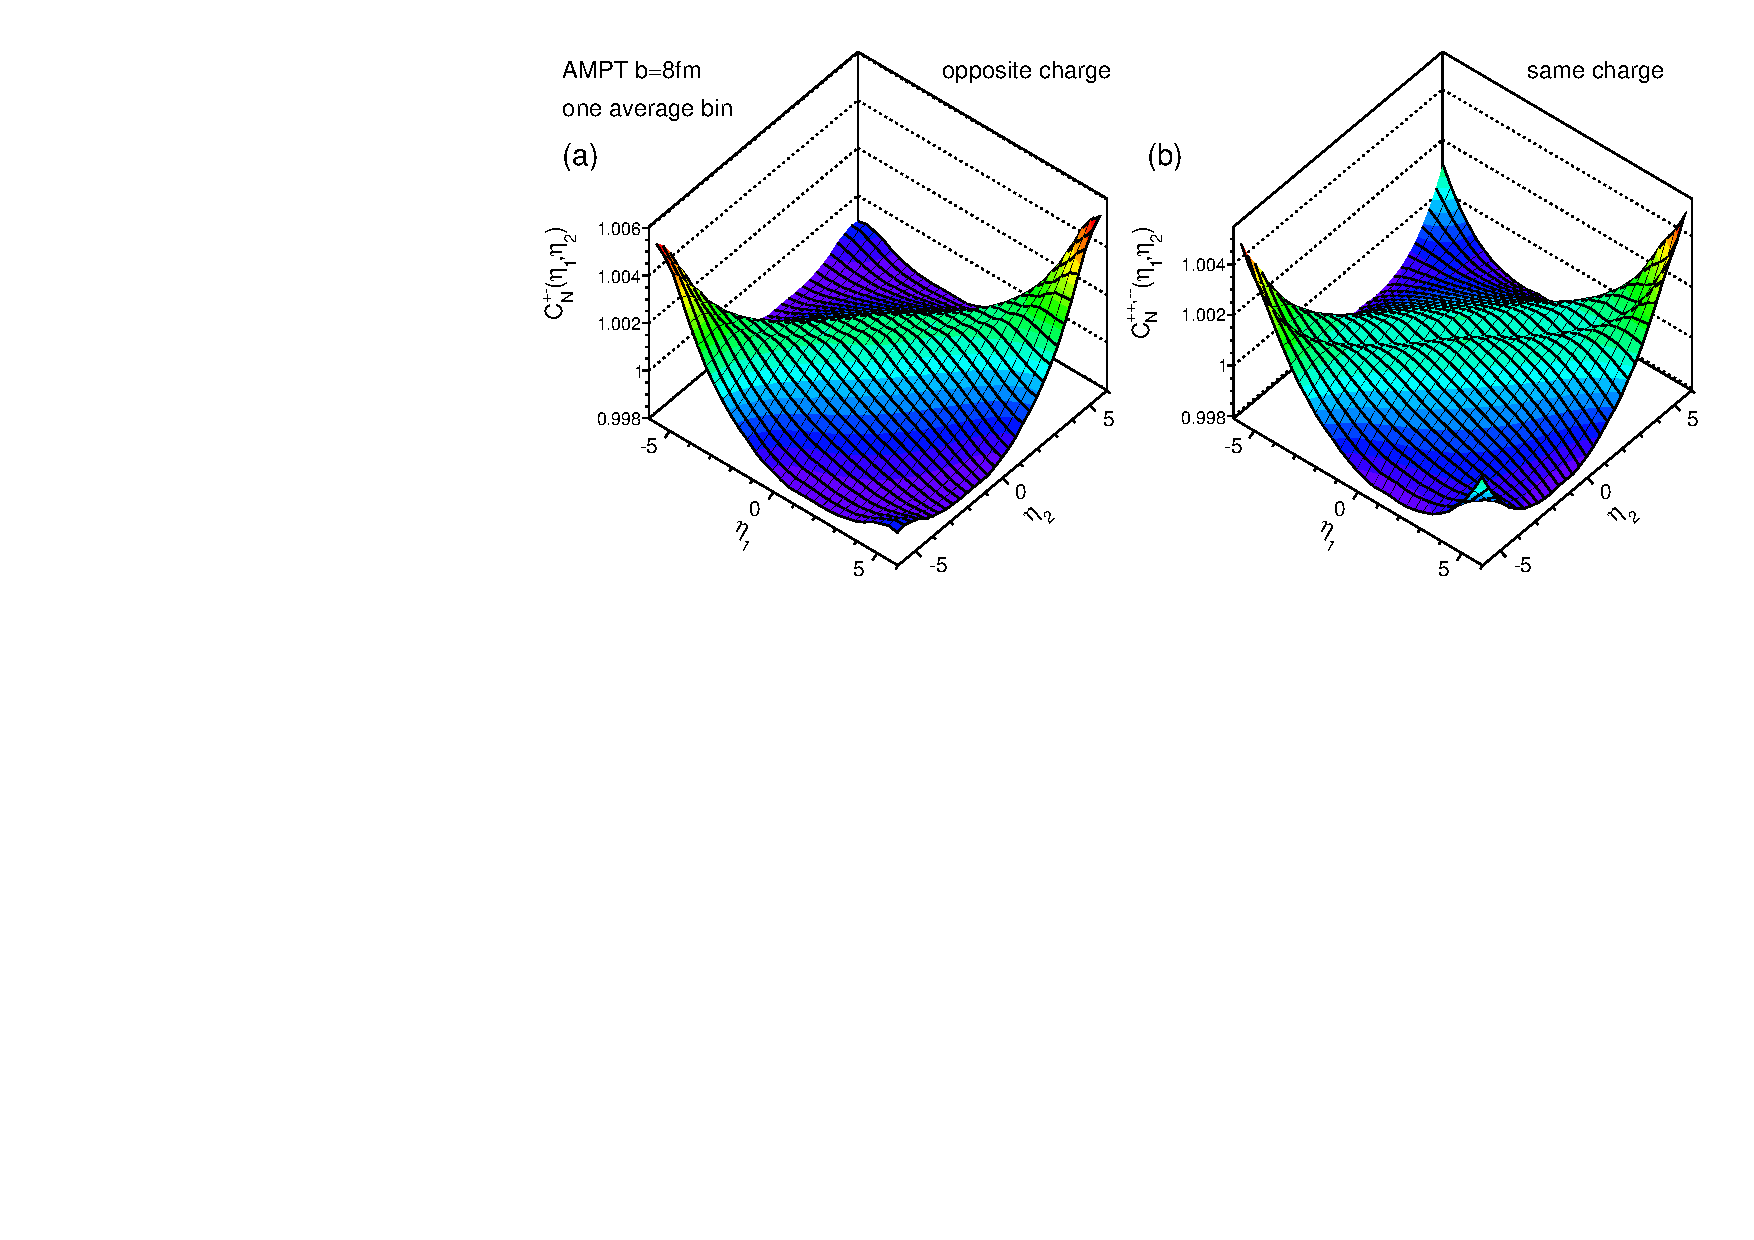
\includegraphics[width=.95\linewidth]{figs/chapter_fbcorr/Model_corr_chargeComp.pdf}
\caption{The correlation functions for same-charge pairs (left) and opposite-charge pairs (right) for AMPT events generated with $b=8$ fm.}
\label{fig:fbcorr_Model_corr_chargeComp}
\end{figure}

Note that the charge-dependent correlation function is related to the well-known balance function $B(\Delta\eta)$~\cite{Bass:2000az}:
\begin{equation}
2 B(\Delta\eta) = 2 C^{+-}(\Delta\eta) - C^{++}(\Delta\eta) - C^{--}(\Delta\eta).
\end{equation}
The stronger correlation strength for opposite-charge pairs than the same-charge pairs as shown in Figure~\ref{fig:fbcorr_Model_corr_chargeComp} implies that the balance function should peak around $\Delta\eta = \eta_1 - \eta_2 = 0$ and fall slowly to large $\Delta\eta$ (i.e., not sensitive to the dips), consistent with earlier observations~\cite{Adams:2003kg, Abelev:2013csa}.

Similarly, one could also divide particles into high $\pT$ and low $\pT$ with equal multiplicity. In this case, the coefficients can be written as
\begin{equation}
\lr{a_n^2} = \frac{1}{4}(\lr{a_n^H a_n^H} + \lr{a_n^L a_n^L} + 2 \lr{a_n^H a_n^L}),
\end{equation}
where $a_n^H$ and $a_n^L$ are coefficients for high-$\pT$ and low-$\pT$ particle multiplicity, respectively. We observe that $\lr{a_n^H a_n^H} > \lr{a_n^H a_n^L} > \lr{a_n^L a_n^L}$ (not shown), presumably due to short-range correlations related to jet fragmentation, which are stronger for higher $\pT$ particles.

It would be also interesting to study the factorization behavior of the multiplicity correlation by calculating a factorization ratio, similar to what is often used in azimuthal flow correlation analysis~\cite{Gardim:2012im}:
\begin{equation}
r_n = \frac{a_n^H a_n^L}{\sqrt{a_n^H a_n^H} \sqrt{a_n^L a_n^L}}.
\end{equation}
The breaking of the factorization can be used to understand the $\pT$ dependence of the long-range and short-range correlations.



\subsubsection{Projections in Run 3 and Run 4}

As shown with ATLAS data (Section~\ref{sec:fb_atlas_data}), significant values are observed for $a_1$ in all multiplicity ranges of $p$+Pb collisions and higher-order coefficients are consistent with zero, which implies the FB multiplicity correlation is dominated by the linear component of the Legendre polynomials. However, several theoretical studies suggest a non-linear component should exist in the region $|\eta|>2.5$~\cite{Bzdak:2012tp, Bhalerao:2014mua}. The increased tracking acceptance and increase in luminosity in Run 4 will provide a great opportunity to measure possible deviation beyond the linear component of the Legendre polynomials.

The top panel of Figure~\ref{fig:fbcorr_ATLAS_a1_run4} shows the projection of $C(\eta_1, \eta_2)$ distributions for same-charge pairs into one-dimensional $\eta_-(\equiv \eta_1 - \eta_2)$ distributions over a narrow slice $|\eta_1 + \eta_2|<0.4$. The distributions are denoted by $C^{\pm\pm}(\eta_-)$. The red quadratic curve represent the linear component and the relative difference between $C^{\pm\pm}(\eta_-)$ and linear component is shown in the bottom panel panel. Short-range correlation contributes to the peak in the range $|\eta_-|<1.0$, while in the long-range region, $|\eta_-|>1.0$, $C^{\pm\pm}(\eta_-)$ is consistent with the linear component. To estimate the Run 4 projection, the magnitude of the first non-linear component, $a_2$, is assumed to be $15\%$ of  the magnitude of $a_1$. The statistical precision is sufficient to quantitatively distinguish the possible non-linear component from the linear component. This projection suggests the Run 4 should bring a better understanding of the early-time density fluctuations in pseudorapidity.

\begin{figure}[H]
\centering
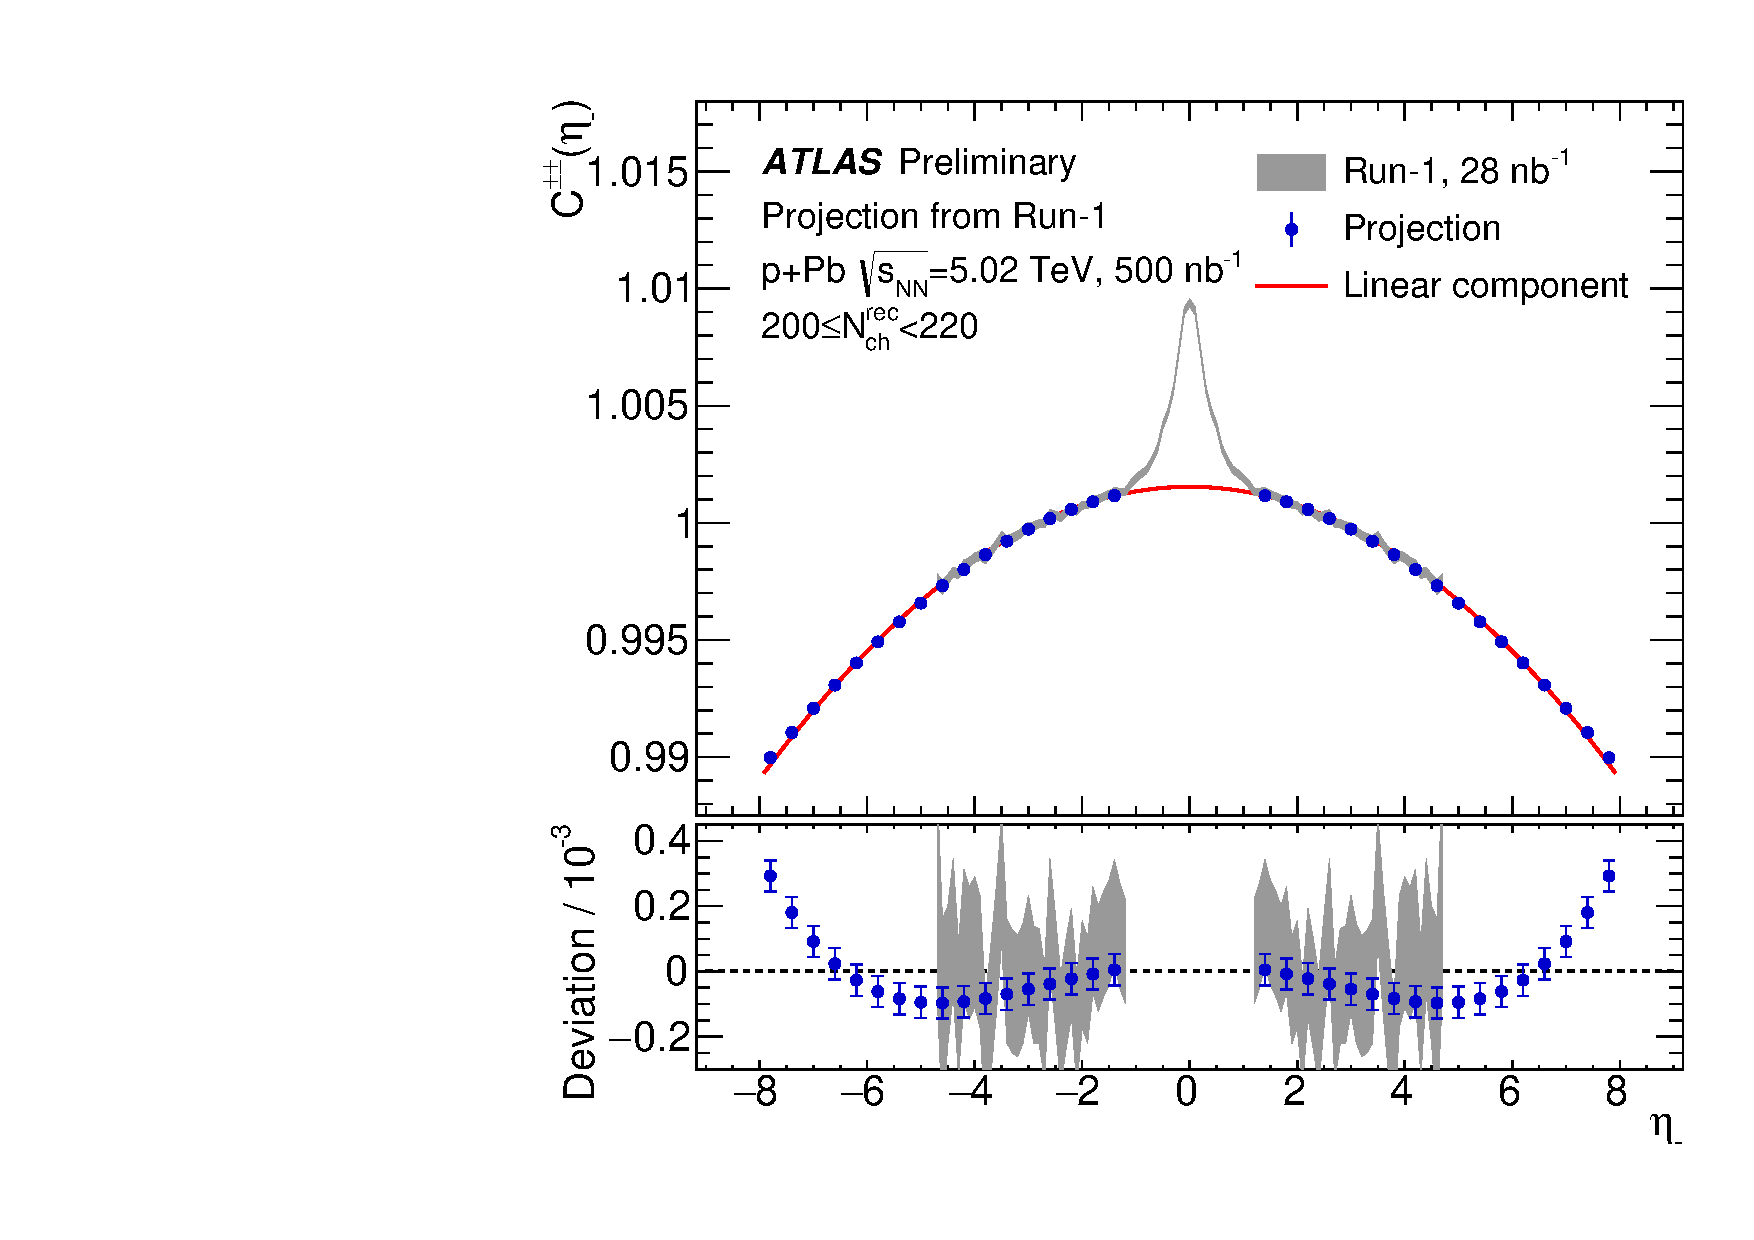
\includegraphics[width=.7\linewidth]{figs/chapter_fbcorr/ATLAS_a1_run4.pdf}
\caption{Projection of $C(\eta_1, \eta_2)$ distributions for same-charge pairs ($\pm\pm$) into one-dimensional $\eta_-(\equiv \eta_1 - \eta_2)$ distributions over a narrow slice $|\eta_1 + \eta_2| < 0.4$. In the top panel, the grey band represents the measurement using Run 1 $p$+Pb data and the red curve represents the linear component. The projected Run 4 results are indicated by the blue circles. The relative difference between $C^{\pm\pm}(\eta_-)$ and linear component is shown in the bottom panel.}
\label{fig:fbcorr_ATLAS_a1_run4}
\end{figure}


